% Seção sobre testes de desempenho

\chapter{Testes de desempenho}
%POR QUÊ

Com o objetivo de avaliar o desempenho do algoritmo desenvolvido, foram realizados testes
que permitiram comparar o desempenho das diferentes abordagens.
Foi medido o tempo tomado pelos algoritmos
ao se encontrar repetidamente o ACMP entre os nós folhas de uma árvore.
Com esses dados, analisados

Um programa foi desenvolvido, também na linguagem C++, para realizar os testes de desempenho.
Foi utilizada a funcionalidade de templates da linguagem para facilitar a definição equivalente dos testes para todos os algoritmos, mas ainda assim permitir que o compilador otimizasse as chamadas, evitando custos adicionais durante os testes devido à hierarquia de classes utilizada.
O programa depende da biblioteca do hwloc.
Os valores medidos são escritos em um arquivo no formato CSV (Valores Separados por Vírgula -- \textit{Comma-Separated Values})


\section{Máquinas utilizadas nos testes}

Os testes foram executados sobre duas máquinas (\textit{notebooks}), que serão identificadas como Máquina~A e Máquina~B, para as quais o programa lstopo gera as representações de hierarquia apresentadas na Figura \ref{img:maquinas}.
Estas representações revelam o tamanho das memórias cache, que podem ter efeito nos resultados dos testes.
A Tabela \ref{tab:maquinas} apresenta mais detalhes de ambas.

% Tabela comparando as máquinas
\begin{table}[htb]
	\newcommand \mesmo[1] {\multicolumn{2}{c}{#1}}
	\centering
	\caption{Características das máquinas utilizadas nos testes}%
	\label{tab:maquinas}
	%{
	\begin{tabular}{ccc}
		\toprule
		& Máquina A & Máquina B\\
		\midrule
		Sistema Operacional
			%& ---
			& \mesmo{\begin{tabular}{@{}c@{}}
				Windows 10 Home\\64 \textit{bits}\end{tabular}} \\
			%(10.0, Compilação 14393)
			%(10.0, Compilação 15063) \\
			%& ---
			%& 64 \textit{bits} \\
		\midrule
		\multirow{3}{*}{Processador}
			%& ---
			& \mesmo{Intel\textregistered\ Core\texttrademark} \\%, ~2.6GHz \\
			& i5 5200U
			& i7 6600U \\% CPU
			& 2.20 GHz
			& 2.50 GHz \\
			% Cores
			%& ---
			%& 2 \textit{cores}, 4 \textit{threads} \\
		\midrule
		\multirow{3}{*}{Memória Principal}
			% Tipo
			& DDR3
			& DDR4 \\
			% Tamanho
			& 6 GB
			& 8 GB \\
			% Frequência
			& 798.7 MHz
			& 1067 MHz \\
			%
			%& ---
			%&  \\
		\bottomrule
	\end{tabular}
\end{table}

\begin{figure}
	\centering
	\caption{Saída do programa lstopo sobre as máquinas utilizadas}
	\label{img:maquinas}
	\begin{subfigure}{.4\textwidth}
		\caption{Máquina A}
		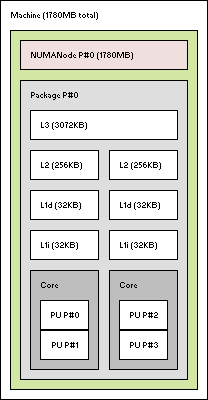
\includegraphics[width=\textwidth]{rec/img/MaqA}
	\end{subfigure}
	~
	\begin{subfigure}{.4\textwidth}
		\caption{Máquina B}
		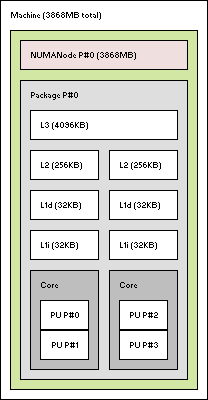
\includegraphics[width=\textwidth]{rec/img/MaqB}
	\end{subfigure}

\end{figure}


\section{Configurações}

Em ambas as máquinas, os testes foram compilados usando a versão 5.3.0 do compilador GCC (\textit{GNU Compiler Collection}) \cite{gcc}, inclusa no projeto Cygwin \cite{cygwin}, o qual emula um sistema Unix em versões atuais do sistema operacional Windows.
Esta versão do GCC era a única disponível no Cygwin durante o desenvolvimento do trabalho com a qual não foram encontrados problemas com funcionalidades da linguagem C++.
Foram usadas as seguintes \textit{flags} de compilação:
\begin{itemize}
	\item \texttt{-std=c++11}: Utiliza funcionalidades do padrão C++11 da linguagem C++
	\item \texttt{-O3}: Ativa diversas otimizações
	\item \textit{flags} obtidas com os comandos \texttt{pkg-config --cflags hwloc} e \texttt{pkg-config --libs hwloc} no Cygwin, que imprimem as \textit{flags} necessárias para utilizar o hwloc
\end{itemize}
%\input{rec/tab/flags}


%COMO
\section{Estrutura dos testes}

Os testes consistem em encontrar repetidamente o ACMP entre os nós folhas de uma dada árvore com os diferentes algoritmos.
Cada vez que as estruturas necessárias são criadas e os testes são executados sobre elas com um determinado algoritmo, obtém-se uma observação, que é o tempo que levou para realizar a quantidade especificada de repetições da função \fACMP\ entre os nós folhas da árvore com o algoritmo.
É usada uma grande quantidade de repetições pois não é possível medir corretamente o tempo de apenas uma chamada à função, o qual é menor que a resolução das chamadas de temporização no processador.

Para cada algoritmo, uma árvore de estrutura equivalente é criada (as estruturas de dados dependem do algoritmo) a partir dos graus fornecidos como entrada.
%(Como os graus são usados para montar a árvore -- se não for explicado antes)
Os graus são recebidos como uma lista de inteiros positivos.
O $i$-ésimo será o grau do nível $i-1$.
Deste modo, se os graus recebidos são $(g_1, g_2, ..., g_n)$, a raiz terá $g_1$ filhos, cada um com $g_2$ filhos, e assim por diante, até os nós do nível $n-1$, que terão $g_n$ filhos cada.

Para obter uma observação de um algoritmo, uma lista contendo todos os pares possíveis de nós folhas (todas as combinações de duas folhas) é criada.
Esta lista é embaralhada, usando uma semente fixa, de modo que a ordem pseudo-aleatória é a mesma para todas as execuções de todos os algoritmos sobre esta árvore.
Isto é feito para evitar que o desempenho dos algoritmos seja beneficiado pelo acesso repetido dos mesmos nós, o que não corresponde a situações reais.

Uma observação é obtida por meio de uma etapa de aquecimento seguida de uma de medição, na qual o tempo total das repetições da função ACMP é medido.
Ambas as etapas consistem em algum número de rodadas, o qual geralmente deve estar na casa de alguns milhares, dependendo do tamanho da árvore, para que o tempo medido seja significativo.
Em cada rodada, a lista previamente embaralhada de pares de folhas é varrida e, para cada par, o ACMP é encontrado usando o algoritmo em questão.

As observações dos diferentes algoritmos são realizadas de forma intercalada.
O número de observações obtidas para cada algoritmo em uma execução do programa depende de dois parâmetros, número de iterações externas e de iterações internas.
O número de iterações internas é a quantidade de observações que serão obtidas para um dos algoritmos antes de passar para outro.
A execução da quantidade de iterações internas para cada algorimo compõe uma iteração externa.
Esta forma de especificar a quantidade de observações originou-se nas etapas iniciais dos testes, para facilitar a visualização dos resultados, mas foi mantida.
No entanto, julga-se melhor usar poucas iterações internas e mais externas para evitar que eventuais condições temporárias da máquina, causadas por elementos externos ao programa, afetem diversas observações de apenas um dos algoritmos.

O programa também permite escolher quais algoritmos serão testados dentre os quatro analisados.

%(Tabela com os parâmetros?)


\subsection{RESULTADOS}

As árvores utilizadas nos testes correspondem à hierarquia de memória de máquinas reais, apresentadas no site do projeto hwloc, como representadas pelo programa lstopo \cite{lstopo}.
Assim, os resultados refletem a diferença dos algoritmos quando operando sobre hierarquias reais.
%\tratar{(Referência: The Best of lstopo - https://www.open-mpi.org/projects/hwloc/lstopo/)}

\tratar{especificar parâmetros utilizados}
Foram usadas, em todas as execuções, mil rodadas na etapa de aquecimento e dez mil, na etapa de medição.

Notou-se a presença de diversos \textit{outliers} de valor significativamente mais baixo nas observações obtidas.
Acredita-se que isso se deva a momentos em que os processos do sistema operacional em segundo plano em conjunto tenham coincidentemente requerido pouco processamento.

Inicialmente, os testes foram feitos sem acessar o ACMP obtido a cada execução, ou seja, para cada par de folhas, simplesmente se encontrava o ponteiro para o ancestral, mas nenhum dado do ancestral era obtido.
No entanto, em cenários reais, os nós seriam buscados para se obter alguma informação sobre eles, portanto, foi adicionado um acesso a um valor qualquer de cada ACMP encontrado para simular isso.
A~Figura~\ref{fig:box_sem_com} compara o desempenho dos quatro algoritmos na Máquina~A para a árvore com os graus $(1, 4, 1, 1, 9, 2, 1, 1, 4)$ antes e depois do acréscimo desse acesso.
%Neste \textit{boxplo}
Sem o acesso foram feitas 300 observações de cada algoritmo e, com o acesso, 150 observações.
Como era esperado, os tempos aumentaram para todos os algoritmos, porém o algoritmo menos afetado foi o novo e o mais afetado foi o da matriz, considerando a porcentagem de aumento do valor mediano após acrescentar o acesso, conforme a Tabela \ref{tab:aumento_mediana}.

\begin{figure}[h]
	\caption{Tempos com e sem acesso ao ACMP}
	\label{fig:box_sem_com}
	\resizebox{\textwidth}{!}{% Title: glps_renderer figure
% Creator: GL2PS 1.3.8, (C) 1999-2012 C. Geuzaine
% For: Octave
% CreationDate: Tue May 30 02:05:50 2017
\begin{pgfpicture}
\pgfsetlinewidth{0.01pt}
\color[rgb]{1.000000,1.000000,1.000000}
\pgfpathmoveto{\pgfpoint{74.882813pt}{47.523438pt}}
\pgflineto{\pgfpoint{74.882813pt}{399.597656pt}}
\pgflineto{\pgfpoint{521.277344pt}{399.597656pt}}
\pgfpathclose
\pgfusepath{fill,stroke}
\pgfpathmoveto{\pgfpoint{521.277344pt}{399.597656pt}}
\pgflineto{\pgfpoint{521.277344pt}{47.523438pt}}
\pgflineto{\pgfpoint{74.882813pt}{47.523438pt}}
\pgfpathclose
\pgfusepath{fill,stroke}
\color[rgb]{0.000000,0.000000,0.000000}
\pgfsetlinewidth{0.500000pt}
\pgfsetdash{{16pt}{0pt}}{0pt}
\pgfpathmoveto{\pgfpoint{521.277344pt}{47.523438pt}}
\pgflineto{\pgfpoint{74.882813pt}{47.523438pt}}
\pgfusepath{stroke}
\pgfpathmoveto{\pgfpoint{521.277344pt}{399.597656pt}}
\pgflineto{\pgfpoint{74.882813pt}{399.597656pt}}
\pgfusepath{stroke}
\pgfpathmoveto{\pgfpoint{74.882813pt}{399.597656pt}}
\pgflineto{\pgfpoint{74.882813pt}{47.523438pt}}
\pgfusepath{stroke}
\pgfpathmoveto{\pgfpoint{521.277344pt}{399.597656pt}}
\pgflineto{\pgfpoint{521.277344pt}{47.523438pt}}
\pgfusepath{stroke}
\pgfpathmoveto{\pgfpoint{102.781250pt}{51.988281pt}}
\pgflineto{\pgfpoint{102.781250pt}{47.523438pt}}
\pgfusepath{stroke}
\pgfpathmoveto{\pgfpoint{102.781250pt}{395.132813pt}}
\pgflineto{\pgfpoint{102.781250pt}{399.597656pt}}
\pgfusepath{stroke}
\pgfpathmoveto{\pgfpoint{158.582031pt}{51.988281pt}}
\pgflineto{\pgfpoint{158.582031pt}{47.523438pt}}
\pgfusepath{stroke}
\pgfpathmoveto{\pgfpoint{158.582031pt}{395.132813pt}}
\pgflineto{\pgfpoint{158.582031pt}{399.597656pt}}
\pgfusepath{stroke}
\pgfpathmoveto{\pgfpoint{214.382813pt}{51.988281pt}}
\pgflineto{\pgfpoint{214.382813pt}{47.523438pt}}
\pgfusepath{stroke}
\pgfpathmoveto{\pgfpoint{214.382813pt}{395.132813pt}}
\pgflineto{\pgfpoint{214.382813pt}{399.597656pt}}
\pgfusepath{stroke}
\pgfpathmoveto{\pgfpoint{270.179688pt}{51.988281pt}}
\pgflineto{\pgfpoint{270.179688pt}{47.523438pt}}
\pgfusepath{stroke}
\pgfpathmoveto{\pgfpoint{270.179688pt}{395.132813pt}}
\pgflineto{\pgfpoint{270.179688pt}{399.597656pt}}
\pgfusepath{stroke}
\pgfpathmoveto{\pgfpoint{325.980469pt}{51.988281pt}}
\pgflineto{\pgfpoint{325.980469pt}{47.523438pt}}
\pgfusepath{stroke}
\pgfpathmoveto{\pgfpoint{325.980469pt}{395.132813pt}}
\pgflineto{\pgfpoint{325.980469pt}{399.597656pt}}
\pgfusepath{stroke}
\pgfpathmoveto{\pgfpoint{381.777344pt}{51.988281pt}}
\pgflineto{\pgfpoint{381.777344pt}{47.523438pt}}
\pgfusepath{stroke}
\pgfpathmoveto{\pgfpoint{381.777344pt}{395.132813pt}}
\pgflineto{\pgfpoint{381.777344pt}{399.597656pt}}
\pgfusepath{stroke}
\pgfpathmoveto{\pgfpoint{437.578125pt}{51.988281pt}}
\pgflineto{\pgfpoint{437.578125pt}{47.523438pt}}
\pgfusepath{stroke}
\pgfpathmoveto{\pgfpoint{437.578125pt}{395.132813pt}}
\pgflineto{\pgfpoint{437.578125pt}{399.597656pt}}
\pgfusepath{stroke}
\pgfpathmoveto{\pgfpoint{493.378906pt}{51.988281pt}}
\pgflineto{\pgfpoint{493.378906pt}{47.523438pt}}
\pgfusepath{stroke}
\pgfpathmoveto{\pgfpoint{493.378906pt}{395.132813pt}}
\pgflineto{\pgfpoint{493.378906pt}{399.597656pt}}
\pgfusepath{stroke}
\color[rgb]{1.000000,0.000000,0.000000}
\pgfsetdash{}{0pt}
\pgfpathmoveto{\pgfpoint{459.898438pt}{92.609375pt}}
\pgflineto{\pgfpoint{415.257813pt}{92.609375pt}}
\pgfusepath{stroke}
\pgfpathmoveto{\pgfpoint{392.937500pt}{320.968750pt}}
\pgflineto{\pgfpoint{370.617188pt}{320.968750pt}}
\pgfusepath{stroke}
\pgfpathmoveto{\pgfpoint{348.300781pt}{285.460938pt}}
\pgflineto{\pgfpoint{303.660156pt}{285.460938pt}}
\pgfusepath{stroke}
\pgfpathmoveto{\pgfpoint{281.339844pt}{157.859375pt}}
\pgflineto{\pgfpoint{259.019531pt}{157.859375pt}}
\pgfusepath{stroke}
\pgfpathmoveto{\pgfpoint{236.699219pt}{147.757813pt}}
\pgflineto{\pgfpoint{192.062500pt}{147.757813pt}}
\pgfusepath{stroke}
\pgfpathmoveto{\pgfpoint{169.742188pt}{159.593750pt}}
\pgflineto{\pgfpoint{147.421875pt}{159.593750pt}}
\pgfusepath{stroke}
\pgfpathmoveto{\pgfpoint{125.101563pt}{145.796875pt}}
\pgflineto{\pgfpoint{80.460938pt}{145.796875pt}}
\pgfusepath{stroke}
\color[rgb]{0.000000,0.000000,1.000000}
\pgfpathmoveto{\pgfpoint{496.167969pt}{110.730469pt}}
\pgflineto{\pgfpoint{490.585938pt}{110.730469pt}}
\pgfusepath{stroke}
\color[rgb]{0.000000,0.000000,0.000000}
\pgfsetdash{{16pt}{0pt}}{0pt}
\pgfpathmoveto{\pgfpoint{79.351563pt}{47.523438pt}}
\pgflineto{\pgfpoint{74.882813pt}{47.523438pt}}
\pgfusepath{stroke}
\pgfpathmoveto{\pgfpoint{516.808594pt}{47.523438pt}}
\pgflineto{\pgfpoint{521.277344pt}{47.523438pt}}
\pgfusepath{stroke}
\pgfpathmoveto{\pgfpoint{79.351563pt}{106.203125pt}}
\pgflineto{\pgfpoint{74.882813pt}{106.203125pt}}
\pgfusepath{stroke}
\pgfpathmoveto{\pgfpoint{516.808594pt}{106.203125pt}}
\pgflineto{\pgfpoint{521.277344pt}{106.203125pt}}
\pgfusepath{stroke}
\pgfpathmoveto{\pgfpoint{79.351563pt}{164.882813pt}}
\pgflineto{\pgfpoint{74.882813pt}{164.882813pt}}
\pgfusepath{stroke}
\pgfpathmoveto{\pgfpoint{516.808594pt}{164.882813pt}}
\pgflineto{\pgfpoint{521.277344pt}{164.882813pt}}
\pgfusepath{stroke}
\pgfpathmoveto{\pgfpoint{79.351563pt}{223.558594pt}}
\pgflineto{\pgfpoint{74.882813pt}{223.558594pt}}
\pgfusepath{stroke}
\pgfpathmoveto{\pgfpoint{516.808594pt}{223.558594pt}}
\pgflineto{\pgfpoint{521.277344pt}{223.558594pt}}
\pgfusepath{stroke}
\pgfpathmoveto{\pgfpoint{79.351563pt}{282.238281pt}}
\pgflineto{\pgfpoint{74.882813pt}{282.238281pt}}
\pgfusepath{stroke}
\pgfpathmoveto{\pgfpoint{516.808594pt}{282.238281pt}}
\pgflineto{\pgfpoint{521.277344pt}{282.238281pt}}
\pgfusepath{stroke}
\pgfpathmoveto{\pgfpoint{79.351563pt}{340.917969pt}}
\pgflineto{\pgfpoint{74.882813pt}{340.917969pt}}
\pgfusepath{stroke}
\pgfpathmoveto{\pgfpoint{516.808594pt}{340.917969pt}}
\pgflineto{\pgfpoint{521.277344pt}{340.917969pt}}
\pgfusepath{stroke}
\pgfpathmoveto{\pgfpoint{79.351563pt}{399.597656pt}}
\pgflineto{\pgfpoint{74.882813pt}{399.597656pt}}
\pgfusepath{stroke}
\pgfpathmoveto{\pgfpoint{516.808594pt}{399.597656pt}}
\pgflineto{\pgfpoint{521.277344pt}{399.597656pt}}
\pgfusepath{stroke}
\color[rgb]{0.000000,0.000000,1.000000}
\pgfsetdash{}{0pt}
\pgfpathmoveto{\pgfpoint{440.367188pt}{96.683594pt}}
\pgflineto{\pgfpoint{434.789063pt}{96.683594pt}}
\pgfusepath{stroke}
\pgfpathmoveto{\pgfpoint{384.570313pt}{334.429688pt}}
\pgflineto{\pgfpoint{378.988281pt}{334.429688pt}}
\pgfusepath{stroke}
\pgfpathmoveto{\pgfpoint{328.769531pt}{308.500000pt}}
\pgflineto{\pgfpoint{323.191406pt}{308.500000pt}}
\pgfusepath{stroke}
\pgfpathmoveto{\pgfpoint{272.968750pt}{160.828125pt}}
\pgflineto{\pgfpoint{267.390625pt}{160.828125pt}}
\pgfusepath{stroke}
\pgfpathmoveto{\pgfpoint{217.171875pt}{151.929688pt}}
\pgflineto{\pgfpoint{211.589844pt}{151.929688pt}}
\pgfusepath{stroke}
\pgfpathmoveto{\pgfpoint{161.371094pt}{163.527344pt}}
\pgflineto{\pgfpoint{155.792969pt}{163.527344pt}}
\pgfusepath{stroke}
\pgfpathmoveto{\pgfpoint{105.574219pt}{150.734375pt}}
\pgflineto{\pgfpoint{99.992188pt}{150.734375pt}}
\pgfusepath{stroke}
\pgfpathmoveto{\pgfpoint{496.167969pt}{98.355469pt}}
\pgflineto{\pgfpoint{490.585938pt}{98.355469pt}}
\pgfusepath{stroke}
\pgfpathmoveto{\pgfpoint{80.460938pt}{146.027344pt}}
\pgflineto{\pgfpoint{80.460938pt}{145.796875pt}}
\pgfusepath{stroke}
\pgfpathmoveto{\pgfpoint{80.460938pt}{146.964844pt}}
\pgflineto{\pgfpoint{80.460938pt}{146.027344pt}}
\pgfusepath{stroke}
\pgfpathmoveto{\pgfpoint{125.101563pt}{146.964844pt}}
\pgflineto{\pgfpoint{80.460938pt}{146.964844pt}}
\pgfusepath{stroke}
\pgfpathmoveto{\pgfpoint{125.101563pt}{146.027344pt}}
\pgflineto{\pgfpoint{125.101563pt}{146.964844pt}}
\pgfusepath{stroke}
\pgfpathmoveto{\pgfpoint{125.101563pt}{145.796875pt}}
\pgflineto{\pgfpoint{125.101563pt}{146.027344pt}}
\pgfusepath{stroke}
\pgfpathmoveto{\pgfpoint{125.101563pt}{145.570313pt}}
\pgflineto{\pgfpoint{125.101563pt}{145.796875pt}}
\pgfusepath{stroke}
\pgfpathmoveto{\pgfpoint{125.101563pt}{144.445313pt}}
\pgflineto{\pgfpoint{125.101563pt}{145.570313pt}}
\pgfusepath{stroke}
\pgfpathmoveto{\pgfpoint{80.460938pt}{144.445313pt}}
\pgflineto{\pgfpoint{125.101563pt}{144.445313pt}}
\pgfusepath{stroke}
\pgfpathmoveto{\pgfpoint{80.460938pt}{145.570313pt}}
\pgflineto{\pgfpoint{80.460938pt}{144.445313pt}}
\pgfusepath{stroke}
\pgfpathmoveto{\pgfpoint{80.460938pt}{145.796875pt}}
\pgflineto{\pgfpoint{80.460938pt}{145.570313pt}}
\pgfusepath{stroke}
\pgfpathmoveto{\pgfpoint{147.421875pt}{159.843750pt}}
\pgflineto{\pgfpoint{147.421875pt}{159.593750pt}}
\pgfusepath{stroke}
\pgfpathmoveto{\pgfpoint{147.421875pt}{160.593750pt}}
\pgflineto{\pgfpoint{147.421875pt}{159.843750pt}}
\pgfusepath{stroke}
\pgfpathmoveto{\pgfpoint{169.742188pt}{160.593750pt}}
\pgflineto{\pgfpoint{147.421875pt}{160.593750pt}}
\pgfusepath{stroke}
\pgfpathmoveto{\pgfpoint{169.742188pt}{159.843750pt}}
\pgflineto{\pgfpoint{169.742188pt}{160.593750pt}}
\pgfusepath{stroke}
\pgfpathmoveto{\pgfpoint{169.742188pt}{159.593750pt}}
\pgflineto{\pgfpoint{169.742188pt}{159.843750pt}}
\pgfusepath{stroke}
\pgfpathmoveto{\pgfpoint{169.742188pt}{159.343750pt}}
\pgflineto{\pgfpoint{169.742188pt}{159.593750pt}}
\pgfusepath{stroke}
\pgfpathmoveto{\pgfpoint{169.742188pt}{158.632813pt}}
\pgflineto{\pgfpoint{169.742188pt}{159.343750pt}}
\pgfusepath{stroke}
\pgfpathmoveto{\pgfpoint{147.421875pt}{158.632813pt}}
\pgflineto{\pgfpoint{169.742188pt}{158.632813pt}}
\pgfusepath{stroke}
\pgfpathmoveto{\pgfpoint{147.421875pt}{159.343750pt}}
\pgflineto{\pgfpoint{147.421875pt}{158.632813pt}}
\pgfusepath{stroke}
\pgfpathmoveto{\pgfpoint{147.421875pt}{159.593750pt}}
\pgflineto{\pgfpoint{147.421875pt}{159.343750pt}}
\pgfusepath{stroke}
\pgfpathmoveto{\pgfpoint{192.062500pt}{147.941406pt}}
\pgflineto{\pgfpoint{192.062500pt}{147.757813pt}}
\pgfusepath{stroke}
\pgfpathmoveto{\pgfpoint{192.062500pt}{148.867188pt}}
\pgflineto{\pgfpoint{192.062500pt}{147.941406pt}}
\pgfusepath{stroke}
\pgfpathmoveto{\pgfpoint{236.699219pt}{148.867188pt}}
\pgflineto{\pgfpoint{192.062500pt}{148.867188pt}}
\pgfusepath{stroke}
\pgfpathmoveto{\pgfpoint{236.699219pt}{147.941406pt}}
\pgflineto{\pgfpoint{236.699219pt}{148.867188pt}}
\pgfusepath{stroke}
\pgfpathmoveto{\pgfpoint{236.699219pt}{147.757813pt}}
\pgflineto{\pgfpoint{236.699219pt}{147.941406pt}}
\pgfusepath{stroke}
\pgfpathmoveto{\pgfpoint{236.699219pt}{147.570313pt}}
\pgflineto{\pgfpoint{236.699219pt}{147.757813pt}}
\pgfusepath{stroke}
\pgfpathmoveto{\pgfpoint{236.699219pt}{146.812500pt}}
\pgflineto{\pgfpoint{236.699219pt}{147.570313pt}}
\pgfusepath{stroke}
\pgfpathmoveto{\pgfpoint{192.062500pt}{146.812500pt}}
\pgflineto{\pgfpoint{236.699219pt}{146.812500pt}}
\pgfusepath{stroke}
\pgfpathmoveto{\pgfpoint{192.062500pt}{147.570313pt}}
\pgflineto{\pgfpoint{192.062500pt}{146.812500pt}}
\pgfusepath{stroke}
\pgfpathmoveto{\pgfpoint{192.062500pt}{147.757813pt}}
\pgflineto{\pgfpoint{192.062500pt}{147.570313pt}}
\pgfusepath{stroke}
\pgfpathmoveto{\pgfpoint{259.019531pt}{158.101563pt}}
\pgflineto{\pgfpoint{259.019531pt}{157.859375pt}}
\pgfusepath{stroke}
\pgfpathmoveto{\pgfpoint{259.019531pt}{158.675781pt}}
\pgflineto{\pgfpoint{259.019531pt}{158.101563pt}}
\pgfusepath{stroke}
\pgfpathmoveto{\pgfpoint{281.339844pt}{158.675781pt}}
\pgflineto{\pgfpoint{259.019531pt}{158.675781pt}}
\pgfusepath{stroke}
\pgfpathmoveto{\pgfpoint{281.339844pt}{158.101563pt}}
\pgflineto{\pgfpoint{281.339844pt}{158.675781pt}}
\pgfusepath{stroke}
\pgfpathmoveto{\pgfpoint{281.339844pt}{157.859375pt}}
\pgflineto{\pgfpoint{281.339844pt}{158.101563pt}}
\pgfusepath{stroke}
\pgfpathmoveto{\pgfpoint{281.339844pt}{157.617188pt}}
\pgflineto{\pgfpoint{281.339844pt}{157.859375pt}}
\pgfusepath{stroke}
\pgfpathmoveto{\pgfpoint{281.339844pt}{156.792969pt}}
\pgflineto{\pgfpoint{281.339844pt}{157.617188pt}}
\pgfusepath{stroke}
\pgfpathmoveto{\pgfpoint{259.019531pt}{156.792969pt}}
\pgflineto{\pgfpoint{281.339844pt}{156.792969pt}}
\pgfusepath{stroke}
\pgfpathmoveto{\pgfpoint{259.019531pt}{157.617188pt}}
\pgflineto{\pgfpoint{259.019531pt}{156.792969pt}}
\pgfusepath{stroke}
\pgfpathmoveto{\pgfpoint{259.019531pt}{157.859375pt}}
\pgflineto{\pgfpoint{259.019531pt}{157.617188pt}}
\pgfusepath{stroke}
\pgfpathmoveto{\pgfpoint{303.660156pt}{286.500000pt}}
\pgflineto{\pgfpoint{303.660156pt}{285.460938pt}}
\pgfusepath{stroke}
\pgfpathmoveto{\pgfpoint{303.660156pt}{291.421875pt}}
\pgflineto{\pgfpoint{303.660156pt}{286.500000pt}}
\pgfusepath{stroke}
\pgfpathmoveto{\pgfpoint{348.300781pt}{291.421875pt}}
\pgflineto{\pgfpoint{303.660156pt}{291.421875pt}}
\pgfusepath{stroke}
\pgfpathmoveto{\pgfpoint{348.300781pt}{286.500000pt}}
\pgflineto{\pgfpoint{348.300781pt}{291.421875pt}}
\pgfusepath{stroke}
\pgfpathmoveto{\pgfpoint{348.300781pt}{285.460938pt}}
\pgflineto{\pgfpoint{348.300781pt}{286.500000pt}}
\pgfusepath{stroke}
\pgfpathmoveto{\pgfpoint{348.300781pt}{284.421875pt}}
\pgflineto{\pgfpoint{348.300781pt}{285.460938pt}}
\pgfusepath{stroke}
\pgfpathmoveto{\pgfpoint{348.300781pt}{279.957031pt}}
\pgflineto{\pgfpoint{348.300781pt}{284.421875pt}}
\pgfusepath{stroke}
\pgfpathmoveto{\pgfpoint{303.660156pt}{279.957031pt}}
\pgflineto{\pgfpoint{348.300781pt}{279.957031pt}}
\pgfusepath{stroke}
\pgfpathmoveto{\pgfpoint{303.660156pt}{284.421875pt}}
\pgflineto{\pgfpoint{303.660156pt}{279.957031pt}}
\pgfusepath{stroke}
\pgfpathmoveto{\pgfpoint{303.660156pt}{285.460938pt}}
\pgflineto{\pgfpoint{303.660156pt}{284.421875pt}}
\pgfusepath{stroke}
\pgfpathmoveto{\pgfpoint{370.617188pt}{322.164063pt}}
\pgflineto{\pgfpoint{370.617188pt}{320.968750pt}}
\pgfusepath{stroke}
\pgfpathmoveto{\pgfpoint{370.617188pt}{325.359375pt}}
\pgflineto{\pgfpoint{370.617188pt}{322.164063pt}}
\pgfusepath{stroke}
\pgfpathmoveto{\pgfpoint{392.937500pt}{325.359375pt}}
\pgflineto{\pgfpoint{370.617188pt}{325.359375pt}}
\pgfusepath{stroke}
\pgfpathmoveto{\pgfpoint{392.937500pt}{322.164063pt}}
\pgflineto{\pgfpoint{392.937500pt}{325.359375pt}}
\pgfusepath{stroke}
\pgfpathmoveto{\pgfpoint{392.937500pt}{320.968750pt}}
\pgflineto{\pgfpoint{392.937500pt}{322.164063pt}}
\pgfusepath{stroke}
\pgfpathmoveto{\pgfpoint{392.937500pt}{319.773438pt}}
\pgflineto{\pgfpoint{392.937500pt}{320.968750pt}}
\pgfusepath{stroke}
\pgfpathmoveto{\pgfpoint{392.937500pt}{316.031250pt}}
\pgflineto{\pgfpoint{392.937500pt}{319.773438pt}}
\pgfusepath{stroke}
\pgfpathmoveto{\pgfpoint{370.617188pt}{316.031250pt}}
\pgflineto{\pgfpoint{392.937500pt}{316.031250pt}}
\pgfusepath{stroke}
\pgfpathmoveto{\pgfpoint{370.617188pt}{319.773438pt}}
\pgflineto{\pgfpoint{370.617188pt}{316.031250pt}}
\pgfusepath{stroke}
\pgfpathmoveto{\pgfpoint{370.617188pt}{320.968750pt}}
\pgflineto{\pgfpoint{370.617188pt}{319.773438pt}}
\pgfusepath{stroke}
\pgfpathmoveto{\pgfpoint{415.257813pt}{92.792969pt}}
\pgflineto{\pgfpoint{415.257813pt}{92.609375pt}}
\pgfusepath{stroke}
\pgfpathmoveto{\pgfpoint{415.257813pt}{93.753906pt}}
\pgflineto{\pgfpoint{415.257813pt}{92.792969pt}}
\pgfusepath{stroke}
\pgfpathmoveto{\pgfpoint{459.898438pt}{93.753906pt}}
\pgflineto{\pgfpoint{415.257813pt}{93.753906pt}}
\pgfusepath{stroke}
\pgfpathmoveto{\pgfpoint{459.898438pt}{92.792969pt}}
\pgflineto{\pgfpoint{459.898438pt}{93.753906pt}}
\pgfusepath{stroke}
\pgfpathmoveto{\pgfpoint{459.898438pt}{92.609375pt}}
\pgflineto{\pgfpoint{459.898438pt}{92.792969pt}}
\pgfusepath{stroke}
\pgfpathmoveto{\pgfpoint{459.898438pt}{92.425781pt}}
\pgflineto{\pgfpoint{459.898438pt}{92.609375pt}}
\pgfusepath{stroke}
\pgfpathmoveto{\pgfpoint{459.898438pt}{91.722656pt}}
\pgflineto{\pgfpoint{459.898438pt}{92.425781pt}}
\pgfusepath{stroke}
\pgfpathmoveto{\pgfpoint{415.257813pt}{91.722656pt}}
\pgflineto{\pgfpoint{459.898438pt}{91.722656pt}}
\pgfusepath{stroke}
\pgfpathmoveto{\pgfpoint{415.257813pt}{92.425781pt}}
\pgflineto{\pgfpoint{415.257813pt}{91.722656pt}}
\pgfusepath{stroke}
\pgfpathmoveto{\pgfpoint{415.257813pt}{92.609375pt}}
\pgflineto{\pgfpoint{415.257813pt}{92.425781pt}}
\pgfusepath{stroke}
\pgfpathmoveto{\pgfpoint{482.218750pt}{105.667969pt}}
\pgflineto{\pgfpoint{482.218750pt}{105.199219pt}}
\pgfusepath{stroke}
\pgfpathmoveto{\pgfpoint{482.218750pt}{106.683594pt}}
\pgflineto{\pgfpoint{482.218750pt}{105.667969pt}}
\pgfusepath{stroke}
\pgfpathmoveto{\pgfpoint{504.535156pt}{106.683594pt}}
\pgflineto{\pgfpoint{482.218750pt}{106.683594pt}}
\pgfusepath{stroke}
\pgfpathmoveto{\pgfpoint{504.535156pt}{105.667969pt}}
\pgflineto{\pgfpoint{504.535156pt}{106.683594pt}}
\pgfusepath{stroke}
\pgfpathmoveto{\pgfpoint{504.535156pt}{105.199219pt}}
\pgflineto{\pgfpoint{504.535156pt}{105.667969pt}}
\pgfusepath{stroke}
\pgfpathmoveto{\pgfpoint{504.535156pt}{104.730469pt}}
\pgflineto{\pgfpoint{504.535156pt}{105.199219pt}}
\pgfusepath{stroke}
\pgfpathmoveto{\pgfpoint{504.535156pt}{103.019531pt}}
\pgflineto{\pgfpoint{504.535156pt}{104.730469pt}}
\pgfusepath{stroke}
\pgfpathmoveto{\pgfpoint{482.218750pt}{103.019531pt}}
\pgflineto{\pgfpoint{504.535156pt}{103.019531pt}}
\pgfusepath{stroke}
\pgfpathmoveto{\pgfpoint{482.218750pt}{104.730469pt}}
\pgflineto{\pgfpoint{482.218750pt}{103.019531pt}}
\pgfusepath{stroke}
\pgfpathmoveto{\pgfpoint{482.218750pt}{105.199219pt}}
\pgflineto{\pgfpoint{482.218750pt}{104.730469pt}}
\pgfusepath{stroke}
\pgfpathmoveto{\pgfpoint{102.781250pt}{144.445313pt}}
\pgflineto{\pgfpoint{102.781250pt}{141.480469pt}}
\pgfusepath{stroke}
\pgfpathmoveto{\pgfpoint{158.582031pt}{158.632813pt}}
\pgflineto{\pgfpoint{158.582031pt}{156.367188pt}}
\pgfusepath{stroke}
\pgfpathmoveto{\pgfpoint{214.382813pt}{146.812500pt}}
\pgflineto{\pgfpoint{214.382813pt}{144.402344pt}}
\pgfusepath{stroke}
\pgfpathmoveto{\pgfpoint{270.179688pt}{156.792969pt}}
\pgflineto{\pgfpoint{270.179688pt}{154.058594pt}}
\pgfusepath{stroke}
\pgfpathmoveto{\pgfpoint{325.980469pt}{279.957031pt}}
\pgflineto{\pgfpoint{325.980469pt}{267.472656pt}}
\pgfusepath{stroke}
\pgfpathmoveto{\pgfpoint{381.777344pt}{316.031250pt}}
\pgflineto{\pgfpoint{381.777344pt}{303.058594pt}}
\pgfusepath{stroke}
\pgfpathmoveto{\pgfpoint{437.578125pt}{91.722656pt}}
\pgflineto{\pgfpoint{437.578125pt}{88.785156pt}}
\pgfusepath{stroke}
\pgfpathmoveto{\pgfpoint{493.378906pt}{103.019531pt}}
\pgflineto{\pgfpoint{493.378906pt}{98.355469pt}}
\pgfusepath{stroke}
\pgfpathmoveto{\pgfpoint{102.781250pt}{146.964844pt}}
\pgflineto{\pgfpoint{102.781250pt}{150.734375pt}}
\pgfusepath{stroke}
\pgfpathmoveto{\pgfpoint{158.582031pt}{160.593750pt}}
\pgflineto{\pgfpoint{158.582031pt}{163.527344pt}}
\pgfusepath{stroke}
\pgfpathmoveto{\pgfpoint{214.382813pt}{148.867188pt}}
\pgflineto{\pgfpoint{214.382813pt}{151.929688pt}}
\pgfusepath{stroke}
\pgfpathmoveto{\pgfpoint{270.179688pt}{158.675781pt}}
\pgflineto{\pgfpoint{270.179688pt}{160.828125pt}}
\pgfusepath{stroke}
\pgfpathmoveto{\pgfpoint{325.980469pt}{291.421875pt}}
\pgflineto{\pgfpoint{325.980469pt}{308.500000pt}}
\pgfusepath{stroke}
\pgfpathmoveto{\pgfpoint{381.777344pt}{325.359375pt}}
\pgflineto{\pgfpoint{381.777344pt}{334.429688pt}}
\pgfusepath{stroke}
\pgfpathmoveto{\pgfpoint{437.578125pt}{93.753906pt}}
\pgflineto{\pgfpoint{437.578125pt}{96.683594pt}}
\pgfusepath{stroke}
\pgfpathmoveto{\pgfpoint{493.378906pt}{106.683594pt}}
\pgflineto{\pgfpoint{493.378906pt}{110.730469pt}}
\pgfusepath{stroke}
\pgfpathmoveto{\pgfpoint{105.574219pt}{141.480469pt}}
\pgflineto{\pgfpoint{99.992188pt}{141.480469pt}}
\pgfusepath{stroke}
\pgfpathmoveto{\pgfpoint{161.371094pt}{156.367188pt}}
\pgflineto{\pgfpoint{155.792969pt}{156.367188pt}}
\pgfusepath{stroke}
\pgfpathmoveto{\pgfpoint{217.171875pt}{144.402344pt}}
\pgflineto{\pgfpoint{211.589844pt}{144.402344pt}}
\pgfusepath{stroke}
\pgfpathmoveto{\pgfpoint{272.968750pt}{154.058594pt}}
\pgflineto{\pgfpoint{267.390625pt}{154.058594pt}}
\pgfusepath{stroke}
\pgfpathmoveto{\pgfpoint{328.769531pt}{267.472656pt}}
\pgflineto{\pgfpoint{323.191406pt}{267.472656pt}}
\pgfusepath{stroke}
\pgfpathmoveto{\pgfpoint{384.570313pt}{303.058594pt}}
\pgflineto{\pgfpoint{378.988281pt}{303.058594pt}}
\pgfusepath{stroke}
\pgfpathmoveto{\pgfpoint{440.367188pt}{88.785156pt}}
\pgflineto{\pgfpoint{434.789063pt}{88.785156pt}}
\pgfusepath{stroke}
\color[rgb]{1.000000,0.000000,0.000000}
\pgfpathmoveto{\pgfpoint{504.535156pt}{105.199219pt}}
\pgflineto{\pgfpoint{482.218750pt}{105.199219pt}}
\pgfusepath{stroke}
{
\pgftransformshift{\pgfpoint{69.878906pt}{399.593750pt}}
\pgfnode{rectangle}{east}{\fontsize{10}{0}\selectfont\textcolor[rgb]{0,0,0}{{30000}}}{}{\pgfusepath{discard}}}
{
\pgftransformshift{\pgfpoint{69.878906pt}{340.914063pt}}
\pgfnode{rectangle}{east}{\fontsize{10}{0}\selectfont\textcolor[rgb]{0,0,0}{{25000}}}{}{\pgfusepath{discard}}}
{
\pgftransformshift{\pgfpoint{69.878906pt}{282.234375pt}}
\pgfnode{rectangle}{east}{\fontsize{10}{0}\selectfont\textcolor[rgb]{0,0,0}{{20000}}}{}{\pgfusepath{discard}}}
{
\pgftransformshift{\pgfpoint{69.878906pt}{223.554688pt}}
\pgfnode{rectangle}{east}{\fontsize{10}{0}\selectfont\textcolor[rgb]{0,0,0}{{15000}}}{}{\pgfusepath{discard}}}
{
\pgftransformshift{\pgfpoint{69.878906pt}{164.878906pt}}
\pgfnode{rectangle}{east}{\fontsize{10}{0}\selectfont\textcolor[rgb]{0,0,0}{{10000}}}{}{\pgfusepath{discard}}}
{
\pgftransformshift{\pgfpoint{69.878906pt}{106.199219pt}}
\pgfnode{rectangle}{east}{\fontsize{10}{0}\selectfont\textcolor[rgb]{0,0,0}{{5000}}}{}{\pgfusepath{discard}}}
{
\pgftransformshift{\pgfpoint{69.878906pt}{47.519531pt}}
\pgfnode{rectangle}{east}{\fontsize{10}{0}\selectfont\textcolor[rgb]{0,0,0}{{0}}}{}{\pgfusepath{discard}}}


%%%%%%%%%%%%%%%%%%%%%%%%%%%%%%%%
% MATRIZ
{\pgftransformshift{\pgfpoint{493.378906pt}{42.519531pt}}
\pgfnode{rectangle}{north}{\fontsize{10}{0}\selectfont\textcolor[rgb]{0,0,0}{{}}}{mc}{\pgfusepath{discard}}}
	{\pgftransformshift{\pgfpointanchor{mc}{south}}
	\pgfnode{rectangle}{north}{\fontsize{10}{0}\selectfont\textcolor[rgb]{0,0,0}{{com}}}{mcc}{\pgfusepath{discard}}}
	{\pgftransformshift{\pgfpointanchor{mcc}{south}}
	\pgfnode{rectangle}{north}{\fontsize{10}{0}\selectfont\textcolor[rgb]{0,0,0}{{acesso}}}{}{\pgfusepath{discard}}}

{\pgftransformshift{\pgfpoint{437.578125pt}{42.519531pt}}
\pgfnode{rectangle}{north}{\fontsize{10}{0}\selectfont\textcolor[rgb]{0,0,0}{{\Matriz}}}{ms}{\pgfusepath{discard}}}
	{\pgftransformshift{\pgfpointanchor{ms}{south}}
	\pgfnode{rectangle}{north}{\fontsize{10}{0}\selectfont\textcolor[rgb]{0,0,0}{{sem}}}{mss}{\pgfusepath{discard}}}
	{\pgftransformshift{\pgfpointanchor{mss}{south}}
	\pgfnode{rectangle}{north}{\fontsize{10}{0}\selectfont\textcolor[rgb]{0,0,0}{{acesso}}}{}{\pgfusepath{discard}}}


% HWLOC
{\pgftransformshift{\pgfpoint{381.777344pt}{42.519531pt}}
\pgfnode{rectangle}{north}{\fontsize{10}{0}\selectfont\textcolor[rgb]{0,0,0}{{}}}{hc}{\pgfusepath{discard}}}
	{\pgftransformshift{\pgfpointanchor{hc}{south}}
	\pgfnode{rectangle}{north}{\fontsize{10}{0}\selectfont\textcolor[rgb]{0,0,0}{{com}}}{hcc}{\pgfusepath{discard}}}
	{\pgftransformshift{\pgfpointanchor{hcc}{south}}
	\pgfnode{rectangle}{north}{\fontsize{10}{0}\selectfont\textcolor[rgb]{0,0,0}{{acesso}}}{}{\pgfusepath{discard}}}

{\pgftransformshift{\pgfpoint{325.980469pt}{42.519531pt}}
\pgfnode{rectangle}{north}{\fontsize{10}{0}\selectfont\textcolor[rgb]{0,0,0}{{\Hwloc}}}{hs}{\pgfusepath{discard}}}
	{\pgftransformshift{\pgfpointanchor{hs}{south}}
	\pgfnode{rectangle}{north}{\fontsize{10}{0}\selectfont\textcolor[rgb]{0,0,0}{{sem}}}{hss}{\pgfusepath{discard}}}
	{\pgftransformshift{\pgfpointanchor{hss}{south}}
	\pgfnode{rectangle}{north}{\fontsize{10}{0}\selectfont\textcolor[rgb]{0,0,0}{{acesso}}}{}{\pgfusepath{discard}}}


% NOVO
{\pgftransformshift{\pgfpoint{270.179688pt}{42.519531pt}}
\pgfnode{rectangle}{north}{\fontsize{10}{0}\selectfont\textcolor[rgb]{0,0,0}{{}}}{nc}{\pgfusepath{discard}}}
	{\pgftransformshift{\pgfpointanchor{nc}{south}}
	\pgfnode{rectangle}{north}{\fontsize{10}{0}\selectfont\textcolor[rgb]{0,0,0}{{com}}}{ncc}{\pgfusepath{discard}}}
	{\pgftransformshift{\pgfpointanchor{ncc}{south}}
	\pgfnode{rectangle}{north}{\fontsize{10}{0}\selectfont\textcolor[rgb]{0,0,0}{{acesso}}}{}{\pgfusepath{discard}}}

{\pgftransformshift{\pgfpoint{214.382813pt}{42.519531pt}}
\pgfnode{rectangle}{north}{\fontsize{10}{0}\selectfont\textcolor[rgb]{0,0,0}{{\Novo}}}{ns}{\pgfusepath{discard}}}
	{\pgftransformshift{\pgfpointanchor{ns}{south}}
	\pgfnode{rectangle}{north}{\fontsize{10}{0}\selectfont\textcolor[rgb]{0,0,0}{{sem}}}{nss}{\pgfusepath{discard}}}
	{\pgftransformshift{\pgfpointanchor{nss}{south}}
	\pgfnode{rectangle}{north}{\fontsize{10}{0}\selectfont\textcolor[rgb]{0,0,0}{{acesso}}}{}{\pgfusepath{discard}}}


% SIMPLES
{\pgftransformshift{\pgfpoint{158.582031pt}{42.519531pt}}
\pgfnode{rectangle}{north}{\fontsize{10}{0}\selectfont\textcolor[rgb]{0,0,0}{{}}}{sc}{\pgfusepath{discard}}}
	{\pgftransformshift{\pgfpointanchor{sc}{south}}
	\pgfnode{rectangle}{north}{\fontsize{10}{0}\selectfont\textcolor[rgb]{0,0,0}{{com}}}{scc}{\pgfusepath{discard}}}
	{\pgftransformshift{\pgfpointanchor{scc}{south}}
	\pgfnode{rectangle}{north}{\fontsize{10}{0}\selectfont\textcolor[rgb]{0,0,0}{{acesso}}}{}{\pgfusepath{discard}}}

{\pgftransformshift{\pgfpoint{102.781250pt}{42.519531pt}}
\pgfnode{rectangle}{north}{\fontsize{10}{0}\selectfont\textcolor[rgb]{0,0,0}{{\Simples}}}{ss}{\pgfusepath{discard}}}
	{\pgftransformshift{\pgfpointanchor{ss}{south}}
	\pgfnode{rectangle}{north}{\fontsize{10}{0}\selectfont\textcolor[rgb]{0,0,0}{{sem}}}{sss}{\pgfusepath{discard}}}
	{\pgftransformshift{\pgfpointanchor{sss}{south}}
	\pgfnode{rectangle}{north}{\fontsize{10}{0}\selectfont\textcolor[rgb]{0,0,0}{{acesso}}}{}{\pgfusepath{discard}}}
%%%%%%%%%%%%%%%%%%%%%%%%%%%%%%%%


{
\pgftransformshift{\pgfpoint{298.078125pt}{409.593750pt}}
\pgfnode{rectangle}{south}{\fontsize{10}{0}\selectfont\textcolor[rgb]{0,0,0}{{Tempo (ms) dos algoritmos}}}{}{\pgfusepath{discard}}}
\pgfpathmoveto{\pgfpoint{105.781250pt}{152.515625pt}}
\pgflineto{\pgfpoint{99.781250pt}{152.515625pt}}
\pgfusepath{stroke}
\pgfpathmoveto{\pgfpoint{102.781250pt}{149.515625pt}}
\pgflineto{\pgfpoint{102.781250pt}{155.515625pt}}
\pgfusepath{stroke}
\pgfpathmoveto{\pgfpoint{105.781250pt}{150.972656pt}}
\pgflineto{\pgfpoint{99.781250pt}{150.972656pt}}
\pgfusepath{stroke}
\pgfpathmoveto{\pgfpoint{102.781250pt}{147.972656pt}}
\pgflineto{\pgfpoint{102.781250pt}{153.972656pt}}
\pgfusepath{stroke}
\pgfpathmoveto{\pgfpoint{105.781250pt}{152.582031pt}}
\pgflineto{\pgfpoint{99.781250pt}{152.582031pt}}
\pgfusepath{stroke}
\pgfpathmoveto{\pgfpoint{102.781250pt}{149.582031pt}}
\pgflineto{\pgfpoint{102.781250pt}{155.582031pt}}
\pgfusepath{stroke}
\pgfpathmoveto{\pgfpoint{105.781250pt}{150.792969pt}}
\pgflineto{\pgfpoint{99.781250pt}{150.792969pt}}
\pgfusepath{stroke}
\pgfpathmoveto{\pgfpoint{102.781250pt}{147.792969pt}}
\pgflineto{\pgfpoint{102.781250pt}{153.792969pt}}
\pgfusepath{stroke}
\pgfpathmoveto{\pgfpoint{105.781250pt}{152.125000pt}}
\pgflineto{\pgfpoint{99.781250pt}{152.125000pt}}
\pgfusepath{stroke}
\pgfpathmoveto{\pgfpoint{102.781250pt}{149.125000pt}}
\pgflineto{\pgfpoint{102.781250pt}{155.125000pt}}
\pgfusepath{stroke}
\pgfpathmoveto{\pgfpoint{105.781250pt}{151.507813pt}}
\pgflineto{\pgfpoint{99.781250pt}{151.507813pt}}
\pgfusepath{stroke}
\pgfpathmoveto{\pgfpoint{102.781250pt}{148.507813pt}}
\pgflineto{\pgfpoint{102.781250pt}{154.507813pt}}
\pgfusepath{stroke}
\pgfpathmoveto{\pgfpoint{105.781250pt}{152.367188pt}}
\pgflineto{\pgfpoint{99.781250pt}{152.367188pt}}
\pgfusepath{stroke}
\pgfpathmoveto{\pgfpoint{102.781250pt}{149.367188pt}}
\pgflineto{\pgfpoint{102.781250pt}{155.367188pt}}
\pgfusepath{stroke}
\pgfpathmoveto{\pgfpoint{105.781250pt}{152.253906pt}}
\pgflineto{\pgfpoint{99.781250pt}{152.253906pt}}
\pgfusepath{stroke}
\pgfpathmoveto{\pgfpoint{102.781250pt}{149.253906pt}}
\pgflineto{\pgfpoint{102.781250pt}{155.253906pt}}
\pgfusepath{stroke}
\pgfpathmoveto{\pgfpoint{105.781250pt}{151.734375pt}}
\pgflineto{\pgfpoint{99.781250pt}{151.734375pt}}
\pgfusepath{stroke}
\pgfpathmoveto{\pgfpoint{102.781250pt}{148.734375pt}}
\pgflineto{\pgfpoint{102.781250pt}{154.734375pt}}
\pgfusepath{stroke}
\pgfpathmoveto{\pgfpoint{105.781250pt}{152.765625pt}}
\pgflineto{\pgfpoint{99.781250pt}{152.765625pt}}
\pgfusepath{stroke}
\pgfpathmoveto{\pgfpoint{102.781250pt}{149.765625pt}}
\pgflineto{\pgfpoint{102.781250pt}{155.765625pt}}
\pgfusepath{stroke}
\pgfpathmoveto{\pgfpoint{161.582031pt}{154.000000pt}}
\pgflineto{\pgfpoint{155.582031pt}{154.000000pt}}
\pgfusepath{stroke}
\pgfpathmoveto{\pgfpoint{158.582031pt}{151.000000pt}}
\pgflineto{\pgfpoint{158.582031pt}{157.000000pt}}
\pgfusepath{stroke}
\pgfpathmoveto{\pgfpoint{161.582031pt}{153.351563pt}}
\pgflineto{\pgfpoint{155.582031pt}{153.351563pt}}
\pgfusepath{stroke}
\pgfpathmoveto{\pgfpoint{158.582031pt}{150.351563pt}}
\pgflineto{\pgfpoint{158.582031pt}{156.351563pt}}
\pgfusepath{stroke}
\pgfpathmoveto{\pgfpoint{161.582031pt}{153.625000pt}}
\pgflineto{\pgfpoint{155.582031pt}{153.625000pt}}
\pgfusepath{stroke}
\pgfpathmoveto{\pgfpoint{158.582031pt}{150.625000pt}}
\pgflineto{\pgfpoint{158.582031pt}{156.625000pt}}
\pgfusepath{stroke}
\pgfpathmoveto{\pgfpoint{161.582031pt}{154.074219pt}}
\pgflineto{\pgfpoint{155.582031pt}{154.074219pt}}
\pgfusepath{stroke}
\pgfpathmoveto{\pgfpoint{158.582031pt}{151.074219pt}}
\pgflineto{\pgfpoint{158.582031pt}{157.074219pt}}
\pgfusepath{stroke}
\pgfpathmoveto{\pgfpoint{161.582031pt}{165.132813pt}}
\pgflineto{\pgfpoint{155.582031pt}{165.132813pt}}
\pgfusepath{stroke}
\pgfpathmoveto{\pgfpoint{158.582031pt}{162.132813pt}}
\pgflineto{\pgfpoint{158.582031pt}{168.128906pt}}
\pgfusepath{stroke}
\pgfpathmoveto{\pgfpoint{161.582031pt}{164.160156pt}}
\pgflineto{\pgfpoint{155.582031pt}{164.160156pt}}
\pgfusepath{stroke}
\pgfpathmoveto{\pgfpoint{158.582031pt}{161.160156pt}}
\pgflineto{\pgfpoint{158.582031pt}{167.160156pt}}
\pgfusepath{stroke}
\pgfpathmoveto{\pgfpoint{161.582031pt}{166.367188pt}}
\pgflineto{\pgfpoint{155.582031pt}{166.367188pt}}
\pgfusepath{stroke}
\pgfpathmoveto{\pgfpoint{158.582031pt}{163.367188pt}}
\pgflineto{\pgfpoint{158.582031pt}{169.367188pt}}
\pgfusepath{stroke}
\pgfpathmoveto{\pgfpoint{161.582031pt}{154.050781pt}}
\pgflineto{\pgfpoint{155.582031pt}{154.050781pt}}
\pgfusepath{stroke}
\pgfpathmoveto{\pgfpoint{158.582031pt}{151.050781pt}}
\pgflineto{\pgfpoint{158.582031pt}{157.050781pt}}
\pgfusepath{stroke}
\pgfpathmoveto{\pgfpoint{161.582031pt}{153.191406pt}}
\pgflineto{\pgfpoint{155.582031pt}{153.191406pt}}
\pgfusepath{stroke}
\pgfpathmoveto{\pgfpoint{158.582031pt}{150.191406pt}}
\pgflineto{\pgfpoint{158.582031pt}{156.191406pt}}
\pgfusepath{stroke}
\pgfpathmoveto{\pgfpoint{161.582031pt}{165.507813pt}}
\pgflineto{\pgfpoint{155.582031pt}{165.507813pt}}
\pgfusepath{stroke}
\pgfpathmoveto{\pgfpoint{158.582031pt}{162.507813pt}}
\pgflineto{\pgfpoint{158.582031pt}{168.507813pt}}
\pgfusepath{stroke}
\pgfpathmoveto{\pgfpoint{217.382813pt}{152.539063pt}}
\pgflineto{\pgfpoint{211.382813pt}{152.539063pt}}
\pgfusepath{stroke}
\pgfpathmoveto{\pgfpoint{214.382813pt}{149.539063pt}}
\pgflineto{\pgfpoint{214.382813pt}{155.539063pt}}
\pgfusepath{stroke}
\pgfpathmoveto{\pgfpoint{217.382813pt}{153.839844pt}}
\pgflineto{\pgfpoint{211.382813pt}{153.839844pt}}
\pgfusepath{stroke}
\pgfpathmoveto{\pgfpoint{214.382813pt}{150.839844pt}}
\pgflineto{\pgfpoint{214.382813pt}{156.839844pt}}
\pgfusepath{stroke}
\pgfpathmoveto{\pgfpoint{217.382813pt}{152.941406pt}}
\pgflineto{\pgfpoint{211.382813pt}{152.941406pt}}
\pgfusepath{stroke}
\pgfpathmoveto{\pgfpoint{214.382813pt}{149.941406pt}}
\pgflineto{\pgfpoint{214.382813pt}{155.941406pt}}
\pgfusepath{stroke}
\pgfpathmoveto{\pgfpoint{217.382813pt}{154.765625pt}}
\pgflineto{\pgfpoint{211.382813pt}{154.765625pt}}
\pgfusepath{stroke}
\pgfpathmoveto{\pgfpoint{214.382813pt}{151.765625pt}}
\pgflineto{\pgfpoint{214.382813pt}{157.765625pt}}
\pgfusepath{stroke}
\pgfpathmoveto{\pgfpoint{217.382813pt}{153.304688pt}}
\pgflineto{\pgfpoint{211.382813pt}{153.304688pt}}
\pgfusepath{stroke}
\pgfpathmoveto{\pgfpoint{214.382813pt}{150.304688pt}}
\pgflineto{\pgfpoint{214.382813pt}{156.304688pt}}
\pgfusepath{stroke}
\pgfpathmoveto{\pgfpoint{217.382813pt}{153.488281pt}}
\pgflineto{\pgfpoint{211.382813pt}{153.488281pt}}
\pgfusepath{stroke}
\pgfpathmoveto{\pgfpoint{214.382813pt}{150.488281pt}}
\pgflineto{\pgfpoint{214.382813pt}{156.488281pt}}
\pgfusepath{stroke}
\pgfpathmoveto{\pgfpoint{217.382813pt}{152.757813pt}}
\pgflineto{\pgfpoint{211.382813pt}{152.757813pt}}
\pgfusepath{stroke}
\pgfpathmoveto{\pgfpoint{214.382813pt}{149.757813pt}}
\pgflineto{\pgfpoint{214.382813pt}{155.757813pt}}
\pgfusepath{stroke}
\pgfpathmoveto{\pgfpoint{217.382813pt}{152.007813pt}}
\pgflineto{\pgfpoint{211.382813pt}{152.007813pt}}
\pgfusepath{stroke}
\pgfpathmoveto{\pgfpoint{214.382813pt}{149.007813pt}}
\pgflineto{\pgfpoint{214.382813pt}{155.007813pt}}
\pgfusepath{stroke}
\pgfpathmoveto{\pgfpoint{217.382813pt}{152.152344pt}}
\pgflineto{\pgfpoint{211.382813pt}{152.152344pt}}
\pgfusepath{stroke}
\pgfpathmoveto{\pgfpoint{214.382813pt}{149.152344pt}}
\pgflineto{\pgfpoint{214.382813pt}{155.152344pt}}
\pgfusepath{stroke}
\pgfpathmoveto{\pgfpoint{217.382813pt}{152.878906pt}}
\pgflineto{\pgfpoint{211.382813pt}{152.878906pt}}
\pgfusepath{stroke}
\pgfpathmoveto{\pgfpoint{214.382813pt}{149.878906pt}}
\pgflineto{\pgfpoint{214.382813pt}{155.878906pt}}
\pgfusepath{stroke}
\pgfpathmoveto{\pgfpoint{217.382813pt}{152.761719pt}}
\pgflineto{\pgfpoint{211.382813pt}{152.761719pt}}
\pgfusepath{stroke}
\pgfpathmoveto{\pgfpoint{214.382813pt}{149.761719pt}}
\pgflineto{\pgfpoint{214.382813pt}{155.761719pt}}
\pgfusepath{stroke}
\pgfpathmoveto{\pgfpoint{217.382813pt}{153.125000pt}}
\pgflineto{\pgfpoint{211.382813pt}{153.125000pt}}
\pgfusepath{stroke}
\pgfpathmoveto{\pgfpoint{214.382813pt}{150.125000pt}}
\pgflineto{\pgfpoint{214.382813pt}{156.125000pt}}
\pgfusepath{stroke}
\pgfpathmoveto{\pgfpoint{217.382813pt}{152.210938pt}}
\pgflineto{\pgfpoint{211.382813pt}{152.210938pt}}
\pgfusepath{stroke}
\pgfpathmoveto{\pgfpoint{214.382813pt}{149.210938pt}}
\pgflineto{\pgfpoint{214.382813pt}{155.210938pt}}
\pgfusepath{stroke}
\pgfpathmoveto{\pgfpoint{217.382813pt}{152.070313pt}}
\pgflineto{\pgfpoint{211.382813pt}{152.070313pt}}
\pgfusepath{stroke}
\pgfpathmoveto{\pgfpoint{214.382813pt}{149.070313pt}}
\pgflineto{\pgfpoint{214.382813pt}{155.070313pt}}
\pgfusepath{stroke}
\pgfpathmoveto{\pgfpoint{217.382813pt}{152.214844pt}}
\pgflineto{\pgfpoint{211.382813pt}{152.214844pt}}
\pgfusepath{stroke}
\pgfpathmoveto{\pgfpoint{214.382813pt}{149.214844pt}}
\pgflineto{\pgfpoint{214.382813pt}{155.214844pt}}
\pgfusepath{stroke}
\pgfpathmoveto{\pgfpoint{217.382813pt}{142.097656pt}}
\pgflineto{\pgfpoint{211.382813pt}{142.097656pt}}
\pgfusepath{stroke}
\pgfpathmoveto{\pgfpoint{214.382813pt}{139.097656pt}}
\pgflineto{\pgfpoint{214.382813pt}{145.097656pt}}
\pgfusepath{stroke}
\pgfpathmoveto{\pgfpoint{273.179688pt}{153.449219pt}}
\pgflineto{\pgfpoint{267.179688pt}{153.449219pt}}
\pgfusepath{stroke}
\pgfpathmoveto{\pgfpoint{270.179688pt}{150.449219pt}}
\pgflineto{\pgfpoint{270.179688pt}{156.449219pt}}
\pgfusepath{stroke}
\pgfpathmoveto{\pgfpoint{273.179688pt}{153.410156pt}}
\pgflineto{\pgfpoint{267.179688pt}{153.410156pt}}
\pgfusepath{stroke}
\pgfpathmoveto{\pgfpoint{270.179688pt}{150.410156pt}}
\pgflineto{\pgfpoint{270.179688pt}{156.410156pt}}
\pgfusepath{stroke}
\pgfpathmoveto{\pgfpoint{273.179688pt}{152.074219pt}}
\pgflineto{\pgfpoint{267.179688pt}{152.074219pt}}
\pgfusepath{stroke}
\pgfpathmoveto{\pgfpoint{270.179688pt}{149.074219pt}}
\pgflineto{\pgfpoint{270.179688pt}{155.074219pt}}
\pgfusepath{stroke}
\pgfpathmoveto{\pgfpoint{273.179688pt}{162.722656pt}}
\pgflineto{\pgfpoint{267.179688pt}{162.722656pt}}
\pgfusepath{stroke}
\pgfpathmoveto{\pgfpoint{270.179688pt}{159.722656pt}}
\pgflineto{\pgfpoint{270.179688pt}{165.722656pt}}
\pgfusepath{stroke}
\pgfpathmoveto{\pgfpoint{273.179688pt}{162.683594pt}}
\pgflineto{\pgfpoint{267.179688pt}{162.683594pt}}
\pgfusepath{stroke}
\pgfpathmoveto{\pgfpoint{270.179688pt}{159.683594pt}}
\pgflineto{\pgfpoint{270.179688pt}{165.683594pt}}
\pgfusepath{stroke}
\pgfpathmoveto{\pgfpoint{273.179688pt}{163.988281pt}}
\pgflineto{\pgfpoint{267.179688pt}{163.988281pt}}
\pgfusepath{stroke}
\pgfpathmoveto{\pgfpoint{270.179688pt}{160.988281pt}}
\pgflineto{\pgfpoint{270.179688pt}{166.988281pt}}
\pgfusepath{stroke}
\pgfpathmoveto{\pgfpoint{273.179688pt}{162.597656pt}}
\pgflineto{\pgfpoint{267.179688pt}{162.597656pt}}
\pgfusepath{stroke}
\pgfpathmoveto{\pgfpoint{270.179688pt}{159.597656pt}}
\pgflineto{\pgfpoint{270.179688pt}{165.593750pt}}
\pgfusepath{stroke}
\pgfpathmoveto{\pgfpoint{273.179688pt}{153.636719pt}}
\pgflineto{\pgfpoint{267.179688pt}{153.636719pt}}
\pgfusepath{stroke}
\pgfpathmoveto{\pgfpoint{270.179688pt}{150.636719pt}}
\pgflineto{\pgfpoint{270.179688pt}{156.636719pt}}
\pgfusepath{stroke}
\pgfpathmoveto{\pgfpoint{273.179688pt}{161.792969pt}}
\pgflineto{\pgfpoint{267.179688pt}{161.792969pt}}
\pgfusepath{stroke}
\pgfpathmoveto{\pgfpoint{270.179688pt}{158.792969pt}}
\pgflineto{\pgfpoint{270.179688pt}{164.792969pt}}
\pgfusepath{stroke}
\pgfpathmoveto{\pgfpoint{273.179688pt}{153.652344pt}}
\pgflineto{\pgfpoint{267.179688pt}{153.652344pt}}
\pgfusepath{stroke}
\pgfpathmoveto{\pgfpoint{270.179688pt}{150.652344pt}}
\pgflineto{\pgfpoint{270.179688pt}{156.652344pt}}
\pgfusepath{stroke}
\pgfpathmoveto{\pgfpoint{273.179688pt}{152.023438pt}}
\pgflineto{\pgfpoint{267.179688pt}{152.023438pt}}
\pgfusepath{stroke}
\pgfpathmoveto{\pgfpoint{270.179688pt}{149.023438pt}}
\pgflineto{\pgfpoint{270.179688pt}{155.023438pt}}
\pgfusepath{stroke}
\pgfpathmoveto{\pgfpoint{273.179688pt}{161.679688pt}}
\pgflineto{\pgfpoint{267.179688pt}{161.679688pt}}
\pgfusepath{stroke}
\pgfpathmoveto{\pgfpoint{270.179688pt}{158.679688pt}}
\pgflineto{\pgfpoint{270.179688pt}{164.679688pt}}
\pgfusepath{stroke}
\pgfpathmoveto{\pgfpoint{273.179688pt}{161.582031pt}}
\pgflineto{\pgfpoint{267.179688pt}{161.582031pt}}
\pgfusepath{stroke}
\pgfpathmoveto{\pgfpoint{270.179688pt}{158.582031pt}}
\pgflineto{\pgfpoint{270.179688pt}{164.582031pt}}
\pgfusepath{stroke}
\pgfpathmoveto{\pgfpoint{273.179688pt}{152.960938pt}}
\pgflineto{\pgfpoint{267.179688pt}{152.960938pt}}
\pgfusepath{stroke}
\pgfpathmoveto{\pgfpoint{270.179688pt}{149.960938pt}}
\pgflineto{\pgfpoint{270.179688pt}{155.960938pt}}
\pgfusepath{stroke}
\pgfpathmoveto{\pgfpoint{273.179688pt}{153.542969pt}}
\pgflineto{\pgfpoint{267.179688pt}{153.542969pt}}
\pgfusepath{stroke}
\pgfpathmoveto{\pgfpoint{270.179688pt}{150.542969pt}}
\pgflineto{\pgfpoint{270.179688pt}{156.542969pt}}
\pgfusepath{stroke}
\pgfpathmoveto{\pgfpoint{328.980469pt}{316.953125pt}}
\pgflineto{\pgfpoint{322.980469pt}{316.953125pt}}
\pgfusepath{stroke}
\pgfpathmoveto{\pgfpoint{325.980469pt}{313.953125pt}}
\pgflineto{\pgfpoint{325.980469pt}{319.953125pt}}
\pgfusepath{stroke}
\pgfpathmoveto{\pgfpoint{328.980469pt}{309.042969pt}}
\pgflineto{\pgfpoint{322.980469pt}{309.042969pt}}
\pgfusepath{stroke}
\pgfpathmoveto{\pgfpoint{325.980469pt}{306.042969pt}}
\pgflineto{\pgfpoint{325.980469pt}{312.042969pt}}
\pgfusepath{stroke}
\pgfpathmoveto{\pgfpoint{328.980469pt}{252.894531pt}}
\pgflineto{\pgfpoint{322.980469pt}{252.894531pt}}
\pgfusepath{stroke}
\pgfpathmoveto{\pgfpoint{325.980469pt}{249.894531pt}}
\pgflineto{\pgfpoint{325.980469pt}{255.894531pt}}
\pgfusepath{stroke}
\pgfpathmoveto{\pgfpoint{384.777344pt}{289.722656pt}}
\pgflineto{\pgfpoint{378.777344pt}{289.722656pt}}
\pgfusepath{stroke}
\pgfpathmoveto{\pgfpoint{381.777344pt}{286.722656pt}}
\pgflineto{\pgfpoint{381.777344pt}{292.722656pt}}
\pgfusepath{stroke}
\pgfpathmoveto{\pgfpoint{384.777344pt}{293.160156pt}}
\pgflineto{\pgfpoint{378.777344pt}{293.160156pt}}
\pgfusepath{stroke}
\pgfpathmoveto{\pgfpoint{381.777344pt}{290.160156pt}}
\pgflineto{\pgfpoint{381.777344pt}{296.160156pt}}
\pgfusepath{stroke}
\pgfpathmoveto{\pgfpoint{384.777344pt}{296.882813pt}}
\pgflineto{\pgfpoint{378.777344pt}{296.882813pt}}
\pgfusepath{stroke}
\pgfpathmoveto{\pgfpoint{381.777344pt}{293.882813pt}}
\pgflineto{\pgfpoint{381.777344pt}{299.882813pt}}
\pgfusepath{stroke}
\pgfpathmoveto{\pgfpoint{384.777344pt}{296.070313pt}}
\pgflineto{\pgfpoint{378.777344pt}{296.070313pt}}
\pgfusepath{stroke}
\pgfpathmoveto{\pgfpoint{381.777344pt}{293.070313pt}}
\pgflineto{\pgfpoint{381.777344pt}{299.070313pt}}
\pgfusepath{stroke}
\pgfpathmoveto{\pgfpoint{384.777344pt}{300.492188pt}}
\pgflineto{\pgfpoint{378.777344pt}{300.492188pt}}
\pgfusepath{stroke}
\pgfpathmoveto{\pgfpoint{381.777344pt}{297.492188pt}}
\pgflineto{\pgfpoint{381.777344pt}{303.492188pt}}
\pgfusepath{stroke}
\pgfpathmoveto{\pgfpoint{440.578125pt}{99.687500pt}}
\pgflineto{\pgfpoint{434.578125pt}{99.687500pt}}
\pgfusepath{stroke}
\pgfpathmoveto{\pgfpoint{437.578125pt}{96.687500pt}}
\pgflineto{\pgfpoint{437.578125pt}{102.687500pt}}
\pgfusepath{stroke}
\pgfpathmoveto{\pgfpoint{440.578125pt}{99.125000pt}}
\pgflineto{\pgfpoint{434.578125pt}{99.125000pt}}
\pgfusepath{stroke}
\pgfpathmoveto{\pgfpoint{437.578125pt}{96.125000pt}}
\pgflineto{\pgfpoint{437.578125pt}{102.125000pt}}
\pgfusepath{stroke}
\pgfpathmoveto{\pgfpoint{440.578125pt}{97.476563pt}}
\pgflineto{\pgfpoint{434.578125pt}{97.476563pt}}
\pgfusepath{stroke}
\pgfpathmoveto{\pgfpoint{437.578125pt}{94.476563pt}}
\pgflineto{\pgfpoint{437.578125pt}{100.476563pt}}
\pgfusepath{stroke}
\pgfpathmoveto{\pgfpoint{440.578125pt}{99.570313pt}}
\pgflineto{\pgfpoint{434.578125pt}{99.570313pt}}
\pgfusepath{stroke}
\pgfpathmoveto{\pgfpoint{437.578125pt}{96.570313pt}}
\pgflineto{\pgfpoint{437.578125pt}{102.570313pt}}
\pgfusepath{stroke}
\pgfpathmoveto{\pgfpoint{440.578125pt}{97.960938pt}}
\pgflineto{\pgfpoint{434.578125pt}{97.960938pt}}
\pgfusepath{stroke}
\pgfpathmoveto{\pgfpoint{437.578125pt}{94.960938pt}}
\pgflineto{\pgfpoint{437.578125pt}{100.960938pt}}
\pgfusepath{stroke}
\pgfpathmoveto{\pgfpoint{440.578125pt}{97.023438pt}}
\pgflineto{\pgfpoint{434.578125pt}{97.023438pt}}
\pgfusepath{stroke}
\pgfpathmoveto{\pgfpoint{437.578125pt}{94.023438pt}}
\pgflineto{\pgfpoint{437.578125pt}{100.023438pt}}
\pgfusepath{stroke}
\pgfpathmoveto{\pgfpoint{440.578125pt}{99.453125pt}}
\pgflineto{\pgfpoint{434.578125pt}{99.453125pt}}
\pgfusepath{stroke}
\pgfpathmoveto{\pgfpoint{437.578125pt}{96.453125pt}}
\pgflineto{\pgfpoint{437.578125pt}{102.453125pt}}
\pgfusepath{stroke}
\pgfpathmoveto{\pgfpoint{440.578125pt}{98.191406pt}}
\pgflineto{\pgfpoint{434.578125pt}{98.191406pt}}
\pgfusepath{stroke}
\pgfpathmoveto{\pgfpoint{437.578125pt}{95.191406pt}}
\pgflineto{\pgfpoint{437.578125pt}{101.191406pt}}
\pgfusepath{stroke}
\pgfpathmoveto{\pgfpoint{440.578125pt}{99.511719pt}}
\pgflineto{\pgfpoint{434.578125pt}{99.511719pt}}
\pgfusepath{stroke}
\pgfpathmoveto{\pgfpoint{437.578125pt}{96.511719pt}}
\pgflineto{\pgfpoint{437.578125pt}{102.511719pt}}
\pgfusepath{stroke}
\pgfpathmoveto{\pgfpoint{440.578125pt}{97.003906pt}}
\pgflineto{\pgfpoint{434.578125pt}{97.003906pt}}
\pgfusepath{stroke}
\pgfpathmoveto{\pgfpoint{437.578125pt}{94.003906pt}}
\pgflineto{\pgfpoint{437.578125pt}{100.003906pt}}
\pgfusepath{stroke}
\pgfpathmoveto{\pgfpoint{440.578125pt}{88.632813pt}}
\pgflineto{\pgfpoint{434.578125pt}{88.632813pt}}
\pgfusepath{stroke}
\pgfpathmoveto{\pgfpoint{437.578125pt}{85.632813pt}}
\pgflineto{\pgfpoint{437.578125pt}{91.632813pt}}
\pgfusepath{stroke}
\pgfpathmoveto{\pgfpoint{496.378906pt}{113.511719pt}}
\pgflineto{\pgfpoint{490.378906pt}{113.511719pt}}
\pgfusepath{stroke}
\pgfpathmoveto{\pgfpoint{493.378906pt}{110.511719pt}}
\pgflineto{\pgfpoint{493.378906pt}{116.511719pt}}
\pgfusepath{stroke}
\pgfpathmoveto{\pgfpoint{496.378906pt}{96.894531pt}}
\pgflineto{\pgfpoint{490.378906pt}{96.894531pt}}
\pgfusepath{stroke}
\pgfpathmoveto{\pgfpoint{493.378906pt}{93.894531pt}}
\pgflineto{\pgfpoint{493.378906pt}{99.894531pt}}
\pgfusepath{stroke}
\pgfpathmoveto{\pgfpoint{496.378906pt}{112.753906pt}}
\pgflineto{\pgfpoint{490.378906pt}{112.753906pt}}
\pgfusepath{stroke}
\pgfpathmoveto{\pgfpoint{493.378906pt}{109.753906pt}}
\pgflineto{\pgfpoint{493.378906pt}{115.753906pt}}
\pgfusepath{stroke}
\pgfpathmoveto{\pgfpoint{496.378906pt}{113.500000pt}}
\pgflineto{\pgfpoint{490.378906pt}{113.500000pt}}
\pgfusepath{stroke}
\pgfpathmoveto{\pgfpoint{493.378906pt}{110.500000pt}}
\pgflineto{\pgfpoint{493.378906pt}{116.500000pt}}
\pgfusepath{stroke}
\pgfpathmoveto{\pgfpoint{105.210938pt}{164.773438pt}}
\pgflineto{\pgfpoint{105.781250pt}{166.535156pt}}
\pgfusepath{stroke}
\pgfpathmoveto{\pgfpoint{103.710938pt}{163.683594pt}}
\pgflineto{\pgfpoint{105.210938pt}{164.773438pt}}
\pgfusepath{stroke}
\pgfpathmoveto{\pgfpoint{101.855469pt}{163.683594pt}}
\pgflineto{\pgfpoint{103.710938pt}{163.683594pt}}
\pgfusepath{stroke}
\pgfpathmoveto{\pgfpoint{100.355469pt}{164.773438pt}}
\pgflineto{\pgfpoint{101.855469pt}{163.683594pt}}
\pgfusepath{stroke}
\pgfpathmoveto{\pgfpoint{99.781250pt}{166.535156pt}}
\pgflineto{\pgfpoint{100.355469pt}{164.773438pt}}
\pgfusepath{stroke}
\pgfpathmoveto{\pgfpoint{100.355469pt}{168.300781pt}}
\pgflineto{\pgfpoint{99.781250pt}{166.535156pt}}
\pgfusepath{stroke}
\pgfpathmoveto{\pgfpoint{101.855469pt}{169.390625pt}}
\pgflineto{\pgfpoint{100.355469pt}{168.300781pt}}
\pgfusepath{stroke}
\pgfpathmoveto{\pgfpoint{103.710938pt}{169.390625pt}}
\pgflineto{\pgfpoint{101.855469pt}{169.390625pt}}
\pgfusepath{stroke}
\pgfpathmoveto{\pgfpoint{105.210938pt}{168.300781pt}}
\pgflineto{\pgfpoint{103.710938pt}{169.390625pt}}
\pgfusepath{stroke}
\pgfpathmoveto{\pgfpoint{105.781250pt}{166.535156pt}}
\pgflineto{\pgfpoint{105.210938pt}{168.300781pt}}
\pgfusepath{stroke}
\pgfpathmoveto{\pgfpoint{105.210938pt}{157.199219pt}}
\pgflineto{\pgfpoint{105.781250pt}{158.960938pt}}
\pgfusepath{stroke}
\pgfpathmoveto{\pgfpoint{103.710938pt}{156.109375pt}}
\pgflineto{\pgfpoint{105.210938pt}{157.199219pt}}
\pgfusepath{stroke}
\pgfpathmoveto{\pgfpoint{101.855469pt}{156.109375pt}}
\pgflineto{\pgfpoint{103.710938pt}{156.109375pt}}
\pgfusepath{stroke}
\pgfpathmoveto{\pgfpoint{100.355469pt}{157.199219pt}}
\pgflineto{\pgfpoint{101.855469pt}{156.109375pt}}
\pgfusepath{stroke}
\pgfpathmoveto{\pgfpoint{99.781250pt}{158.960938pt}}
\pgflineto{\pgfpoint{100.355469pt}{157.199219pt}}
\pgfusepath{stroke}
\pgfpathmoveto{\pgfpoint{100.355469pt}{160.722656pt}}
\pgflineto{\pgfpoint{99.781250pt}{158.960938pt}}
\pgfusepath{stroke}
\pgfpathmoveto{\pgfpoint{101.855469pt}{161.812500pt}}
\pgflineto{\pgfpoint{100.355469pt}{160.722656pt}}
\pgfusepath{stroke}
\pgfpathmoveto{\pgfpoint{103.710938pt}{161.812500pt}}
\pgflineto{\pgfpoint{101.855469pt}{161.812500pt}}
\pgfusepath{stroke}
\pgfpathmoveto{\pgfpoint{105.210938pt}{160.722656pt}}
\pgflineto{\pgfpoint{103.710938pt}{161.812500pt}}
\pgfusepath{stroke}
\pgfpathmoveto{\pgfpoint{105.781250pt}{158.960938pt}}
\pgflineto{\pgfpoint{105.210938pt}{160.722656pt}}
\pgfusepath{stroke}
\pgfpathmoveto{\pgfpoint{105.210938pt}{158.222656pt}}
\pgflineto{\pgfpoint{105.781250pt}{159.984375pt}}
\pgfusepath{stroke}
\pgfpathmoveto{\pgfpoint{103.710938pt}{157.132813pt}}
\pgflineto{\pgfpoint{105.210938pt}{158.222656pt}}
\pgfusepath{stroke}
\pgfpathmoveto{\pgfpoint{101.855469pt}{157.132813pt}}
\pgflineto{\pgfpoint{103.710938pt}{157.132813pt}}
\pgfusepath{stroke}
\pgfpathmoveto{\pgfpoint{100.355469pt}{158.222656pt}}
\pgflineto{\pgfpoint{101.855469pt}{157.132813pt}}
\pgfusepath{stroke}
\pgfpathmoveto{\pgfpoint{99.781250pt}{159.984375pt}}
\pgflineto{\pgfpoint{100.355469pt}{158.222656pt}}
\pgfusepath{stroke}
\pgfpathmoveto{\pgfpoint{100.355469pt}{161.746094pt}}
\pgflineto{\pgfpoint{99.781250pt}{159.984375pt}}
\pgfusepath{stroke}
\pgfpathmoveto{\pgfpoint{101.855469pt}{162.835938pt}}
\pgflineto{\pgfpoint{100.355469pt}{161.746094pt}}
\pgfusepath{stroke}
\pgfpathmoveto{\pgfpoint{103.710938pt}{162.835938pt}}
\pgflineto{\pgfpoint{101.855469pt}{162.835938pt}}
\pgfusepath{stroke}
\pgfpathmoveto{\pgfpoint{105.210938pt}{161.746094pt}}
\pgflineto{\pgfpoint{103.710938pt}{162.835938pt}}
\pgfusepath{stroke}
\pgfpathmoveto{\pgfpoint{105.781250pt}{159.984375pt}}
\pgflineto{\pgfpoint{105.210938pt}{161.746094pt}}
\pgfusepath{stroke}
\pgfpathmoveto{\pgfpoint{105.210938pt}{157.925781pt}}
\pgflineto{\pgfpoint{105.781250pt}{159.687500pt}}
\pgfusepath{stroke}
\pgfpathmoveto{\pgfpoint{103.710938pt}{156.835938pt}}
\pgflineto{\pgfpoint{105.210938pt}{157.925781pt}}
\pgfusepath{stroke}
\pgfpathmoveto{\pgfpoint{101.855469pt}{156.835938pt}}
\pgflineto{\pgfpoint{103.710938pt}{156.835938pt}}
\pgfusepath{stroke}
\pgfpathmoveto{\pgfpoint{100.355469pt}{157.925781pt}}
\pgflineto{\pgfpoint{101.855469pt}{156.835938pt}}
\pgfusepath{stroke}
\pgfpathmoveto{\pgfpoint{99.781250pt}{159.687500pt}}
\pgflineto{\pgfpoint{100.355469pt}{157.925781pt}}
\pgfusepath{stroke}
\pgfpathmoveto{\pgfpoint{100.355469pt}{161.453125pt}}
\pgflineto{\pgfpoint{99.781250pt}{159.687500pt}}
\pgfusepath{stroke}
\pgfpathmoveto{\pgfpoint{101.855469pt}{162.542969pt}}
\pgflineto{\pgfpoint{100.355469pt}{161.453125pt}}
\pgfusepath{stroke}
\pgfpathmoveto{\pgfpoint{103.710938pt}{162.542969pt}}
\pgflineto{\pgfpoint{101.855469pt}{162.542969pt}}
\pgfusepath{stroke}
\pgfpathmoveto{\pgfpoint{105.210938pt}{161.453125pt}}
\pgflineto{\pgfpoint{103.710938pt}{162.542969pt}}
\pgfusepath{stroke}
\pgfpathmoveto{\pgfpoint{105.781250pt}{159.687500pt}}
\pgflineto{\pgfpoint{105.210938pt}{161.453125pt}}
\pgfusepath{stroke}
\pgfpathmoveto{\pgfpoint{105.210938pt}{156.292969pt}}
\pgflineto{\pgfpoint{105.781250pt}{158.054688pt}}
\pgfusepath{stroke}
\pgfpathmoveto{\pgfpoint{103.710938pt}{155.203125pt}}
\pgflineto{\pgfpoint{105.210938pt}{156.292969pt}}
\pgfusepath{stroke}
\pgfpathmoveto{\pgfpoint{101.855469pt}{155.203125pt}}
\pgflineto{\pgfpoint{103.710938pt}{155.203125pt}}
\pgfusepath{stroke}
\pgfpathmoveto{\pgfpoint{100.355469pt}{156.292969pt}}
\pgflineto{\pgfpoint{101.855469pt}{155.203125pt}}
\pgfusepath{stroke}
\pgfpathmoveto{\pgfpoint{99.781250pt}{158.054688pt}}
\pgflineto{\pgfpoint{100.355469pt}{156.292969pt}}
\pgfusepath{stroke}
\pgfpathmoveto{\pgfpoint{100.355469pt}{159.820313pt}}
\pgflineto{\pgfpoint{99.781250pt}{158.054688pt}}
\pgfusepath{stroke}
\pgfpathmoveto{\pgfpoint{101.855469pt}{160.910156pt}}
\pgflineto{\pgfpoint{100.355469pt}{159.820313pt}}
\pgfusepath{stroke}
\pgfpathmoveto{\pgfpoint{103.710938pt}{160.910156pt}}
\pgflineto{\pgfpoint{101.855469pt}{160.910156pt}}
\pgfusepath{stroke}
\pgfpathmoveto{\pgfpoint{105.210938pt}{159.820313pt}}
\pgflineto{\pgfpoint{103.710938pt}{160.910156pt}}
\pgfusepath{stroke}
\pgfpathmoveto{\pgfpoint{105.781250pt}{158.054688pt}}
\pgflineto{\pgfpoint{105.210938pt}{159.820313pt}}
\pgfusepath{stroke}
\pgfpathmoveto{\pgfpoint{105.210938pt}{154.371094pt}}
\pgflineto{\pgfpoint{105.781250pt}{156.136719pt}}
\pgfusepath{stroke}
\pgfpathmoveto{\pgfpoint{103.710938pt}{153.281250pt}}
\pgflineto{\pgfpoint{105.210938pt}{154.371094pt}}
\pgfusepath{stroke}
\pgfpathmoveto{\pgfpoint{101.855469pt}{153.281250pt}}
\pgflineto{\pgfpoint{103.710938pt}{153.281250pt}}
\pgfusepath{stroke}
\pgfpathmoveto{\pgfpoint{100.355469pt}{154.371094pt}}
\pgflineto{\pgfpoint{101.855469pt}{153.281250pt}}
\pgfusepath{stroke}
\pgfpathmoveto{\pgfpoint{99.781250pt}{156.136719pt}}
\pgflineto{\pgfpoint{100.355469pt}{154.371094pt}}
\pgfusepath{stroke}
\pgfpathmoveto{\pgfpoint{100.355469pt}{157.898438pt}}
\pgflineto{\pgfpoint{99.781250pt}{156.136719pt}}
\pgfusepath{stroke}
\pgfpathmoveto{\pgfpoint{101.855469pt}{158.988281pt}}
\pgflineto{\pgfpoint{100.355469pt}{157.898438pt}}
\pgfusepath{stroke}
\pgfpathmoveto{\pgfpoint{103.710938pt}{158.988281pt}}
\pgflineto{\pgfpoint{101.855469pt}{158.988281pt}}
\pgfusepath{stroke}
\pgfpathmoveto{\pgfpoint{105.210938pt}{157.898438pt}}
\pgflineto{\pgfpoint{103.710938pt}{158.988281pt}}
\pgfusepath{stroke}
\pgfpathmoveto{\pgfpoint{105.781250pt}{156.136719pt}}
\pgflineto{\pgfpoint{105.210938pt}{157.898438pt}}
\pgfusepath{stroke}
\pgfpathmoveto{\pgfpoint{105.210938pt}{157.210938pt}}
\pgflineto{\pgfpoint{105.781250pt}{158.976563pt}}
\pgfusepath{stroke}
\pgfpathmoveto{\pgfpoint{103.710938pt}{156.121094pt}}
\pgflineto{\pgfpoint{105.210938pt}{157.210938pt}}
\pgfusepath{stroke}
\pgfpathmoveto{\pgfpoint{101.855469pt}{156.121094pt}}
\pgflineto{\pgfpoint{103.710938pt}{156.121094pt}}
\pgfusepath{stroke}
\pgfpathmoveto{\pgfpoint{100.355469pt}{157.210938pt}}
\pgflineto{\pgfpoint{101.855469pt}{156.121094pt}}
\pgfusepath{stroke}
\pgfpathmoveto{\pgfpoint{99.781250pt}{158.976563pt}}
\pgflineto{\pgfpoint{100.355469pt}{157.210938pt}}
\pgfusepath{stroke}
\pgfpathmoveto{\pgfpoint{100.355469pt}{160.738281pt}}
\pgflineto{\pgfpoint{99.781250pt}{158.976563pt}}
\pgfusepath{stroke}
\pgfpathmoveto{\pgfpoint{101.855469pt}{161.828125pt}}
\pgflineto{\pgfpoint{100.355469pt}{160.738281pt}}
\pgfusepath{stroke}
\pgfpathmoveto{\pgfpoint{103.710938pt}{161.828125pt}}
\pgflineto{\pgfpoint{101.855469pt}{161.828125pt}}
\pgfusepath{stroke}
\pgfpathmoveto{\pgfpoint{105.210938pt}{160.738281pt}}
\pgflineto{\pgfpoint{103.710938pt}{161.828125pt}}
\pgfusepath{stroke}
\pgfpathmoveto{\pgfpoint{105.781250pt}{158.976563pt}}
\pgflineto{\pgfpoint{105.210938pt}{160.738281pt}}
\pgfusepath{stroke}
\pgfpathmoveto{\pgfpoint{105.210938pt}{159.703125pt}}
\pgflineto{\pgfpoint{105.781250pt}{161.468750pt}}
\pgfusepath{stroke}
\pgfpathmoveto{\pgfpoint{103.710938pt}{158.613281pt}}
\pgflineto{\pgfpoint{105.210938pt}{159.703125pt}}
\pgfusepath{stroke}
\pgfpathmoveto{\pgfpoint{101.855469pt}{158.613281pt}}
\pgflineto{\pgfpoint{103.710938pt}{158.613281pt}}
\pgfusepath{stroke}
\pgfpathmoveto{\pgfpoint{100.355469pt}{159.703125pt}}
\pgflineto{\pgfpoint{101.855469pt}{158.613281pt}}
\pgfusepath{stroke}
\pgfpathmoveto{\pgfpoint{99.781250pt}{161.468750pt}}
\pgflineto{\pgfpoint{100.355469pt}{159.703125pt}}
\pgfusepath{stroke}
\pgfpathmoveto{\pgfpoint{100.355469pt}{163.230469pt}}
\pgflineto{\pgfpoint{99.781250pt}{161.468750pt}}
\pgfusepath{stroke}
\pgfpathmoveto{\pgfpoint{101.855469pt}{164.320313pt}}
\pgflineto{\pgfpoint{100.355469pt}{163.230469pt}}
\pgfusepath{stroke}
\pgfpathmoveto{\pgfpoint{103.710938pt}{164.320313pt}}
\pgflineto{\pgfpoint{101.855469pt}{164.320313pt}}
\pgfusepath{stroke}
\pgfpathmoveto{\pgfpoint{105.210938pt}{163.230469pt}}
\pgflineto{\pgfpoint{103.710938pt}{164.320313pt}}
\pgfusepath{stroke}
\pgfpathmoveto{\pgfpoint{105.781250pt}{161.468750pt}}
\pgflineto{\pgfpoint{105.210938pt}{163.230469pt}}
\pgfusepath{stroke}
\pgfpathmoveto{\pgfpoint{105.210938pt}{164.910156pt}}
\pgflineto{\pgfpoint{105.781250pt}{166.671875pt}}
\pgfusepath{stroke}
\pgfpathmoveto{\pgfpoint{103.710938pt}{163.820313pt}}
\pgflineto{\pgfpoint{105.210938pt}{164.910156pt}}
\pgfusepath{stroke}
\pgfpathmoveto{\pgfpoint{101.855469pt}{163.820313pt}}
\pgflineto{\pgfpoint{103.710938pt}{163.820313pt}}
\pgfusepath{stroke}
\pgfpathmoveto{\pgfpoint{100.355469pt}{164.910156pt}}
\pgflineto{\pgfpoint{101.855469pt}{163.820313pt}}
\pgfusepath{stroke}
\pgfpathmoveto{\pgfpoint{99.781250pt}{166.671875pt}}
\pgflineto{\pgfpoint{100.355469pt}{164.910156pt}}
\pgfusepath{stroke}
\pgfpathmoveto{\pgfpoint{100.355469pt}{168.437500pt}}
\pgflineto{\pgfpoint{99.781250pt}{166.671875pt}}
\pgfusepath{stroke}
\pgfpathmoveto{\pgfpoint{101.855469pt}{169.527344pt}}
\pgflineto{\pgfpoint{100.355469pt}{168.437500pt}}
\pgfusepath{stroke}
\pgfpathmoveto{\pgfpoint{103.710938pt}{169.527344pt}}
\pgflineto{\pgfpoint{101.855469pt}{169.527344pt}}
\pgfusepath{stroke}
\pgfpathmoveto{\pgfpoint{105.210938pt}{168.437500pt}}
\pgflineto{\pgfpoint{103.710938pt}{169.527344pt}}
\pgfusepath{stroke}
\pgfpathmoveto{\pgfpoint{105.781250pt}{166.671875pt}}
\pgflineto{\pgfpoint{105.210938pt}{168.437500pt}}
\pgfusepath{stroke}
\pgfpathmoveto{\pgfpoint{105.210938pt}{153.996094pt}}
\pgflineto{\pgfpoint{105.781250pt}{155.757813pt}}
\pgfusepath{stroke}
\pgfpathmoveto{\pgfpoint{103.710938pt}{152.906250pt}}
\pgflineto{\pgfpoint{105.210938pt}{153.996094pt}}
\pgfusepath{stroke}
\pgfpathmoveto{\pgfpoint{101.855469pt}{152.906250pt}}
\pgflineto{\pgfpoint{103.710938pt}{152.906250pt}}
\pgfusepath{stroke}
\pgfpathmoveto{\pgfpoint{100.355469pt}{153.996094pt}}
\pgflineto{\pgfpoint{101.855469pt}{152.906250pt}}
\pgfusepath{stroke}
\pgfpathmoveto{\pgfpoint{99.781250pt}{155.757813pt}}
\pgflineto{\pgfpoint{100.355469pt}{153.996094pt}}
\pgfusepath{stroke}
\pgfpathmoveto{\pgfpoint{100.355469pt}{157.523438pt}}
\pgflineto{\pgfpoint{99.781250pt}{155.757813pt}}
\pgfusepath{stroke}
\pgfpathmoveto{\pgfpoint{101.855469pt}{158.613281pt}}
\pgflineto{\pgfpoint{100.355469pt}{157.523438pt}}
\pgfusepath{stroke}
\pgfpathmoveto{\pgfpoint{103.710938pt}{158.613281pt}}
\pgflineto{\pgfpoint{101.855469pt}{158.613281pt}}
\pgfusepath{stroke}
\pgfpathmoveto{\pgfpoint{105.210938pt}{157.523438pt}}
\pgflineto{\pgfpoint{103.710938pt}{158.613281pt}}
\pgfusepath{stroke}
\pgfpathmoveto{\pgfpoint{105.781250pt}{155.757813pt}}
\pgflineto{\pgfpoint{105.210938pt}{157.523438pt}}
\pgfusepath{stroke}
\pgfpathmoveto{\pgfpoint{161.007813pt}{111.480469pt}}
\pgflineto{\pgfpoint{161.582031pt}{113.242188pt}}
\pgfusepath{stroke}
\pgfpathmoveto{\pgfpoint{159.507813pt}{110.390625pt}}
\pgflineto{\pgfpoint{161.007813pt}{111.480469pt}}
\pgfusepath{stroke}
\pgfpathmoveto{\pgfpoint{157.656250pt}{110.390625pt}}
\pgflineto{\pgfpoint{159.507813pt}{110.390625pt}}
\pgfusepath{stroke}
\pgfpathmoveto{\pgfpoint{156.156250pt}{111.480469pt}}
\pgflineto{\pgfpoint{157.656250pt}{110.390625pt}}
\pgfusepath{stroke}
\pgfpathmoveto{\pgfpoint{155.582031pt}{113.242188pt}}
\pgflineto{\pgfpoint{156.156250pt}{111.480469pt}}
\pgfusepath{stroke}
\pgfpathmoveto{\pgfpoint{156.156250pt}{115.003906pt}}
\pgflineto{\pgfpoint{155.582031pt}{113.242188pt}}
\pgfusepath{stroke}
\pgfpathmoveto{\pgfpoint{157.656250pt}{116.093750pt}}
\pgflineto{\pgfpoint{156.156250pt}{115.003906pt}}
\pgfusepath{stroke}
\pgfpathmoveto{\pgfpoint{159.507813pt}{116.093750pt}}
\pgflineto{\pgfpoint{157.656250pt}{116.093750pt}}
\pgfusepath{stroke}
\pgfpathmoveto{\pgfpoint{161.007813pt}{115.003906pt}}
\pgflineto{\pgfpoint{159.507813pt}{116.093750pt}}
\pgfusepath{stroke}
\pgfpathmoveto{\pgfpoint{161.582031pt}{113.242188pt}}
\pgflineto{\pgfpoint{161.007813pt}{115.003906pt}}
\pgfusepath{stroke}
\pgfpathmoveto{\pgfpoint{161.007813pt}{138.164063pt}}
\pgflineto{\pgfpoint{161.582031pt}{139.925781pt}}
\pgfusepath{stroke}
\pgfpathmoveto{\pgfpoint{159.507813pt}{137.074219pt}}
\pgflineto{\pgfpoint{161.007813pt}{138.164063pt}}
\pgfusepath{stroke}
\pgfpathmoveto{\pgfpoint{157.656250pt}{137.074219pt}}
\pgflineto{\pgfpoint{159.507813pt}{137.074219pt}}
\pgfusepath{stroke}
\pgfpathmoveto{\pgfpoint{156.156250pt}{138.164063pt}}
\pgflineto{\pgfpoint{157.656250pt}{137.074219pt}}
\pgfusepath{stroke}
\pgfpathmoveto{\pgfpoint{155.582031pt}{139.925781pt}}
\pgflineto{\pgfpoint{156.156250pt}{138.164063pt}}
\pgfusepath{stroke}
\pgfpathmoveto{\pgfpoint{156.156250pt}{141.687500pt}}
\pgflineto{\pgfpoint{155.582031pt}{139.925781pt}}
\pgfusepath{stroke}
\pgfpathmoveto{\pgfpoint{157.656250pt}{142.777344pt}}
\pgflineto{\pgfpoint{156.156250pt}{141.687500pt}}
\pgfusepath{stroke}
\pgfpathmoveto{\pgfpoint{159.507813pt}{142.777344pt}}
\pgflineto{\pgfpoint{157.656250pt}{142.777344pt}}
\pgfusepath{stroke}
\pgfpathmoveto{\pgfpoint{161.007813pt}{141.687500pt}}
\pgflineto{\pgfpoint{159.507813pt}{142.777344pt}}
\pgfusepath{stroke}
\pgfpathmoveto{\pgfpoint{161.582031pt}{139.925781pt}}
\pgflineto{\pgfpoint{161.007813pt}{141.687500pt}}
\pgfusepath{stroke}
\pgfpathmoveto{\pgfpoint{161.007813pt}{140.960938pt}}
\pgflineto{\pgfpoint{161.582031pt}{142.722656pt}}
\pgfusepath{stroke}
\pgfpathmoveto{\pgfpoint{159.507813pt}{139.871094pt}}
\pgflineto{\pgfpoint{161.007813pt}{140.960938pt}}
\pgfusepath{stroke}
\pgfpathmoveto{\pgfpoint{157.656250pt}{139.871094pt}}
\pgflineto{\pgfpoint{159.507813pt}{139.871094pt}}
\pgfusepath{stroke}
\pgfpathmoveto{\pgfpoint{156.156250pt}{140.960938pt}}
\pgflineto{\pgfpoint{157.656250pt}{139.871094pt}}
\pgfusepath{stroke}
\pgfpathmoveto{\pgfpoint{155.582031pt}{142.722656pt}}
\pgflineto{\pgfpoint{156.156250pt}{140.960938pt}}
\pgfusepath{stroke}
\pgfpathmoveto{\pgfpoint{156.156250pt}{144.488281pt}}
\pgflineto{\pgfpoint{155.582031pt}{142.722656pt}}
\pgfusepath{stroke}
\pgfpathmoveto{\pgfpoint{157.656250pt}{145.578125pt}}
\pgflineto{\pgfpoint{156.156250pt}{144.488281pt}}
\pgfusepath{stroke}
\pgfpathmoveto{\pgfpoint{159.507813pt}{145.578125pt}}
\pgflineto{\pgfpoint{157.656250pt}{145.578125pt}}
\pgfusepath{stroke}
\pgfpathmoveto{\pgfpoint{161.007813pt}{144.488281pt}}
\pgflineto{\pgfpoint{159.507813pt}{145.578125pt}}
\pgfusepath{stroke}
\pgfpathmoveto{\pgfpoint{161.582031pt}{142.722656pt}}
\pgflineto{\pgfpoint{161.007813pt}{144.488281pt}}
\pgfusepath{stroke}
\pgfpathmoveto{\pgfpoint{161.007813pt}{147.085938pt}}
\pgflineto{\pgfpoint{161.582031pt}{148.851563pt}}
\pgfusepath{stroke}
\pgfpathmoveto{\pgfpoint{159.507813pt}{145.996094pt}}
\pgflineto{\pgfpoint{161.007813pt}{147.085938pt}}
\pgfusepath{stroke}
\pgfpathmoveto{\pgfpoint{157.656250pt}{145.996094pt}}
\pgflineto{\pgfpoint{159.507813pt}{145.996094pt}}
\pgfusepath{stroke}
\pgfpathmoveto{\pgfpoint{156.156250pt}{147.085938pt}}
\pgflineto{\pgfpoint{157.656250pt}{145.996094pt}}
\pgfusepath{stroke}
\pgfpathmoveto{\pgfpoint{155.582031pt}{148.851563pt}}
\pgflineto{\pgfpoint{156.156250pt}{147.085938pt}}
\pgfusepath{stroke}
\pgfpathmoveto{\pgfpoint{156.156250pt}{150.613281pt}}
\pgflineto{\pgfpoint{155.582031pt}{148.851563pt}}
\pgfusepath{stroke}
\pgfpathmoveto{\pgfpoint{157.656250pt}{151.703125pt}}
\pgflineto{\pgfpoint{156.156250pt}{150.613281pt}}
\pgfusepath{stroke}
\pgfpathmoveto{\pgfpoint{159.507813pt}{151.703125pt}}
\pgflineto{\pgfpoint{157.656250pt}{151.703125pt}}
\pgfusepath{stroke}
\pgfpathmoveto{\pgfpoint{161.007813pt}{150.613281pt}}
\pgflineto{\pgfpoint{159.507813pt}{151.703125pt}}
\pgfusepath{stroke}
\pgfpathmoveto{\pgfpoint{161.582031pt}{148.851563pt}}
\pgflineto{\pgfpoint{161.007813pt}{150.613281pt}}
\pgfusepath{stroke}
\pgfpathmoveto{\pgfpoint{161.007813pt}{121.843750pt}}
\pgflineto{\pgfpoint{161.582031pt}{123.609375pt}}
\pgfusepath{stroke}
\pgfpathmoveto{\pgfpoint{159.507813pt}{120.753906pt}}
\pgflineto{\pgfpoint{161.007813pt}{121.843750pt}}
\pgfusepath{stroke}
\pgfpathmoveto{\pgfpoint{157.656250pt}{120.753906pt}}
\pgflineto{\pgfpoint{159.507813pt}{120.753906pt}}
\pgfusepath{stroke}
\pgfpathmoveto{\pgfpoint{156.156250pt}{121.843750pt}}
\pgflineto{\pgfpoint{157.656250pt}{120.753906pt}}
\pgfusepath{stroke}
\pgfpathmoveto{\pgfpoint{155.582031pt}{123.609375pt}}
\pgflineto{\pgfpoint{156.156250pt}{121.843750pt}}
\pgfusepath{stroke}
\pgfpathmoveto{\pgfpoint{156.156250pt}{125.371094pt}}
\pgflineto{\pgfpoint{155.582031pt}{123.609375pt}}
\pgfusepath{stroke}
\pgfpathmoveto{\pgfpoint{157.656250pt}{126.460938pt}}
\pgflineto{\pgfpoint{156.156250pt}{125.371094pt}}
\pgfusepath{stroke}
\pgfpathmoveto{\pgfpoint{159.507813pt}{126.460938pt}}
\pgflineto{\pgfpoint{157.656250pt}{126.460938pt}}
\pgfusepath{stroke}
\pgfpathmoveto{\pgfpoint{161.007813pt}{125.371094pt}}
\pgflineto{\pgfpoint{159.507813pt}{126.460938pt}}
\pgfusepath{stroke}
\pgfpathmoveto{\pgfpoint{161.582031pt}{123.609375pt}}
\pgflineto{\pgfpoint{161.007813pt}{125.371094pt}}
\pgfusepath{stroke}
\pgfpathmoveto{\pgfpoint{161.007813pt}{150.964844pt}}
\pgflineto{\pgfpoint{161.582031pt}{152.730469pt}}
\pgfusepath{stroke}
\pgfpathmoveto{\pgfpoint{159.507813pt}{149.875000pt}}
\pgflineto{\pgfpoint{161.007813pt}{150.964844pt}}
\pgfusepath{stroke}
\pgfpathmoveto{\pgfpoint{157.656250pt}{149.875000pt}}
\pgflineto{\pgfpoint{159.507813pt}{149.875000pt}}
\pgfusepath{stroke}
\pgfpathmoveto{\pgfpoint{156.156250pt}{150.964844pt}}
\pgflineto{\pgfpoint{157.656250pt}{149.875000pt}}
\pgfusepath{stroke}
\pgfpathmoveto{\pgfpoint{155.582031pt}{152.730469pt}}
\pgflineto{\pgfpoint{156.156250pt}{150.964844pt}}
\pgfusepath{stroke}
\pgfpathmoveto{\pgfpoint{156.156250pt}{154.492188pt}}
\pgflineto{\pgfpoint{155.582031pt}{152.730469pt}}
\pgfusepath{stroke}
\pgfpathmoveto{\pgfpoint{157.656250pt}{155.582031pt}}
\pgflineto{\pgfpoint{156.156250pt}{154.492188pt}}
\pgfusepath{stroke}
\pgfpathmoveto{\pgfpoint{159.507813pt}{155.582031pt}}
\pgflineto{\pgfpoint{157.656250pt}{155.582031pt}}
\pgfusepath{stroke}
\pgfpathmoveto{\pgfpoint{161.007813pt}{154.492188pt}}
\pgflineto{\pgfpoint{159.507813pt}{155.582031pt}}
\pgfusepath{stroke}
\pgfpathmoveto{\pgfpoint{161.582031pt}{152.730469pt}}
\pgflineto{\pgfpoint{161.007813pt}{154.492188pt}}
\pgfusepath{stroke}
\pgfpathmoveto{\pgfpoint{161.007813pt}{103.621094pt}}
\pgflineto{\pgfpoint{161.582031pt}{105.386719pt}}
\pgfusepath{stroke}
\pgfpathmoveto{\pgfpoint{159.507813pt}{102.531250pt}}
\pgflineto{\pgfpoint{161.007813pt}{103.621094pt}}
\pgfusepath{stroke}
\pgfpathmoveto{\pgfpoint{157.656250pt}{102.531250pt}}
\pgflineto{\pgfpoint{159.507813pt}{102.531250pt}}
\pgfusepath{stroke}
\pgfpathmoveto{\pgfpoint{156.156250pt}{103.621094pt}}
\pgflineto{\pgfpoint{157.656250pt}{102.531250pt}}
\pgfusepath{stroke}
\pgfpathmoveto{\pgfpoint{155.582031pt}{105.386719pt}}
\pgflineto{\pgfpoint{156.156250pt}{103.621094pt}}
\pgfusepath{stroke}
\pgfpathmoveto{\pgfpoint{156.156250pt}{107.148438pt}}
\pgflineto{\pgfpoint{155.582031pt}{105.386719pt}}
\pgfusepath{stroke}
\pgfpathmoveto{\pgfpoint{157.656250pt}{108.238281pt}}
\pgflineto{\pgfpoint{156.156250pt}{107.148438pt}}
\pgfusepath{stroke}
\pgfpathmoveto{\pgfpoint{159.507813pt}{108.238281pt}}
\pgflineto{\pgfpoint{157.656250pt}{108.238281pt}}
\pgfusepath{stroke}
\pgfpathmoveto{\pgfpoint{161.007813pt}{107.148438pt}}
\pgflineto{\pgfpoint{159.507813pt}{108.238281pt}}
\pgfusepath{stroke}
\pgfpathmoveto{\pgfpoint{161.582031pt}{105.386719pt}}
\pgflineto{\pgfpoint{161.007813pt}{107.148438pt}}
\pgfusepath{stroke}
\pgfpathmoveto{\pgfpoint{161.007813pt}{81.531250pt}}
\pgflineto{\pgfpoint{161.582031pt}{83.296875pt}}
\pgfusepath{stroke}
\pgfpathmoveto{\pgfpoint{159.507813pt}{80.441406pt}}
\pgflineto{\pgfpoint{161.007813pt}{81.531250pt}}
\pgfusepath{stroke}
\pgfpathmoveto{\pgfpoint{157.656250pt}{80.441406pt}}
\pgflineto{\pgfpoint{159.507813pt}{80.441406pt}}
\pgfusepath{stroke}
\pgfpathmoveto{\pgfpoint{156.156250pt}{81.531250pt}}
\pgflineto{\pgfpoint{157.656250pt}{80.441406pt}}
\pgfusepath{stroke}
\pgfpathmoveto{\pgfpoint{155.582031pt}{83.296875pt}}
\pgflineto{\pgfpoint{156.156250pt}{81.531250pt}}
\pgfusepath{stroke}
\pgfpathmoveto{\pgfpoint{156.156250pt}{85.058594pt}}
\pgflineto{\pgfpoint{155.582031pt}{83.296875pt}}
\pgfusepath{stroke}
\pgfpathmoveto{\pgfpoint{157.656250pt}{86.148438pt}}
\pgflineto{\pgfpoint{156.156250pt}{85.058594pt}}
\pgfusepath{stroke}
\pgfpathmoveto{\pgfpoint{159.507813pt}{86.148438pt}}
\pgflineto{\pgfpoint{157.656250pt}{86.148438pt}}
\pgfusepath{stroke}
\pgfpathmoveto{\pgfpoint{161.007813pt}{85.058594pt}}
\pgflineto{\pgfpoint{159.507813pt}{86.148438pt}}
\pgfusepath{stroke}
\pgfpathmoveto{\pgfpoint{161.582031pt}{83.296875pt}}
\pgflineto{\pgfpoint{161.007813pt}{85.058594pt}}
\pgfusepath{stroke}
\pgfpathmoveto{\pgfpoint{161.007813pt}{166.753906pt}}
\pgflineto{\pgfpoint{161.582031pt}{168.519531pt}}
\pgfusepath{stroke}
\pgfpathmoveto{\pgfpoint{159.507813pt}{165.664063pt}}
\pgflineto{\pgfpoint{161.007813pt}{166.753906pt}}
\pgfusepath{stroke}
\pgfpathmoveto{\pgfpoint{157.656250pt}{165.664063pt}}
\pgflineto{\pgfpoint{159.507813pt}{165.664063pt}}
\pgfusepath{stroke}
\pgfpathmoveto{\pgfpoint{156.156250pt}{166.753906pt}}
\pgflineto{\pgfpoint{157.656250pt}{165.664063pt}}
\pgfusepath{stroke}
\pgfpathmoveto{\pgfpoint{155.582031pt}{168.519531pt}}
\pgflineto{\pgfpoint{156.156250pt}{166.753906pt}}
\pgfusepath{stroke}
\pgfpathmoveto{\pgfpoint{156.156250pt}{170.281250pt}}
\pgflineto{\pgfpoint{155.582031pt}{168.519531pt}}
\pgfusepath{stroke}
\pgfpathmoveto{\pgfpoint{157.656250pt}{171.371094pt}}
\pgflineto{\pgfpoint{156.156250pt}{170.281250pt}}
\pgfusepath{stroke}
\pgfpathmoveto{\pgfpoint{159.507813pt}{171.371094pt}}
\pgflineto{\pgfpoint{157.656250pt}{171.371094pt}}
\pgfusepath{stroke}
\pgfpathmoveto{\pgfpoint{161.007813pt}{170.281250pt}}
\pgflineto{\pgfpoint{159.507813pt}{171.371094pt}}
\pgfusepath{stroke}
\pgfpathmoveto{\pgfpoint{161.582031pt}{168.519531pt}}
\pgflineto{\pgfpoint{161.007813pt}{170.281250pt}}
\pgfusepath{stroke}
\pgfpathmoveto{\pgfpoint{161.007813pt}{167.359375pt}}
\pgflineto{\pgfpoint{161.582031pt}{169.121094pt}}
\pgfusepath{stroke}
\pgfpathmoveto{\pgfpoint{159.507813pt}{166.269531pt}}
\pgflineto{\pgfpoint{161.007813pt}{167.359375pt}}
\pgfusepath{stroke}
\pgfpathmoveto{\pgfpoint{157.656250pt}{166.269531pt}}
\pgflineto{\pgfpoint{159.507813pt}{166.269531pt}}
\pgfusepath{stroke}
\pgfpathmoveto{\pgfpoint{156.156250pt}{167.359375pt}}
\pgflineto{\pgfpoint{157.656250pt}{166.269531pt}}
\pgfusepath{stroke}
\pgfpathmoveto{\pgfpoint{155.582031pt}{169.121094pt}}
\pgflineto{\pgfpoint{156.156250pt}{167.359375pt}}
\pgfusepath{stroke}
\pgfpathmoveto{\pgfpoint{156.156250pt}{170.886719pt}}
\pgflineto{\pgfpoint{155.582031pt}{169.121094pt}}
\pgfusepath{stroke}
\pgfpathmoveto{\pgfpoint{157.656250pt}{171.976563pt}}
\pgflineto{\pgfpoint{156.156250pt}{170.886719pt}}
\pgfusepath{stroke}
\pgfpathmoveto{\pgfpoint{159.507813pt}{171.976563pt}}
\pgflineto{\pgfpoint{157.656250pt}{171.976563pt}}
\pgfusepath{stroke}
\pgfpathmoveto{\pgfpoint{161.007813pt}{170.886719pt}}
\pgflineto{\pgfpoint{159.507813pt}{171.976563pt}}
\pgfusepath{stroke}
\pgfpathmoveto{\pgfpoint{161.582031pt}{169.121094pt}}
\pgflineto{\pgfpoint{161.007813pt}{170.886719pt}}
\pgfusepath{stroke}
\pgfpathmoveto{\pgfpoint{161.007813pt}{138.667969pt}}
\pgflineto{\pgfpoint{161.582031pt}{140.429688pt}}
\pgfusepath{stroke}
\pgfpathmoveto{\pgfpoint{159.507813pt}{137.578125pt}}
\pgflineto{\pgfpoint{161.007813pt}{138.667969pt}}
\pgfusepath{stroke}
\pgfpathmoveto{\pgfpoint{157.656250pt}{137.578125pt}}
\pgflineto{\pgfpoint{159.507813pt}{137.578125pt}}
\pgfusepath{stroke}
\pgfpathmoveto{\pgfpoint{156.156250pt}{138.667969pt}}
\pgflineto{\pgfpoint{157.656250pt}{137.578125pt}}
\pgfusepath{stroke}
\pgfpathmoveto{\pgfpoint{155.582031pt}{140.429688pt}}
\pgflineto{\pgfpoint{156.156250pt}{138.667969pt}}
\pgfusepath{stroke}
\pgfpathmoveto{\pgfpoint{156.156250pt}{142.191406pt}}
\pgflineto{\pgfpoint{155.582031pt}{140.429688pt}}
\pgfusepath{stroke}
\pgfpathmoveto{\pgfpoint{157.656250pt}{143.281250pt}}
\pgflineto{\pgfpoint{156.156250pt}{142.191406pt}}
\pgfusepath{stroke}
\pgfpathmoveto{\pgfpoint{159.507813pt}{143.281250pt}}
\pgflineto{\pgfpoint{157.656250pt}{143.281250pt}}
\pgfusepath{stroke}
\pgfpathmoveto{\pgfpoint{161.007813pt}{142.191406pt}}
\pgflineto{\pgfpoint{159.507813pt}{143.281250pt}}
\pgfusepath{stroke}
\pgfpathmoveto{\pgfpoint{161.582031pt}{140.429688pt}}
\pgflineto{\pgfpoint{161.007813pt}{142.191406pt}}
\pgfusepath{stroke}
\pgfpathmoveto{\pgfpoint{161.007813pt}{167.929688pt}}
\pgflineto{\pgfpoint{161.582031pt}{169.691406pt}}
\pgfusepath{stroke}
\pgfpathmoveto{\pgfpoint{159.507813pt}{166.839844pt}}
\pgflineto{\pgfpoint{161.007813pt}{167.929688pt}}
\pgfusepath{stroke}
\pgfpathmoveto{\pgfpoint{157.656250pt}{166.839844pt}}
\pgflineto{\pgfpoint{159.507813pt}{166.839844pt}}
\pgfusepath{stroke}
\pgfpathmoveto{\pgfpoint{156.156250pt}{167.929688pt}}
\pgflineto{\pgfpoint{157.656250pt}{166.839844pt}}
\pgfusepath{stroke}
\pgfpathmoveto{\pgfpoint{155.582031pt}{169.691406pt}}
\pgflineto{\pgfpoint{156.156250pt}{167.929688pt}}
\pgfusepath{stroke}
\pgfpathmoveto{\pgfpoint{156.156250pt}{171.453125pt}}
\pgflineto{\pgfpoint{155.582031pt}{169.691406pt}}
\pgfusepath{stroke}
\pgfpathmoveto{\pgfpoint{157.656250pt}{172.542969pt}}
\pgflineto{\pgfpoint{156.156250pt}{171.453125pt}}
\pgfusepath{stroke}
\pgfpathmoveto{\pgfpoint{159.507813pt}{172.542969pt}}
\pgflineto{\pgfpoint{157.656250pt}{172.542969pt}}
\pgfusepath{stroke}
\pgfpathmoveto{\pgfpoint{161.007813pt}{171.453125pt}}
\pgflineto{\pgfpoint{159.507813pt}{172.542969pt}}
\pgfusepath{stroke}
\pgfpathmoveto{\pgfpoint{161.582031pt}{169.691406pt}}
\pgflineto{\pgfpoint{161.007813pt}{171.453125pt}}
\pgfusepath{stroke}
\pgfpathmoveto{\pgfpoint{161.007813pt}{150.035156pt}}
\pgflineto{\pgfpoint{161.582031pt}{151.800781pt}}
\pgfusepath{stroke}
\pgfpathmoveto{\pgfpoint{159.507813pt}{148.945313pt}}
\pgflineto{\pgfpoint{161.007813pt}{150.035156pt}}
\pgfusepath{stroke}
\pgfpathmoveto{\pgfpoint{157.656250pt}{148.945313pt}}
\pgflineto{\pgfpoint{159.507813pt}{148.945313pt}}
\pgfusepath{stroke}
\pgfpathmoveto{\pgfpoint{156.156250pt}{150.035156pt}}
\pgflineto{\pgfpoint{157.656250pt}{148.945313pt}}
\pgfusepath{stroke}
\pgfpathmoveto{\pgfpoint{155.582031pt}{151.800781pt}}
\pgflineto{\pgfpoint{156.156250pt}{150.035156pt}}
\pgfusepath{stroke}
\pgfpathmoveto{\pgfpoint{156.156250pt}{153.562500pt}}
\pgflineto{\pgfpoint{155.582031pt}{151.800781pt}}
\pgfusepath{stroke}
\pgfpathmoveto{\pgfpoint{157.656250pt}{154.652344pt}}
\pgflineto{\pgfpoint{156.156250pt}{153.562500pt}}
\pgfusepath{stroke}
\pgfpathmoveto{\pgfpoint{159.507813pt}{154.652344pt}}
\pgflineto{\pgfpoint{157.656250pt}{154.652344pt}}
\pgfusepath{stroke}
\pgfpathmoveto{\pgfpoint{161.007813pt}{153.562500pt}}
\pgflineto{\pgfpoint{159.507813pt}{154.652344pt}}
\pgfusepath{stroke}
\pgfpathmoveto{\pgfpoint{161.582031pt}{151.800781pt}}
\pgflineto{\pgfpoint{161.007813pt}{153.562500pt}}
\pgfusepath{stroke}
\pgfpathmoveto{\pgfpoint{161.007813pt}{142.832031pt}}
\pgflineto{\pgfpoint{161.582031pt}{144.593750pt}}
\pgfusepath{stroke}
\pgfpathmoveto{\pgfpoint{159.507813pt}{141.742188pt}}
\pgflineto{\pgfpoint{161.007813pt}{142.832031pt}}
\pgfusepath{stroke}
\pgfpathmoveto{\pgfpoint{157.656250pt}{141.742188pt}}
\pgflineto{\pgfpoint{159.507813pt}{141.742188pt}}
\pgfusepath{stroke}
\pgfpathmoveto{\pgfpoint{156.156250pt}{142.832031pt}}
\pgflineto{\pgfpoint{157.656250pt}{141.742188pt}}
\pgfusepath{stroke}
\pgfpathmoveto{\pgfpoint{155.582031pt}{144.593750pt}}
\pgflineto{\pgfpoint{156.156250pt}{142.832031pt}}
\pgfusepath{stroke}
\pgfpathmoveto{\pgfpoint{156.156250pt}{146.359375pt}}
\pgflineto{\pgfpoint{155.582031pt}{144.593750pt}}
\pgfusepath{stroke}
\pgfpathmoveto{\pgfpoint{157.656250pt}{147.449219pt}}
\pgflineto{\pgfpoint{156.156250pt}{146.359375pt}}
\pgfusepath{stroke}
\pgfpathmoveto{\pgfpoint{159.507813pt}{147.449219pt}}
\pgflineto{\pgfpoint{157.656250pt}{147.449219pt}}
\pgfusepath{stroke}
\pgfpathmoveto{\pgfpoint{161.007813pt}{146.359375pt}}
\pgflineto{\pgfpoint{159.507813pt}{147.449219pt}}
\pgfusepath{stroke}
\pgfpathmoveto{\pgfpoint{161.582031pt}{144.593750pt}}
\pgflineto{\pgfpoint{161.007813pt}{146.359375pt}}
\pgfusepath{stroke}
\pgfpathmoveto{\pgfpoint{216.808594pt}{160.367188pt}}
\pgflineto{\pgfpoint{217.382813pt}{162.128906pt}}
\pgfusepath{stroke}
\pgfpathmoveto{\pgfpoint{215.308594pt}{159.277344pt}}
\pgflineto{\pgfpoint{216.808594pt}{160.367188pt}}
\pgfusepath{stroke}
\pgfpathmoveto{\pgfpoint{213.453125pt}{159.277344pt}}
\pgflineto{\pgfpoint{215.308594pt}{159.277344pt}}
\pgfusepath{stroke}
\pgfpathmoveto{\pgfpoint{211.953125pt}{160.367188pt}}
\pgflineto{\pgfpoint{213.453125pt}{159.277344pt}}
\pgfusepath{stroke}
\pgfpathmoveto{\pgfpoint{211.382813pt}{162.128906pt}}
\pgflineto{\pgfpoint{211.953125pt}{160.367188pt}}
\pgfusepath{stroke}
\pgfpathmoveto{\pgfpoint{211.953125pt}{163.894531pt}}
\pgflineto{\pgfpoint{211.382813pt}{162.128906pt}}
\pgfusepath{stroke}
\pgfpathmoveto{\pgfpoint{213.453125pt}{164.984375pt}}
\pgflineto{\pgfpoint{211.953125pt}{163.894531pt}}
\pgfusepath{stroke}
\pgfpathmoveto{\pgfpoint{215.308594pt}{164.984375pt}}
\pgflineto{\pgfpoint{213.453125pt}{164.984375pt}}
\pgfusepath{stroke}
\pgfpathmoveto{\pgfpoint{216.808594pt}{163.894531pt}}
\pgflineto{\pgfpoint{215.308594pt}{164.984375pt}}
\pgfusepath{stroke}
\pgfpathmoveto{\pgfpoint{217.382813pt}{162.128906pt}}
\pgflineto{\pgfpoint{216.808594pt}{163.894531pt}}
\pgfusepath{stroke}
\pgfpathmoveto{\pgfpoint{216.808594pt}{138.566406pt}}
\pgflineto{\pgfpoint{217.382813pt}{140.332031pt}}
\pgfusepath{stroke}
\pgfpathmoveto{\pgfpoint{215.308594pt}{137.476563pt}}
\pgflineto{\pgfpoint{216.808594pt}{138.566406pt}}
\pgfusepath{stroke}
\pgfpathmoveto{\pgfpoint{213.453125pt}{137.476563pt}}
\pgflineto{\pgfpoint{215.308594pt}{137.476563pt}}
\pgfusepath{stroke}
\pgfpathmoveto{\pgfpoint{211.953125pt}{138.566406pt}}
\pgflineto{\pgfpoint{213.453125pt}{137.476563pt}}
\pgfusepath{stroke}
\pgfpathmoveto{\pgfpoint{211.382813pt}{140.332031pt}}
\pgflineto{\pgfpoint{211.953125pt}{138.566406pt}}
\pgfusepath{stroke}
\pgfpathmoveto{\pgfpoint{211.953125pt}{142.093750pt}}
\pgflineto{\pgfpoint{211.382813pt}{140.332031pt}}
\pgfusepath{stroke}
\pgfpathmoveto{\pgfpoint{213.453125pt}{143.183594pt}}
\pgflineto{\pgfpoint{211.953125pt}{142.093750pt}}
\pgfusepath{stroke}
\pgfpathmoveto{\pgfpoint{215.308594pt}{143.183594pt}}
\pgflineto{\pgfpoint{213.453125pt}{143.183594pt}}
\pgfusepath{stroke}
\pgfpathmoveto{\pgfpoint{216.808594pt}{142.093750pt}}
\pgflineto{\pgfpoint{215.308594pt}{143.183594pt}}
\pgfusepath{stroke}
\pgfpathmoveto{\pgfpoint{217.382813pt}{140.332031pt}}
\pgflineto{\pgfpoint{216.808594pt}{142.093750pt}}
\pgfusepath{stroke}
\pgfpathmoveto{\pgfpoint{216.808594pt}{154.449219pt}}
\pgflineto{\pgfpoint{217.382813pt}{156.210938pt}}
\pgfusepath{stroke}
\pgfpathmoveto{\pgfpoint{215.308594pt}{153.359375pt}}
\pgflineto{\pgfpoint{216.808594pt}{154.449219pt}}
\pgfusepath{stroke}
\pgfpathmoveto{\pgfpoint{213.453125pt}{153.359375pt}}
\pgflineto{\pgfpoint{215.308594pt}{153.359375pt}}
\pgfusepath{stroke}
\pgfpathmoveto{\pgfpoint{211.953125pt}{154.449219pt}}
\pgflineto{\pgfpoint{213.453125pt}{153.359375pt}}
\pgfusepath{stroke}
\pgfpathmoveto{\pgfpoint{211.382813pt}{156.210938pt}}
\pgflineto{\pgfpoint{211.953125pt}{154.449219pt}}
\pgfusepath{stroke}
\pgfpathmoveto{\pgfpoint{211.953125pt}{157.976563pt}}
\pgflineto{\pgfpoint{211.382813pt}{156.210938pt}}
\pgfusepath{stroke}
\pgfpathmoveto{\pgfpoint{213.453125pt}{159.066406pt}}
\pgflineto{\pgfpoint{211.953125pt}{157.976563pt}}
\pgfusepath{stroke}
\pgfpathmoveto{\pgfpoint{215.308594pt}{159.066406pt}}
\pgflineto{\pgfpoint{213.453125pt}{159.066406pt}}
\pgfusepath{stroke}
\pgfpathmoveto{\pgfpoint{216.808594pt}{157.976563pt}}
\pgflineto{\pgfpoint{215.308594pt}{159.066406pt}}
\pgfusepath{stroke}
\pgfpathmoveto{\pgfpoint{217.382813pt}{156.210938pt}}
\pgflineto{\pgfpoint{216.808594pt}{157.976563pt}}
\pgfusepath{stroke}
\pgfpathmoveto{\pgfpoint{216.808594pt}{156.503906pt}}
\pgflineto{\pgfpoint{217.382813pt}{158.265625pt}}
\pgfusepath{stroke}
\pgfpathmoveto{\pgfpoint{215.308594pt}{155.414063pt}}
\pgflineto{\pgfpoint{216.808594pt}{156.503906pt}}
\pgfusepath{stroke}
\pgfpathmoveto{\pgfpoint{213.453125pt}{155.414063pt}}
\pgflineto{\pgfpoint{215.308594pt}{155.414063pt}}
\pgfusepath{stroke}
\pgfpathmoveto{\pgfpoint{211.953125pt}{156.503906pt}}
\pgflineto{\pgfpoint{213.453125pt}{155.414063pt}}
\pgfusepath{stroke}
\pgfpathmoveto{\pgfpoint{211.382813pt}{158.265625pt}}
\pgflineto{\pgfpoint{211.953125pt}{156.503906pt}}
\pgfusepath{stroke}
\pgfpathmoveto{\pgfpoint{211.953125pt}{160.031250pt}}
\pgflineto{\pgfpoint{211.382813pt}{158.265625pt}}
\pgfusepath{stroke}
\pgfpathmoveto{\pgfpoint{213.453125pt}{161.121094pt}}
\pgflineto{\pgfpoint{211.953125pt}{160.031250pt}}
\pgfusepath{stroke}
\pgfpathmoveto{\pgfpoint{215.308594pt}{161.121094pt}}
\pgflineto{\pgfpoint{213.453125pt}{161.121094pt}}
\pgfusepath{stroke}
\pgfpathmoveto{\pgfpoint{216.808594pt}{160.031250pt}}
\pgflineto{\pgfpoint{215.308594pt}{161.121094pt}}
\pgfusepath{stroke}
\pgfpathmoveto{\pgfpoint{217.382813pt}{158.265625pt}}
\pgflineto{\pgfpoint{216.808594pt}{160.031250pt}}
\pgfusepath{stroke}
\pgfpathmoveto{\pgfpoint{216.808594pt}{155.816406pt}}
\pgflineto{\pgfpoint{217.382813pt}{157.582031pt}}
\pgfusepath{stroke}
\pgfpathmoveto{\pgfpoint{215.308594pt}{154.726563pt}}
\pgflineto{\pgfpoint{216.808594pt}{155.816406pt}}
\pgfusepath{stroke}
\pgfpathmoveto{\pgfpoint{213.453125pt}{154.726563pt}}
\pgflineto{\pgfpoint{215.308594pt}{154.726563pt}}
\pgfusepath{stroke}
\pgfpathmoveto{\pgfpoint{211.953125pt}{155.816406pt}}
\pgflineto{\pgfpoint{213.453125pt}{154.726563pt}}
\pgfusepath{stroke}
\pgfpathmoveto{\pgfpoint{211.382813pt}{157.582031pt}}
\pgflineto{\pgfpoint{211.953125pt}{155.816406pt}}
\pgfusepath{stroke}
\pgfpathmoveto{\pgfpoint{211.953125pt}{159.343750pt}}
\pgflineto{\pgfpoint{211.382813pt}{157.582031pt}}
\pgfusepath{stroke}
\pgfpathmoveto{\pgfpoint{213.453125pt}{160.433594pt}}
\pgflineto{\pgfpoint{211.953125pt}{159.343750pt}}
\pgfusepath{stroke}
\pgfpathmoveto{\pgfpoint{215.308594pt}{160.433594pt}}
\pgflineto{\pgfpoint{213.453125pt}{160.433594pt}}
\pgfusepath{stroke}
\pgfpathmoveto{\pgfpoint{216.808594pt}{159.343750pt}}
\pgflineto{\pgfpoint{215.308594pt}{160.433594pt}}
\pgfusepath{stroke}
\pgfpathmoveto{\pgfpoint{217.382813pt}{157.582031pt}}
\pgflineto{\pgfpoint{216.808594pt}{159.343750pt}}
\pgfusepath{stroke}
\pgfpathmoveto{\pgfpoint{216.808594pt}{131.218750pt}}
\pgflineto{\pgfpoint{217.382813pt}{132.980469pt}}
\pgfusepath{stroke}
\pgfpathmoveto{\pgfpoint{215.308594pt}{130.128906pt}}
\pgflineto{\pgfpoint{216.808594pt}{131.218750pt}}
\pgfusepath{stroke}
\pgfpathmoveto{\pgfpoint{213.453125pt}{130.128906pt}}
\pgflineto{\pgfpoint{215.308594pt}{130.128906pt}}
\pgfusepath{stroke}
\pgfpathmoveto{\pgfpoint{211.953125pt}{131.218750pt}}
\pgflineto{\pgfpoint{213.453125pt}{130.128906pt}}
\pgfusepath{stroke}
\pgfpathmoveto{\pgfpoint{211.382813pt}{132.980469pt}}
\pgflineto{\pgfpoint{211.953125pt}{131.218750pt}}
\pgfusepath{stroke}
\pgfpathmoveto{\pgfpoint{211.953125pt}{134.746094pt}}
\pgflineto{\pgfpoint{211.382813pt}{132.980469pt}}
\pgfusepath{stroke}
\pgfpathmoveto{\pgfpoint{213.453125pt}{135.835938pt}}
\pgflineto{\pgfpoint{211.953125pt}{134.746094pt}}
\pgfusepath{stroke}
\pgfpathmoveto{\pgfpoint{215.308594pt}{135.835938pt}}
\pgflineto{\pgfpoint{213.453125pt}{135.835938pt}}
\pgfusepath{stroke}
\pgfpathmoveto{\pgfpoint{216.808594pt}{134.746094pt}}
\pgflineto{\pgfpoint{215.308594pt}{135.835938pt}}
\pgfusepath{stroke}
\pgfpathmoveto{\pgfpoint{217.382813pt}{132.980469pt}}
\pgflineto{\pgfpoint{216.808594pt}{134.746094pt}}
\pgfusepath{stroke}
\pgfpathmoveto{\pgfpoint{216.808594pt}{158.703125pt}}
\pgflineto{\pgfpoint{217.382813pt}{160.468750pt}}
\pgfusepath{stroke}
\pgfpathmoveto{\pgfpoint{215.308594pt}{157.613281pt}}
\pgflineto{\pgfpoint{216.808594pt}{158.703125pt}}
\pgfusepath{stroke}
\pgfpathmoveto{\pgfpoint{213.453125pt}{157.613281pt}}
\pgflineto{\pgfpoint{215.308594pt}{157.613281pt}}
\pgfusepath{stroke}
\pgfpathmoveto{\pgfpoint{211.953125pt}{158.703125pt}}
\pgflineto{\pgfpoint{213.453125pt}{157.613281pt}}
\pgfusepath{stroke}
\pgfpathmoveto{\pgfpoint{211.382813pt}{160.468750pt}}
\pgflineto{\pgfpoint{211.953125pt}{158.703125pt}}
\pgfusepath{stroke}
\pgfpathmoveto{\pgfpoint{211.953125pt}{162.230469pt}}
\pgflineto{\pgfpoint{211.382813pt}{160.468750pt}}
\pgfusepath{stroke}
\pgfpathmoveto{\pgfpoint{213.453125pt}{163.320313pt}}
\pgflineto{\pgfpoint{211.953125pt}{162.230469pt}}
\pgfusepath{stroke}
\pgfpathmoveto{\pgfpoint{215.308594pt}{163.320313pt}}
\pgflineto{\pgfpoint{213.453125pt}{163.320313pt}}
\pgfusepath{stroke}
\pgfpathmoveto{\pgfpoint{216.808594pt}{162.230469pt}}
\pgflineto{\pgfpoint{215.308594pt}{163.320313pt}}
\pgfusepath{stroke}
\pgfpathmoveto{\pgfpoint{217.382813pt}{160.468750pt}}
\pgflineto{\pgfpoint{216.808594pt}{162.230469pt}}
\pgfusepath{stroke}
\pgfpathmoveto{\pgfpoint{216.808594pt}{127.351563pt}}
\pgflineto{\pgfpoint{217.382813pt}{129.113281pt}}
\pgfusepath{stroke}
\pgfpathmoveto{\pgfpoint{215.308594pt}{126.261719pt}}
\pgflineto{\pgfpoint{216.808594pt}{127.351563pt}}
\pgfusepath{stroke}
\pgfpathmoveto{\pgfpoint{213.453125pt}{126.261719pt}}
\pgflineto{\pgfpoint{215.308594pt}{126.261719pt}}
\pgfusepath{stroke}
\pgfpathmoveto{\pgfpoint{211.953125pt}{127.351563pt}}
\pgflineto{\pgfpoint{213.453125pt}{126.261719pt}}
\pgfusepath{stroke}
\pgfpathmoveto{\pgfpoint{211.382813pt}{129.113281pt}}
\pgflineto{\pgfpoint{211.953125pt}{127.351563pt}}
\pgfusepath{stroke}
\pgfpathmoveto{\pgfpoint{211.953125pt}{130.878906pt}}
\pgflineto{\pgfpoint{211.382813pt}{129.113281pt}}
\pgfusepath{stroke}
\pgfpathmoveto{\pgfpoint{213.453125pt}{131.968750pt}}
\pgflineto{\pgfpoint{211.953125pt}{130.878906pt}}
\pgfusepath{stroke}
\pgfpathmoveto{\pgfpoint{215.308594pt}{131.968750pt}}
\pgflineto{\pgfpoint{213.453125pt}{131.968750pt}}
\pgfusepath{stroke}
\pgfpathmoveto{\pgfpoint{216.808594pt}{130.878906pt}}
\pgflineto{\pgfpoint{215.308594pt}{131.968750pt}}
\pgfusepath{stroke}
\pgfpathmoveto{\pgfpoint{217.382813pt}{129.113281pt}}
\pgflineto{\pgfpoint{216.808594pt}{130.878906pt}}
\pgfusepath{stroke}
\pgfpathmoveto{\pgfpoint{216.808594pt}{155.992188pt}}
\pgflineto{\pgfpoint{217.382813pt}{157.753906pt}}
\pgfusepath{stroke}
\pgfpathmoveto{\pgfpoint{215.308594pt}{154.902344pt}}
\pgflineto{\pgfpoint{216.808594pt}{155.992188pt}}
\pgfusepath{stroke}
\pgfpathmoveto{\pgfpoint{213.453125pt}{154.902344pt}}
\pgflineto{\pgfpoint{215.308594pt}{154.902344pt}}
\pgfusepath{stroke}
\pgfpathmoveto{\pgfpoint{211.953125pt}{155.992188pt}}
\pgflineto{\pgfpoint{213.453125pt}{154.902344pt}}
\pgfusepath{stroke}
\pgfpathmoveto{\pgfpoint{211.382813pt}{157.753906pt}}
\pgflineto{\pgfpoint{211.953125pt}{155.992188pt}}
\pgfusepath{stroke}
\pgfpathmoveto{\pgfpoint{211.953125pt}{159.519531pt}}
\pgflineto{\pgfpoint{211.382813pt}{157.753906pt}}
\pgfusepath{stroke}
\pgfpathmoveto{\pgfpoint{213.453125pt}{160.609375pt}}
\pgflineto{\pgfpoint{211.953125pt}{159.519531pt}}
\pgfusepath{stroke}
\pgfpathmoveto{\pgfpoint{215.308594pt}{160.609375pt}}
\pgflineto{\pgfpoint{213.453125pt}{160.609375pt}}
\pgfusepath{stroke}
\pgfpathmoveto{\pgfpoint{216.808594pt}{159.519531pt}}
\pgflineto{\pgfpoint{215.308594pt}{160.609375pt}}
\pgfusepath{stroke}
\pgfpathmoveto{\pgfpoint{217.382813pt}{157.753906pt}}
\pgflineto{\pgfpoint{216.808594pt}{159.519531pt}}
\pgfusepath{stroke}
\pgfpathmoveto{\pgfpoint{216.808594pt}{158.429688pt}}
\pgflineto{\pgfpoint{217.382813pt}{160.195313pt}}
\pgfusepath{stroke}
\pgfpathmoveto{\pgfpoint{215.308594pt}{157.339844pt}}
\pgflineto{\pgfpoint{216.808594pt}{158.429688pt}}
\pgfusepath{stroke}
\pgfpathmoveto{\pgfpoint{213.453125pt}{157.339844pt}}
\pgflineto{\pgfpoint{215.308594pt}{157.339844pt}}
\pgfusepath{stroke}
\pgfpathmoveto{\pgfpoint{211.953125pt}{158.429688pt}}
\pgflineto{\pgfpoint{213.453125pt}{157.339844pt}}
\pgfusepath{stroke}
\pgfpathmoveto{\pgfpoint{211.382813pt}{160.195313pt}}
\pgflineto{\pgfpoint{211.953125pt}{158.429688pt}}
\pgfusepath{stroke}
\pgfpathmoveto{\pgfpoint{211.953125pt}{161.957031pt}}
\pgflineto{\pgfpoint{211.382813pt}{160.195313pt}}
\pgfusepath{stroke}
\pgfpathmoveto{\pgfpoint{213.453125pt}{163.046875pt}}
\pgflineto{\pgfpoint{211.953125pt}{161.957031pt}}
\pgfusepath{stroke}
\pgfpathmoveto{\pgfpoint{215.308594pt}{163.046875pt}}
\pgflineto{\pgfpoint{213.453125pt}{163.046875pt}}
\pgfusepath{stroke}
\pgfpathmoveto{\pgfpoint{216.808594pt}{161.957031pt}}
\pgflineto{\pgfpoint{215.308594pt}{163.046875pt}}
\pgfusepath{stroke}
\pgfpathmoveto{\pgfpoint{217.382813pt}{160.195313pt}}
\pgflineto{\pgfpoint{216.808594pt}{161.957031pt}}
\pgfusepath{stroke}
\pgfpathmoveto{\pgfpoint{216.808594pt}{162.171875pt}}
\pgflineto{\pgfpoint{217.382813pt}{163.933594pt}}
\pgfusepath{stroke}
\pgfpathmoveto{\pgfpoint{215.308594pt}{161.082031pt}}
\pgflineto{\pgfpoint{216.808594pt}{162.171875pt}}
\pgfusepath{stroke}
\pgfpathmoveto{\pgfpoint{213.453125pt}{161.082031pt}}
\pgflineto{\pgfpoint{215.308594pt}{161.082031pt}}
\pgfusepath{stroke}
\pgfpathmoveto{\pgfpoint{211.953125pt}{162.171875pt}}
\pgflineto{\pgfpoint{213.453125pt}{161.082031pt}}
\pgfusepath{stroke}
\pgfpathmoveto{\pgfpoint{211.382813pt}{163.933594pt}}
\pgflineto{\pgfpoint{211.953125pt}{162.171875pt}}
\pgfusepath{stroke}
\pgfpathmoveto{\pgfpoint{211.953125pt}{165.699219pt}}
\pgflineto{\pgfpoint{211.382813pt}{163.933594pt}}
\pgfusepath{stroke}
\pgfpathmoveto{\pgfpoint{213.453125pt}{166.789063pt}}
\pgflineto{\pgfpoint{211.953125pt}{165.699219pt}}
\pgfusepath{stroke}
\pgfpathmoveto{\pgfpoint{215.308594pt}{166.789063pt}}
\pgflineto{\pgfpoint{213.453125pt}{166.789063pt}}
\pgfusepath{stroke}
\pgfpathmoveto{\pgfpoint{216.808594pt}{165.699219pt}}
\pgflineto{\pgfpoint{215.308594pt}{166.789063pt}}
\pgfusepath{stroke}
\pgfpathmoveto{\pgfpoint{217.382813pt}{163.933594pt}}
\pgflineto{\pgfpoint{216.808594pt}{165.699219pt}}
\pgfusepath{stroke}
\pgfpathmoveto{\pgfpoint{216.808594pt}{155.003906pt}}
\pgflineto{\pgfpoint{217.382813pt}{156.769531pt}}
\pgfusepath{stroke}
\pgfpathmoveto{\pgfpoint{215.308594pt}{153.914063pt}}
\pgflineto{\pgfpoint{216.808594pt}{155.003906pt}}
\pgfusepath{stroke}
\pgfpathmoveto{\pgfpoint{213.453125pt}{153.914063pt}}
\pgflineto{\pgfpoint{215.308594pt}{153.914063pt}}
\pgfusepath{stroke}
\pgfpathmoveto{\pgfpoint{211.953125pt}{155.003906pt}}
\pgflineto{\pgfpoint{213.453125pt}{153.914063pt}}
\pgfusepath{stroke}
\pgfpathmoveto{\pgfpoint{211.382813pt}{156.769531pt}}
\pgflineto{\pgfpoint{211.953125pt}{155.003906pt}}
\pgfusepath{stroke}
\pgfpathmoveto{\pgfpoint{211.953125pt}{158.531250pt}}
\pgflineto{\pgfpoint{211.382813pt}{156.769531pt}}
\pgfusepath{stroke}
\pgfpathmoveto{\pgfpoint{213.453125pt}{159.621094pt}}
\pgflineto{\pgfpoint{211.953125pt}{158.531250pt}}
\pgfusepath{stroke}
\pgfpathmoveto{\pgfpoint{215.308594pt}{159.621094pt}}
\pgflineto{\pgfpoint{213.453125pt}{159.621094pt}}
\pgfusepath{stroke}
\pgfpathmoveto{\pgfpoint{216.808594pt}{158.531250pt}}
\pgflineto{\pgfpoint{215.308594pt}{159.621094pt}}
\pgfusepath{stroke}
\pgfpathmoveto{\pgfpoint{217.382813pt}{156.769531pt}}
\pgflineto{\pgfpoint{216.808594pt}{158.531250pt}}
\pgfusepath{stroke}
\pgfpathmoveto{\pgfpoint{216.808594pt}{120.132813pt}}
\pgflineto{\pgfpoint{217.382813pt}{121.894531pt}}
\pgfusepath{stroke}
\pgfpathmoveto{\pgfpoint{215.308594pt}{119.042969pt}}
\pgflineto{\pgfpoint{216.808594pt}{120.132813pt}}
\pgfusepath{stroke}
\pgfpathmoveto{\pgfpoint{213.453125pt}{119.042969pt}}
\pgflineto{\pgfpoint{215.308594pt}{119.042969pt}}
\pgfusepath{stroke}
\pgfpathmoveto{\pgfpoint{211.953125pt}{120.132813pt}}
\pgflineto{\pgfpoint{213.453125pt}{119.042969pt}}
\pgfusepath{stroke}
\pgfpathmoveto{\pgfpoint{211.382813pt}{121.894531pt}}
\pgflineto{\pgfpoint{211.953125pt}{120.132813pt}}
\pgfusepath{stroke}
\pgfpathmoveto{\pgfpoint{211.953125pt}{123.656250pt}}
\pgflineto{\pgfpoint{211.382813pt}{121.894531pt}}
\pgfusepath{stroke}
\pgfpathmoveto{\pgfpoint{213.453125pt}{124.746094pt}}
\pgflineto{\pgfpoint{211.953125pt}{123.656250pt}}
\pgfusepath{stroke}
\pgfpathmoveto{\pgfpoint{215.308594pt}{124.746094pt}}
\pgflineto{\pgfpoint{213.453125pt}{124.746094pt}}
\pgfusepath{stroke}
\pgfpathmoveto{\pgfpoint{216.808594pt}{123.656250pt}}
\pgflineto{\pgfpoint{215.308594pt}{124.746094pt}}
\pgfusepath{stroke}
\pgfpathmoveto{\pgfpoint{217.382813pt}{121.894531pt}}
\pgflineto{\pgfpoint{216.808594pt}{123.656250pt}}
\pgfusepath{stroke}
\pgfpathmoveto{\pgfpoint{216.808594pt}{133.218750pt}}
\pgflineto{\pgfpoint{217.382813pt}{134.980469pt}}
\pgfusepath{stroke}
\pgfpathmoveto{\pgfpoint{215.308594pt}{132.128906pt}}
\pgflineto{\pgfpoint{216.808594pt}{133.218750pt}}
\pgfusepath{stroke}
\pgfpathmoveto{\pgfpoint{213.453125pt}{132.128906pt}}
\pgflineto{\pgfpoint{215.308594pt}{132.128906pt}}
\pgfusepath{stroke}
\pgfpathmoveto{\pgfpoint{211.953125pt}{133.218750pt}}
\pgflineto{\pgfpoint{213.453125pt}{132.128906pt}}
\pgfusepath{stroke}
\pgfpathmoveto{\pgfpoint{211.382813pt}{134.980469pt}}
\pgflineto{\pgfpoint{211.953125pt}{133.218750pt}}
\pgfusepath{stroke}
\pgfpathmoveto{\pgfpoint{211.953125pt}{136.742188pt}}
\pgflineto{\pgfpoint{211.382813pt}{134.980469pt}}
\pgfusepath{stroke}
\pgfpathmoveto{\pgfpoint{213.453125pt}{137.832031pt}}
\pgflineto{\pgfpoint{211.953125pt}{136.742188pt}}
\pgfusepath{stroke}
\pgfpathmoveto{\pgfpoint{215.308594pt}{137.832031pt}}
\pgflineto{\pgfpoint{213.453125pt}{137.832031pt}}
\pgfusepath{stroke}
\pgfpathmoveto{\pgfpoint{216.808594pt}{136.742188pt}}
\pgflineto{\pgfpoint{215.308594pt}{137.832031pt}}
\pgfusepath{stroke}
\pgfpathmoveto{\pgfpoint{217.382813pt}{134.980469pt}}
\pgflineto{\pgfpoint{216.808594pt}{136.742188pt}}
\pgfusepath{stroke}
\pgfpathmoveto{\pgfpoint{272.605469pt}{139.847656pt}}
\pgflineto{\pgfpoint{273.179688pt}{141.609375pt}}
\pgfusepath{stroke}
\pgfpathmoveto{\pgfpoint{271.105469pt}{138.757813pt}}
\pgflineto{\pgfpoint{272.605469pt}{139.847656pt}}
\pgfusepath{stroke}
\pgfpathmoveto{\pgfpoint{269.253906pt}{138.757813pt}}
\pgflineto{\pgfpoint{271.105469pt}{138.757813pt}}
\pgfusepath{stroke}
\pgfpathmoveto{\pgfpoint{267.753906pt}{139.847656pt}}
\pgflineto{\pgfpoint{269.253906pt}{138.757813pt}}
\pgfusepath{stroke}
\pgfpathmoveto{\pgfpoint{267.179688pt}{141.609375pt}}
\pgflineto{\pgfpoint{267.753906pt}{139.847656pt}}
\pgfusepath{stroke}
\pgfpathmoveto{\pgfpoint{267.753906pt}{143.375000pt}}
\pgflineto{\pgfpoint{267.179688pt}{141.609375pt}}
\pgfusepath{stroke}
\pgfpathmoveto{\pgfpoint{269.253906pt}{144.464844pt}}
\pgflineto{\pgfpoint{267.753906pt}{143.375000pt}}
\pgfusepath{stroke}
\pgfpathmoveto{\pgfpoint{271.105469pt}{144.464844pt}}
\pgflineto{\pgfpoint{269.253906pt}{144.464844pt}}
\pgfusepath{stroke}
\pgfpathmoveto{\pgfpoint{272.605469pt}{143.375000pt}}
\pgflineto{\pgfpoint{271.105469pt}{144.464844pt}}
\pgfusepath{stroke}
\pgfpathmoveto{\pgfpoint{273.179688pt}{141.609375pt}}
\pgflineto{\pgfpoint{272.605469pt}{143.375000pt}}
\pgfusepath{stroke}
\pgfpathmoveto{\pgfpoint{272.605469pt}{148.878906pt}}
\pgflineto{\pgfpoint{273.179688pt}{150.644531pt}}
\pgfusepath{stroke}
\pgfpathmoveto{\pgfpoint{271.105469pt}{147.789063pt}}
\pgflineto{\pgfpoint{272.605469pt}{148.878906pt}}
\pgfusepath{stroke}
\pgfpathmoveto{\pgfpoint{269.253906pt}{147.789063pt}}
\pgflineto{\pgfpoint{271.105469pt}{147.789063pt}}
\pgfusepath{stroke}
\pgfpathmoveto{\pgfpoint{267.753906pt}{148.878906pt}}
\pgflineto{\pgfpoint{269.253906pt}{147.789063pt}}
\pgfusepath{stroke}
\pgfpathmoveto{\pgfpoint{267.179688pt}{150.644531pt}}
\pgflineto{\pgfpoint{267.753906pt}{148.878906pt}}
\pgfusepath{stroke}
\pgfpathmoveto{\pgfpoint{267.753906pt}{152.406250pt}}
\pgflineto{\pgfpoint{267.179688pt}{150.644531pt}}
\pgfusepath{stroke}
\pgfpathmoveto{\pgfpoint{269.253906pt}{153.496094pt}}
\pgflineto{\pgfpoint{267.753906pt}{152.406250pt}}
\pgfusepath{stroke}
\pgfpathmoveto{\pgfpoint{271.105469pt}{153.496094pt}}
\pgflineto{\pgfpoint{269.253906pt}{153.496094pt}}
\pgfusepath{stroke}
\pgfpathmoveto{\pgfpoint{272.605469pt}{152.406250pt}}
\pgflineto{\pgfpoint{271.105469pt}{153.496094pt}}
\pgfusepath{stroke}
\pgfpathmoveto{\pgfpoint{273.179688pt}{150.644531pt}}
\pgflineto{\pgfpoint{272.605469pt}{152.406250pt}}
\pgfusepath{stroke}
\pgfpathmoveto{\pgfpoint{272.605469pt}{141.015625pt}}
\pgflineto{\pgfpoint{273.179688pt}{142.777344pt}}
\pgfusepath{stroke}
\pgfpathmoveto{\pgfpoint{271.105469pt}{139.925781pt}}
\pgflineto{\pgfpoint{272.605469pt}{141.015625pt}}
\pgfusepath{stroke}
\pgfpathmoveto{\pgfpoint{269.253906pt}{139.925781pt}}
\pgflineto{\pgfpoint{271.105469pt}{139.925781pt}}
\pgfusepath{stroke}
\pgfpathmoveto{\pgfpoint{267.753906pt}{141.015625pt}}
\pgflineto{\pgfpoint{269.253906pt}{139.925781pt}}
\pgfusepath{stroke}
\pgfpathmoveto{\pgfpoint{267.179688pt}{142.777344pt}}
\pgflineto{\pgfpoint{267.753906pt}{141.015625pt}}
\pgfusepath{stroke}
\pgfpathmoveto{\pgfpoint{267.753906pt}{144.542969pt}}
\pgflineto{\pgfpoint{267.179688pt}{142.777344pt}}
\pgfusepath{stroke}
\pgfpathmoveto{\pgfpoint{269.253906pt}{145.632813pt}}
\pgflineto{\pgfpoint{267.753906pt}{144.542969pt}}
\pgfusepath{stroke}
\pgfpathmoveto{\pgfpoint{271.105469pt}{145.632813pt}}
\pgflineto{\pgfpoint{269.253906pt}{145.632813pt}}
\pgfusepath{stroke}
\pgfpathmoveto{\pgfpoint{272.605469pt}{144.542969pt}}
\pgflineto{\pgfpoint{271.105469pt}{145.632813pt}}
\pgfusepath{stroke}
\pgfpathmoveto{\pgfpoint{273.179688pt}{142.777344pt}}
\pgflineto{\pgfpoint{272.605469pt}{144.542969pt}}
\pgfusepath{stroke}
\pgfpathmoveto{\pgfpoint{272.605469pt}{162.773438pt}}
\pgflineto{\pgfpoint{273.179688pt}{164.535156pt}}
\pgfusepath{stroke}
\pgfpathmoveto{\pgfpoint{271.105469pt}{161.683594pt}}
\pgflineto{\pgfpoint{272.605469pt}{162.773438pt}}
\pgfusepath{stroke}
\pgfpathmoveto{\pgfpoint{269.253906pt}{161.683594pt}}
\pgflineto{\pgfpoint{271.105469pt}{161.683594pt}}
\pgfusepath{stroke}
\pgfpathmoveto{\pgfpoint{267.753906pt}{162.773438pt}}
\pgflineto{\pgfpoint{269.253906pt}{161.683594pt}}
\pgfusepath{stroke}
\pgfpathmoveto{\pgfpoint{267.179688pt}{164.535156pt}}
\pgflineto{\pgfpoint{267.753906pt}{162.773438pt}}
\pgfusepath{stroke}
\pgfpathmoveto{\pgfpoint{267.753906pt}{166.296875pt}}
\pgflineto{\pgfpoint{267.179688pt}{164.535156pt}}
\pgfusepath{stroke}
\pgfpathmoveto{\pgfpoint{269.253906pt}{167.386719pt}}
\pgflineto{\pgfpoint{267.753906pt}{166.296875pt}}
\pgfusepath{stroke}
\pgfpathmoveto{\pgfpoint{271.105469pt}{167.386719pt}}
\pgflineto{\pgfpoint{269.253906pt}{167.386719pt}}
\pgfusepath{stroke}
\pgfpathmoveto{\pgfpoint{272.605469pt}{166.296875pt}}
\pgflineto{\pgfpoint{271.105469pt}{167.386719pt}}
\pgfusepath{stroke}
\pgfpathmoveto{\pgfpoint{273.179688pt}{164.535156pt}}
\pgflineto{\pgfpoint{272.605469pt}{166.296875pt}}
\pgfusepath{stroke}
\pgfpathmoveto{\pgfpoint{272.605469pt}{130.738281pt}}
\pgflineto{\pgfpoint{273.179688pt}{132.500000pt}}
\pgfusepath{stroke}
\pgfpathmoveto{\pgfpoint{271.105469pt}{129.648438pt}}
\pgflineto{\pgfpoint{272.605469pt}{130.738281pt}}
\pgfusepath{stroke}
\pgfpathmoveto{\pgfpoint{269.253906pt}{129.648438pt}}
\pgflineto{\pgfpoint{271.105469pt}{129.648438pt}}
\pgfusepath{stroke}
\pgfpathmoveto{\pgfpoint{267.753906pt}{130.738281pt}}
\pgflineto{\pgfpoint{269.253906pt}{129.648438pt}}
\pgfusepath{stroke}
\pgfpathmoveto{\pgfpoint{267.179688pt}{132.500000pt}}
\pgflineto{\pgfpoint{267.753906pt}{130.738281pt}}
\pgfusepath{stroke}
\pgfpathmoveto{\pgfpoint{267.753906pt}{134.261719pt}}
\pgflineto{\pgfpoint{267.179688pt}{132.500000pt}}
\pgfusepath{stroke}
\pgfpathmoveto{\pgfpoint{269.253906pt}{135.351563pt}}
\pgflineto{\pgfpoint{267.753906pt}{134.261719pt}}
\pgfusepath{stroke}
\pgfpathmoveto{\pgfpoint{271.105469pt}{135.351563pt}}
\pgflineto{\pgfpoint{269.253906pt}{135.351563pt}}
\pgfusepath{stroke}
\pgfpathmoveto{\pgfpoint{272.605469pt}{134.261719pt}}
\pgflineto{\pgfpoint{271.105469pt}{135.351563pt}}
\pgfusepath{stroke}
\pgfpathmoveto{\pgfpoint{273.179688pt}{132.500000pt}}
\pgflineto{\pgfpoint{272.605469pt}{134.261719pt}}
\pgfusepath{stroke}
\pgfpathmoveto{\pgfpoint{272.605469pt}{141.710938pt}}
\pgflineto{\pgfpoint{273.179688pt}{143.472656pt}}
\pgfusepath{stroke}
\pgfpathmoveto{\pgfpoint{271.105469pt}{140.621094pt}}
\pgflineto{\pgfpoint{272.605469pt}{141.710938pt}}
\pgfusepath{stroke}
\pgfpathmoveto{\pgfpoint{269.253906pt}{140.621094pt}}
\pgflineto{\pgfpoint{271.105469pt}{140.621094pt}}
\pgfusepath{stroke}
\pgfpathmoveto{\pgfpoint{267.753906pt}{141.710938pt}}
\pgflineto{\pgfpoint{269.253906pt}{140.621094pt}}
\pgfusepath{stroke}
\pgfpathmoveto{\pgfpoint{267.179688pt}{143.472656pt}}
\pgflineto{\pgfpoint{267.753906pt}{141.710938pt}}
\pgfusepath{stroke}
\pgfpathmoveto{\pgfpoint{267.753906pt}{145.238281pt}}
\pgflineto{\pgfpoint{267.179688pt}{143.472656pt}}
\pgfusepath{stroke}
\pgfpathmoveto{\pgfpoint{269.253906pt}{146.328125pt}}
\pgflineto{\pgfpoint{267.753906pt}{145.238281pt}}
\pgfusepath{stroke}
\pgfpathmoveto{\pgfpoint{271.105469pt}{146.328125pt}}
\pgflineto{\pgfpoint{269.253906pt}{146.328125pt}}
\pgfusepath{stroke}
\pgfpathmoveto{\pgfpoint{272.605469pt}{145.238281pt}}
\pgflineto{\pgfpoint{271.105469pt}{146.328125pt}}
\pgfusepath{stroke}
\pgfpathmoveto{\pgfpoint{273.179688pt}{143.472656pt}}
\pgflineto{\pgfpoint{272.605469pt}{145.238281pt}}
\pgfusepath{stroke}
\pgfpathmoveto{\pgfpoint{272.605469pt}{145.140625pt}}
\pgflineto{\pgfpoint{273.179688pt}{146.906250pt}}
\pgfusepath{stroke}
\pgfpathmoveto{\pgfpoint{271.105469pt}{144.050781pt}}
\pgflineto{\pgfpoint{272.605469pt}{145.140625pt}}
\pgfusepath{stroke}
\pgfpathmoveto{\pgfpoint{269.253906pt}{144.050781pt}}
\pgflineto{\pgfpoint{271.105469pt}{144.050781pt}}
\pgfusepath{stroke}
\pgfpathmoveto{\pgfpoint{267.753906pt}{145.140625pt}}
\pgflineto{\pgfpoint{269.253906pt}{144.050781pt}}
\pgfusepath{stroke}
\pgfpathmoveto{\pgfpoint{267.179688pt}{146.906250pt}}
\pgflineto{\pgfpoint{267.753906pt}{145.140625pt}}
\pgfusepath{stroke}
\pgfpathmoveto{\pgfpoint{267.753906pt}{148.667969pt}}
\pgflineto{\pgfpoint{267.179688pt}{146.906250pt}}
\pgfusepath{stroke}
\pgfpathmoveto{\pgfpoint{269.253906pt}{149.757813pt}}
\pgflineto{\pgfpoint{267.753906pt}{148.667969pt}}
\pgfusepath{stroke}
\pgfpathmoveto{\pgfpoint{271.105469pt}{149.757813pt}}
\pgflineto{\pgfpoint{269.253906pt}{149.757813pt}}
\pgfusepath{stroke}
\pgfpathmoveto{\pgfpoint{272.605469pt}{148.667969pt}}
\pgflineto{\pgfpoint{271.105469pt}{149.757813pt}}
\pgfusepath{stroke}
\pgfpathmoveto{\pgfpoint{273.179688pt}{146.906250pt}}
\pgflineto{\pgfpoint{272.605469pt}{148.667969pt}}
\pgfusepath{stroke}
\pgfpathmoveto{\pgfpoint{272.605469pt}{103.437500pt}}
\pgflineto{\pgfpoint{273.179688pt}{105.199219pt}}
\pgfusepath{stroke}
\pgfpathmoveto{\pgfpoint{271.105469pt}{102.347656pt}}
\pgflineto{\pgfpoint{272.605469pt}{103.437500pt}}
\pgfusepath{stroke}
\pgfpathmoveto{\pgfpoint{269.253906pt}{102.347656pt}}
\pgflineto{\pgfpoint{271.105469pt}{102.347656pt}}
\pgfusepath{stroke}
\pgfpathmoveto{\pgfpoint{267.753906pt}{103.437500pt}}
\pgflineto{\pgfpoint{269.253906pt}{102.347656pt}}
\pgfusepath{stroke}
\pgfpathmoveto{\pgfpoint{267.179688pt}{105.199219pt}}
\pgflineto{\pgfpoint{267.753906pt}{103.437500pt}}
\pgfusepath{stroke}
\pgfpathmoveto{\pgfpoint{267.753906pt}{106.960938pt}}
\pgflineto{\pgfpoint{267.179688pt}{105.199219pt}}
\pgfusepath{stroke}
\pgfpathmoveto{\pgfpoint{269.253906pt}{108.050781pt}}
\pgflineto{\pgfpoint{267.753906pt}{106.960938pt}}
\pgfusepath{stroke}
\pgfpathmoveto{\pgfpoint{271.105469pt}{108.050781pt}}
\pgflineto{\pgfpoint{269.253906pt}{108.050781pt}}
\pgfusepath{stroke}
\pgfpathmoveto{\pgfpoint{272.605469pt}{106.960938pt}}
\pgflineto{\pgfpoint{271.105469pt}{108.050781pt}}
\pgfusepath{stroke}
\pgfpathmoveto{\pgfpoint{273.179688pt}{105.199219pt}}
\pgflineto{\pgfpoint{272.605469pt}{106.960938pt}}
\pgfusepath{stroke}
\pgfpathmoveto{\pgfpoint{272.605469pt}{146.734375pt}}
\pgflineto{\pgfpoint{273.179688pt}{148.496094pt}}
\pgfusepath{stroke}
\pgfpathmoveto{\pgfpoint{271.105469pt}{145.644531pt}}
\pgflineto{\pgfpoint{272.605469pt}{146.734375pt}}
\pgfusepath{stroke}
\pgfpathmoveto{\pgfpoint{269.253906pt}{145.644531pt}}
\pgflineto{\pgfpoint{271.105469pt}{145.644531pt}}
\pgfusepath{stroke}
\pgfpathmoveto{\pgfpoint{267.753906pt}{146.734375pt}}
\pgflineto{\pgfpoint{269.253906pt}{145.644531pt}}
\pgfusepath{stroke}
\pgfpathmoveto{\pgfpoint{267.179688pt}{148.496094pt}}
\pgflineto{\pgfpoint{267.753906pt}{146.734375pt}}
\pgfusepath{stroke}
\pgfpathmoveto{\pgfpoint{267.753906pt}{150.257813pt}}
\pgflineto{\pgfpoint{267.179688pt}{148.496094pt}}
\pgfusepath{stroke}
\pgfpathmoveto{\pgfpoint{269.253906pt}{151.347656pt}}
\pgflineto{\pgfpoint{267.753906pt}{150.257813pt}}
\pgfusepath{stroke}
\pgfpathmoveto{\pgfpoint{271.105469pt}{151.347656pt}}
\pgflineto{\pgfpoint{269.253906pt}{151.347656pt}}
\pgfusepath{stroke}
\pgfpathmoveto{\pgfpoint{272.605469pt}{150.257813pt}}
\pgflineto{\pgfpoint{271.105469pt}{151.347656pt}}
\pgfusepath{stroke}
\pgfpathmoveto{\pgfpoint{273.179688pt}{148.496094pt}}
\pgflineto{\pgfpoint{272.605469pt}{150.257813pt}}
\pgfusepath{stroke}
\pgfpathmoveto{\pgfpoint{272.605469pt}{145.539063pt}}
\pgflineto{\pgfpoint{273.179688pt}{147.300781pt}}
\pgfusepath{stroke}
\pgfpathmoveto{\pgfpoint{271.105469pt}{144.449219pt}}
\pgflineto{\pgfpoint{272.605469pt}{145.539063pt}}
\pgfusepath{stroke}
\pgfpathmoveto{\pgfpoint{269.253906pt}{144.449219pt}}
\pgflineto{\pgfpoint{271.105469pt}{144.449219pt}}
\pgfusepath{stroke}
\pgfpathmoveto{\pgfpoint{267.753906pt}{145.539063pt}}
\pgflineto{\pgfpoint{269.253906pt}{144.449219pt}}
\pgfusepath{stroke}
\pgfpathmoveto{\pgfpoint{267.179688pt}{147.300781pt}}
\pgflineto{\pgfpoint{267.753906pt}{145.539063pt}}
\pgfusepath{stroke}
\pgfpathmoveto{\pgfpoint{267.753906pt}{149.062500pt}}
\pgflineto{\pgfpoint{267.179688pt}{147.300781pt}}
\pgfusepath{stroke}
\pgfpathmoveto{\pgfpoint{269.253906pt}{150.152344pt}}
\pgflineto{\pgfpoint{267.753906pt}{149.062500pt}}
\pgfusepath{stroke}
\pgfpathmoveto{\pgfpoint{271.105469pt}{150.152344pt}}
\pgflineto{\pgfpoint{269.253906pt}{150.152344pt}}
\pgfusepath{stroke}
\pgfpathmoveto{\pgfpoint{272.605469pt}{149.062500pt}}
\pgflineto{\pgfpoint{271.105469pt}{150.152344pt}}
\pgfusepath{stroke}
\pgfpathmoveto{\pgfpoint{273.179688pt}{147.300781pt}}
\pgflineto{\pgfpoint{272.605469pt}{149.062500pt}}
\pgfusepath{stroke}
\pgfpathmoveto{\pgfpoint{328.406250pt}{324.648438pt}}
\pgflineto{\pgfpoint{328.980469pt}{326.414063pt}}
\pgfusepath{stroke}
\pgfpathmoveto{\pgfpoint{326.906250pt}{323.558594pt}}
\pgflineto{\pgfpoint{328.406250pt}{324.648438pt}}
\pgfusepath{stroke}
\pgfpathmoveto{\pgfpoint{325.050781pt}{323.558594pt}}
\pgflineto{\pgfpoint{326.906250pt}{323.558594pt}}
\pgfusepath{stroke}
\pgfpathmoveto{\pgfpoint{323.550781pt}{324.648438pt}}
\pgflineto{\pgfpoint{325.050781pt}{323.558594pt}}
\pgfusepath{stroke}
\pgfpathmoveto{\pgfpoint{322.980469pt}{326.414063pt}}
\pgflineto{\pgfpoint{323.550781pt}{324.648438pt}}
\pgfusepath{stroke}
\pgfpathmoveto{\pgfpoint{323.550781pt}{328.175781pt}}
\pgflineto{\pgfpoint{322.980469pt}{326.414063pt}}
\pgfusepath{stroke}
\pgfpathmoveto{\pgfpoint{325.050781pt}{329.265625pt}}
\pgflineto{\pgfpoint{323.550781pt}{328.175781pt}}
\pgfusepath{stroke}
\pgfpathmoveto{\pgfpoint{326.906250pt}{329.265625pt}}
\pgflineto{\pgfpoint{325.050781pt}{329.265625pt}}
\pgfusepath{stroke}
\pgfpathmoveto{\pgfpoint{328.406250pt}{328.175781pt}}
\pgflineto{\pgfpoint{326.906250pt}{329.265625pt}}
\pgfusepath{stroke}
\pgfpathmoveto{\pgfpoint{328.980469pt}{326.414063pt}}
\pgflineto{\pgfpoint{328.406250pt}{328.175781pt}}
\pgfusepath{stroke}
\pgfpathmoveto{\pgfpoint{384.207031pt}{353.066406pt}}
\pgflineto{\pgfpoint{384.777344pt}{354.828125pt}}
\pgfusepath{stroke}
\pgfpathmoveto{\pgfpoint{382.707031pt}{351.976563pt}}
\pgflineto{\pgfpoint{384.207031pt}{353.066406pt}}
\pgfusepath{stroke}
\pgfpathmoveto{\pgfpoint{380.851563pt}{351.976563pt}}
\pgflineto{\pgfpoint{382.707031pt}{351.976563pt}}
\pgfusepath{stroke}
\pgfpathmoveto{\pgfpoint{379.351563pt}{353.066406pt}}
\pgflineto{\pgfpoint{380.851563pt}{351.976563pt}}
\pgfusepath{stroke}
\pgfpathmoveto{\pgfpoint{378.777344pt}{354.828125pt}}
\pgflineto{\pgfpoint{379.351563pt}{353.066406pt}}
\pgfusepath{stroke}
\pgfpathmoveto{\pgfpoint{379.351563pt}{356.593750pt}}
\pgflineto{\pgfpoint{378.777344pt}{354.828125pt}}
\pgfusepath{stroke}
\pgfpathmoveto{\pgfpoint{380.851563pt}{357.683594pt}}
\pgflineto{\pgfpoint{379.351563pt}{356.593750pt}}
\pgfusepath{stroke}
\pgfpathmoveto{\pgfpoint{382.707031pt}{357.683594pt}}
\pgflineto{\pgfpoint{380.851563pt}{357.683594pt}}
\pgfusepath{stroke}
\pgfpathmoveto{\pgfpoint{384.207031pt}{356.593750pt}}
\pgflineto{\pgfpoint{382.707031pt}{357.683594pt}}
\pgfusepath{stroke}
\pgfpathmoveto{\pgfpoint{384.777344pt}{354.828125pt}}
\pgflineto{\pgfpoint{384.207031pt}{356.593750pt}}
\pgfusepath{stroke}
\pgfpathmoveto{\pgfpoint{384.207031pt}{279.871094pt}}
\pgflineto{\pgfpoint{384.777344pt}{281.636719pt}}
\pgfusepath{stroke}
\pgfpathmoveto{\pgfpoint{382.707031pt}{278.781250pt}}
\pgflineto{\pgfpoint{384.207031pt}{279.871094pt}}
\pgfusepath{stroke}
\pgfpathmoveto{\pgfpoint{380.851563pt}{278.781250pt}}
\pgflineto{\pgfpoint{382.707031pt}{278.781250pt}}
\pgfusepath{stroke}
\pgfpathmoveto{\pgfpoint{379.351563pt}{279.871094pt}}
\pgflineto{\pgfpoint{380.851563pt}{278.781250pt}}
\pgfusepath{stroke}
\pgfpathmoveto{\pgfpoint{378.777344pt}{281.636719pt}}
\pgflineto{\pgfpoint{379.351563pt}{279.871094pt}}
\pgfusepath{stroke}
\pgfpathmoveto{\pgfpoint{379.351563pt}{283.398438pt}}
\pgflineto{\pgfpoint{378.777344pt}{281.636719pt}}
\pgfusepath{stroke}
\pgfpathmoveto{\pgfpoint{380.851563pt}{284.488281pt}}
\pgflineto{\pgfpoint{379.351563pt}{283.398438pt}}
\pgfusepath{stroke}
\pgfpathmoveto{\pgfpoint{382.707031pt}{284.488281pt}}
\pgflineto{\pgfpoint{380.851563pt}{284.488281pt}}
\pgfusepath{stroke}
\pgfpathmoveto{\pgfpoint{384.207031pt}{283.398438pt}}
\pgflineto{\pgfpoint{382.707031pt}{284.488281pt}}
\pgfusepath{stroke}
\pgfpathmoveto{\pgfpoint{384.777344pt}{281.636719pt}}
\pgflineto{\pgfpoint{384.207031pt}{283.398438pt}}
\pgfusepath{stroke}
\pgfpathmoveto{\pgfpoint{384.207031pt}{203.863281pt}}
\pgflineto{\pgfpoint{384.777344pt}{205.625000pt}}
\pgfusepath{stroke}
\pgfpathmoveto{\pgfpoint{382.707031pt}{202.773438pt}}
\pgflineto{\pgfpoint{384.207031pt}{203.863281pt}}
\pgfusepath{stroke}
\pgfpathmoveto{\pgfpoint{380.851563pt}{202.773438pt}}
\pgflineto{\pgfpoint{382.707031pt}{202.773438pt}}
\pgfusepath{stroke}
\pgfpathmoveto{\pgfpoint{379.351563pt}{203.863281pt}}
\pgflineto{\pgfpoint{380.851563pt}{202.773438pt}}
\pgfusepath{stroke}
\pgfpathmoveto{\pgfpoint{378.777344pt}{205.625000pt}}
\pgflineto{\pgfpoint{379.351563pt}{203.863281pt}}
\pgfusepath{stroke}
\pgfpathmoveto{\pgfpoint{379.351563pt}{207.390625pt}}
\pgflineto{\pgfpoint{378.777344pt}{205.625000pt}}
\pgfusepath{stroke}
\pgfpathmoveto{\pgfpoint{380.851563pt}{208.480469pt}}
\pgflineto{\pgfpoint{379.351563pt}{207.390625pt}}
\pgfusepath{stroke}
\pgfpathmoveto{\pgfpoint{382.707031pt}{208.480469pt}}
\pgflineto{\pgfpoint{380.851563pt}{208.480469pt}}
\pgfusepath{stroke}
\pgfpathmoveto{\pgfpoint{384.207031pt}{207.390625pt}}
\pgflineto{\pgfpoint{382.707031pt}{208.480469pt}}
\pgfusepath{stroke}
\pgfpathmoveto{\pgfpoint{384.777344pt}{205.625000pt}}
\pgflineto{\pgfpoint{384.207031pt}{207.390625pt}}
\pgfusepath{stroke}
\pgfpathmoveto{\pgfpoint{384.207031pt}{254.785156pt}}
\pgflineto{\pgfpoint{384.777344pt}{256.546875pt}}
\pgfusepath{stroke}
\pgfpathmoveto{\pgfpoint{382.707031pt}{253.695313pt}}
\pgflineto{\pgfpoint{384.207031pt}{254.785156pt}}
\pgfusepath{stroke}
\pgfpathmoveto{\pgfpoint{380.851563pt}{253.695313pt}}
\pgflineto{\pgfpoint{382.707031pt}{253.695313pt}}
\pgfusepath{stroke}
\pgfpathmoveto{\pgfpoint{379.351563pt}{254.785156pt}}
\pgflineto{\pgfpoint{380.851563pt}{253.695313pt}}
\pgfusepath{stroke}
\pgfpathmoveto{\pgfpoint{378.777344pt}{256.546875pt}}
\pgflineto{\pgfpoint{379.351563pt}{254.785156pt}}
\pgfusepath{stroke}
\pgfpathmoveto{\pgfpoint{379.351563pt}{258.308594pt}}
\pgflineto{\pgfpoint{378.777344pt}{256.546875pt}}
\pgfusepath{stroke}
\pgfpathmoveto{\pgfpoint{380.851563pt}{259.398438pt}}
\pgflineto{\pgfpoint{379.351563pt}{258.308594pt}}
\pgfusepath{stroke}
\pgfpathmoveto{\pgfpoint{382.707031pt}{259.398438pt}}
\pgflineto{\pgfpoint{380.851563pt}{259.398438pt}}
\pgfusepath{stroke}
\pgfpathmoveto{\pgfpoint{384.207031pt}{258.308594pt}}
\pgflineto{\pgfpoint{382.707031pt}{259.398438pt}}
\pgfusepath{stroke}
\pgfpathmoveto{\pgfpoint{384.777344pt}{256.546875pt}}
\pgflineto{\pgfpoint{384.207031pt}{258.308594pt}}
\pgfusepath{stroke}
\pgfpathmoveto{\pgfpoint{384.207031pt}{274.445313pt}}
\pgflineto{\pgfpoint{384.777344pt}{276.207031pt}}
\pgfusepath{stroke}
\pgfpathmoveto{\pgfpoint{382.707031pt}{273.355469pt}}
\pgflineto{\pgfpoint{384.207031pt}{274.445313pt}}
\pgfusepath{stroke}
\pgfpathmoveto{\pgfpoint{380.851563pt}{273.355469pt}}
\pgflineto{\pgfpoint{382.707031pt}{273.355469pt}}
\pgfusepath{stroke}
\pgfpathmoveto{\pgfpoint{379.351563pt}{274.445313pt}}
\pgflineto{\pgfpoint{380.851563pt}{273.355469pt}}
\pgfusepath{stroke}
\pgfpathmoveto{\pgfpoint{378.777344pt}{276.207031pt}}
\pgflineto{\pgfpoint{379.351563pt}{274.445313pt}}
\pgfusepath{stroke}
\pgfpathmoveto{\pgfpoint{379.351563pt}{277.972656pt}}
\pgflineto{\pgfpoint{378.777344pt}{276.207031pt}}
\pgfusepath{stroke}
\pgfpathmoveto{\pgfpoint{380.851563pt}{279.062500pt}}
\pgflineto{\pgfpoint{379.351563pt}{277.972656pt}}
\pgfusepath{stroke}
\pgfpathmoveto{\pgfpoint{382.707031pt}{279.062500pt}}
\pgflineto{\pgfpoint{380.851563pt}{279.062500pt}}
\pgfusepath{stroke}
\pgfpathmoveto{\pgfpoint{384.207031pt}{277.972656pt}}
\pgflineto{\pgfpoint{382.707031pt}{279.062500pt}}
\pgfusepath{stroke}
\pgfpathmoveto{\pgfpoint{384.777344pt}{276.207031pt}}
\pgflineto{\pgfpoint{384.207031pt}{277.972656pt}}
\pgfusepath{stroke}
\pgfpathmoveto{\pgfpoint{384.207031pt}{284.671875pt}}
\pgflineto{\pgfpoint{384.777344pt}{286.433594pt}}
\pgfusepath{stroke}
\pgfpathmoveto{\pgfpoint{382.707031pt}{283.582031pt}}
\pgflineto{\pgfpoint{384.207031pt}{284.671875pt}}
\pgfusepath{stroke}
\pgfpathmoveto{\pgfpoint{380.851563pt}{283.582031pt}}
\pgflineto{\pgfpoint{382.707031pt}{283.582031pt}}
\pgfusepath{stroke}
\pgfpathmoveto{\pgfpoint{379.351563pt}{284.671875pt}}
\pgflineto{\pgfpoint{380.851563pt}{283.582031pt}}
\pgfusepath{stroke}
\pgfpathmoveto{\pgfpoint{378.777344pt}{286.433594pt}}
\pgflineto{\pgfpoint{379.351563pt}{284.671875pt}}
\pgfusepath{stroke}
\pgfpathmoveto{\pgfpoint{379.351563pt}{288.199219pt}}
\pgflineto{\pgfpoint{378.777344pt}{286.433594pt}}
\pgfusepath{stroke}
\pgfpathmoveto{\pgfpoint{380.851563pt}{289.289063pt}}
\pgflineto{\pgfpoint{379.351563pt}{288.199219pt}}
\pgfusepath{stroke}
\pgfpathmoveto{\pgfpoint{382.707031pt}{289.289063pt}}
\pgflineto{\pgfpoint{380.851563pt}{289.289063pt}}
\pgfusepath{stroke}
\pgfpathmoveto{\pgfpoint{384.207031pt}{288.199219pt}}
\pgflineto{\pgfpoint{382.707031pt}{289.289063pt}}
\pgfusepath{stroke}
\pgfpathmoveto{\pgfpoint{384.777344pt}{286.433594pt}}
\pgflineto{\pgfpoint{384.207031pt}{288.199219pt}}
\pgfusepath{stroke}
\pgfpathmoveto{\pgfpoint{440.003906pt}{108.281250pt}}
\pgflineto{\pgfpoint{440.578125pt}{110.042969pt}}
\pgfusepath{stroke}
\pgfpathmoveto{\pgfpoint{438.503906pt}{107.191406pt}}
\pgflineto{\pgfpoint{440.003906pt}{108.281250pt}}
\pgfusepath{stroke}
\pgfpathmoveto{\pgfpoint{436.652344pt}{107.191406pt}}
\pgflineto{\pgfpoint{438.503906pt}{107.191406pt}}
\pgfusepath{stroke}
\pgfpathmoveto{\pgfpoint{435.152344pt}{108.281250pt}}
\pgflineto{\pgfpoint{436.652344pt}{107.191406pt}}
\pgfusepath{stroke}
\pgfpathmoveto{\pgfpoint{434.578125pt}{110.042969pt}}
\pgflineto{\pgfpoint{435.152344pt}{108.281250pt}}
\pgfusepath{stroke}
\pgfpathmoveto{\pgfpoint{435.152344pt}{111.804688pt}}
\pgflineto{\pgfpoint{434.578125pt}{110.042969pt}}
\pgfusepath{stroke}
\pgfpathmoveto{\pgfpoint{436.652344pt}{112.894531pt}}
\pgflineto{\pgfpoint{435.152344pt}{111.804688pt}}
\pgfusepath{stroke}
\pgfpathmoveto{\pgfpoint{438.503906pt}{112.894531pt}}
\pgflineto{\pgfpoint{436.652344pt}{112.894531pt}}
\pgfusepath{stroke}
\pgfpathmoveto{\pgfpoint{440.003906pt}{111.804688pt}}
\pgflineto{\pgfpoint{438.503906pt}{112.894531pt}}
\pgfusepath{stroke}
\pgfpathmoveto{\pgfpoint{440.578125pt}{110.042969pt}}
\pgflineto{\pgfpoint{440.003906pt}{111.804688pt}}
\pgfusepath{stroke}
\pgfpathmoveto{\pgfpoint{440.003906pt}{103.070313pt}}
\pgflineto{\pgfpoint{440.578125pt}{104.832031pt}}
\pgfusepath{stroke}
\pgfpathmoveto{\pgfpoint{438.503906pt}{101.980469pt}}
\pgflineto{\pgfpoint{440.003906pt}{103.070313pt}}
\pgfusepath{stroke}
\pgfpathmoveto{\pgfpoint{436.652344pt}{101.980469pt}}
\pgflineto{\pgfpoint{438.503906pt}{101.980469pt}}
\pgfusepath{stroke}
\pgfpathmoveto{\pgfpoint{435.152344pt}{103.070313pt}}
\pgflineto{\pgfpoint{436.652344pt}{101.980469pt}}
\pgfusepath{stroke}
\pgfpathmoveto{\pgfpoint{434.578125pt}{104.832031pt}}
\pgflineto{\pgfpoint{435.152344pt}{103.070313pt}}
\pgfusepath{stroke}
\pgfpathmoveto{\pgfpoint{435.152344pt}{106.597656pt}}
\pgflineto{\pgfpoint{434.578125pt}{104.832031pt}}
\pgfusepath{stroke}
\pgfpathmoveto{\pgfpoint{436.652344pt}{107.687500pt}}
\pgflineto{\pgfpoint{435.152344pt}{106.597656pt}}
\pgfusepath{stroke}
\pgfpathmoveto{\pgfpoint{438.503906pt}{107.687500pt}}
\pgflineto{\pgfpoint{436.652344pt}{107.687500pt}}
\pgfusepath{stroke}
\pgfpathmoveto{\pgfpoint{440.003906pt}{106.597656pt}}
\pgflineto{\pgfpoint{438.503906pt}{107.687500pt}}
\pgfusepath{stroke}
\pgfpathmoveto{\pgfpoint{440.578125pt}{104.832031pt}}
\pgflineto{\pgfpoint{440.003906pt}{106.597656pt}}
\pgfusepath{stroke}
\pgfpathmoveto{\pgfpoint{440.003906pt}{100.589844pt}}
\pgflineto{\pgfpoint{440.578125pt}{102.355469pt}}
\pgfusepath{stroke}
\pgfpathmoveto{\pgfpoint{438.503906pt}{99.500000pt}}
\pgflineto{\pgfpoint{440.003906pt}{100.589844pt}}
\pgfusepath{stroke}
\pgfpathmoveto{\pgfpoint{436.652344pt}{99.500000pt}}
\pgflineto{\pgfpoint{438.503906pt}{99.500000pt}}
\pgfusepath{stroke}
\pgfpathmoveto{\pgfpoint{435.152344pt}{100.589844pt}}
\pgflineto{\pgfpoint{436.652344pt}{99.500000pt}}
\pgfusepath{stroke}
\pgfpathmoveto{\pgfpoint{434.578125pt}{102.355469pt}}
\pgflineto{\pgfpoint{435.152344pt}{100.589844pt}}
\pgfusepath{stroke}
\pgfpathmoveto{\pgfpoint{435.152344pt}{104.117188pt}}
\pgflineto{\pgfpoint{434.578125pt}{102.355469pt}}
\pgfusepath{stroke}
\pgfpathmoveto{\pgfpoint{436.652344pt}{105.207031pt}}
\pgflineto{\pgfpoint{435.152344pt}{104.117188pt}}
\pgfusepath{stroke}
\pgfpathmoveto{\pgfpoint{438.503906pt}{105.207031pt}}
\pgflineto{\pgfpoint{436.652344pt}{105.207031pt}}
\pgfusepath{stroke}
\pgfpathmoveto{\pgfpoint{440.003906pt}{104.117188pt}}
\pgflineto{\pgfpoint{438.503906pt}{105.207031pt}}
\pgfusepath{stroke}
\pgfpathmoveto{\pgfpoint{440.578125pt}{102.355469pt}}
\pgflineto{\pgfpoint{440.003906pt}{104.117188pt}}
\pgfusepath{stroke}
\pgfpathmoveto{\pgfpoint{440.003906pt}{99.070313pt}}
\pgflineto{\pgfpoint{440.578125pt}{100.832031pt}}
\pgfusepath{stroke}
\pgfpathmoveto{\pgfpoint{438.503906pt}{97.980469pt}}
\pgflineto{\pgfpoint{440.003906pt}{99.070313pt}}
\pgfusepath{stroke}
\pgfpathmoveto{\pgfpoint{436.652344pt}{97.980469pt}}
\pgflineto{\pgfpoint{438.503906pt}{97.980469pt}}
\pgfusepath{stroke}
\pgfpathmoveto{\pgfpoint{435.152344pt}{99.070313pt}}
\pgflineto{\pgfpoint{436.652344pt}{97.980469pt}}
\pgfusepath{stroke}
\pgfpathmoveto{\pgfpoint{434.578125pt}{100.832031pt}}
\pgflineto{\pgfpoint{435.152344pt}{99.070313pt}}
\pgfusepath{stroke}
\pgfpathmoveto{\pgfpoint{435.152344pt}{102.597656pt}}
\pgflineto{\pgfpoint{434.578125pt}{100.832031pt}}
\pgfusepath{stroke}
\pgfpathmoveto{\pgfpoint{436.652344pt}{103.687500pt}}
\pgflineto{\pgfpoint{435.152344pt}{102.597656pt}}
\pgfusepath{stroke}
\pgfpathmoveto{\pgfpoint{438.503906pt}{103.687500pt}}
\pgflineto{\pgfpoint{436.652344pt}{103.687500pt}}
\pgfusepath{stroke}
\pgfpathmoveto{\pgfpoint{440.003906pt}{102.597656pt}}
\pgflineto{\pgfpoint{438.503906pt}{103.687500pt}}
\pgfusepath{stroke}
\pgfpathmoveto{\pgfpoint{440.578125pt}{100.832031pt}}
\pgflineto{\pgfpoint{440.003906pt}{102.597656pt}}
\pgfusepath{stroke}
\pgfpathmoveto{\pgfpoint{440.003906pt}{99.242188pt}}
\pgflineto{\pgfpoint{440.578125pt}{101.007813pt}}
\pgfusepath{stroke}
\pgfpathmoveto{\pgfpoint{438.503906pt}{98.152344pt}}
\pgflineto{\pgfpoint{440.003906pt}{99.242188pt}}
\pgfusepath{stroke}
\pgfpathmoveto{\pgfpoint{436.652344pt}{98.152344pt}}
\pgflineto{\pgfpoint{438.503906pt}{98.152344pt}}
\pgfusepath{stroke}
\pgfpathmoveto{\pgfpoint{435.152344pt}{99.242188pt}}
\pgflineto{\pgfpoint{436.652344pt}{98.152344pt}}
\pgfusepath{stroke}
\pgfpathmoveto{\pgfpoint{434.578125pt}{101.007813pt}}
\pgflineto{\pgfpoint{435.152344pt}{99.242188pt}}
\pgfusepath{stroke}
\pgfpathmoveto{\pgfpoint{435.152344pt}{102.769531pt}}
\pgflineto{\pgfpoint{434.578125pt}{101.007813pt}}
\pgfusepath{stroke}
\pgfpathmoveto{\pgfpoint{436.652344pt}{103.859375pt}}
\pgflineto{\pgfpoint{435.152344pt}{102.769531pt}}
\pgfusepath{stroke}
\pgfpathmoveto{\pgfpoint{438.503906pt}{103.859375pt}}
\pgflineto{\pgfpoint{436.652344pt}{103.859375pt}}
\pgfusepath{stroke}
\pgfpathmoveto{\pgfpoint{440.003906pt}{102.769531pt}}
\pgflineto{\pgfpoint{438.503906pt}{103.859375pt}}
\pgfusepath{stroke}
\pgfpathmoveto{\pgfpoint{440.578125pt}{101.007813pt}}
\pgflineto{\pgfpoint{440.003906pt}{102.769531pt}}
\pgfusepath{stroke}
\pgfpathmoveto{\pgfpoint{440.003906pt}{98.960938pt}}
\pgflineto{\pgfpoint{440.578125pt}{100.722656pt}}
\pgfusepath{stroke}
\pgfpathmoveto{\pgfpoint{438.503906pt}{97.871094pt}}
\pgflineto{\pgfpoint{440.003906pt}{98.960938pt}}
\pgfusepath{stroke}
\pgfpathmoveto{\pgfpoint{436.652344pt}{97.871094pt}}
\pgflineto{\pgfpoint{438.503906pt}{97.871094pt}}
\pgfusepath{stroke}
\pgfpathmoveto{\pgfpoint{435.152344pt}{98.960938pt}}
\pgflineto{\pgfpoint{436.652344pt}{97.871094pt}}
\pgfusepath{stroke}
\pgfpathmoveto{\pgfpoint{434.578125pt}{100.722656pt}}
\pgflineto{\pgfpoint{435.152344pt}{98.960938pt}}
\pgfusepath{stroke}
\pgfpathmoveto{\pgfpoint{435.152344pt}{102.488281pt}}
\pgflineto{\pgfpoint{434.578125pt}{100.722656pt}}
\pgfusepath{stroke}
\pgfpathmoveto{\pgfpoint{436.652344pt}{103.578125pt}}
\pgflineto{\pgfpoint{435.152344pt}{102.488281pt}}
\pgfusepath{stroke}
\pgfpathmoveto{\pgfpoint{438.503906pt}{103.578125pt}}
\pgflineto{\pgfpoint{436.652344pt}{103.578125pt}}
\pgfusepath{stroke}
\pgfpathmoveto{\pgfpoint{440.003906pt}{102.488281pt}}
\pgflineto{\pgfpoint{438.503906pt}{103.578125pt}}
\pgfusepath{stroke}
\pgfpathmoveto{\pgfpoint{440.578125pt}{100.722656pt}}
\pgflineto{\pgfpoint{440.003906pt}{102.488281pt}}
\pgfusepath{stroke}
\pgfpathmoveto{\pgfpoint{440.003906pt}{99.234375pt}}
\pgflineto{\pgfpoint{440.578125pt}{101.000000pt}}
\pgfusepath{stroke}
\pgfpathmoveto{\pgfpoint{438.503906pt}{98.144531pt}}
\pgflineto{\pgfpoint{440.003906pt}{99.234375pt}}
\pgfusepath{stroke}
\pgfpathmoveto{\pgfpoint{436.652344pt}{98.144531pt}}
\pgflineto{\pgfpoint{438.503906pt}{98.144531pt}}
\pgfusepath{stroke}
\pgfpathmoveto{\pgfpoint{435.152344pt}{99.234375pt}}
\pgflineto{\pgfpoint{436.652344pt}{98.144531pt}}
\pgfusepath{stroke}
\pgfpathmoveto{\pgfpoint{434.578125pt}{101.000000pt}}
\pgflineto{\pgfpoint{435.152344pt}{99.234375pt}}
\pgfusepath{stroke}
\pgfpathmoveto{\pgfpoint{435.152344pt}{102.761719pt}}
\pgflineto{\pgfpoint{434.578125pt}{101.000000pt}}
\pgfusepath{stroke}
\pgfpathmoveto{\pgfpoint{436.652344pt}{103.851563pt}}
\pgflineto{\pgfpoint{435.152344pt}{102.761719pt}}
\pgfusepath{stroke}
\pgfpathmoveto{\pgfpoint{438.503906pt}{103.851563pt}}
\pgflineto{\pgfpoint{436.652344pt}{103.851563pt}}
\pgfusepath{stroke}
\pgfpathmoveto{\pgfpoint{440.003906pt}{102.761719pt}}
\pgflineto{\pgfpoint{438.503906pt}{103.851563pt}}
\pgfusepath{stroke}
\pgfpathmoveto{\pgfpoint{440.578125pt}{101.000000pt}}
\pgflineto{\pgfpoint{440.003906pt}{102.761719pt}}
\pgfusepath{stroke}
\pgfpathmoveto{\pgfpoint{440.003906pt}{82.062500pt}}
\pgflineto{\pgfpoint{440.578125pt}{83.828125pt}}
\pgfusepath{stroke}
\pgfpathmoveto{\pgfpoint{438.503906pt}{80.972656pt}}
\pgflineto{\pgfpoint{440.003906pt}{82.062500pt}}
\pgfusepath{stroke}
\pgfpathmoveto{\pgfpoint{436.652344pt}{80.972656pt}}
\pgflineto{\pgfpoint{438.503906pt}{80.972656pt}}
\pgfusepath{stroke}
\pgfpathmoveto{\pgfpoint{435.152344pt}{82.062500pt}}
\pgflineto{\pgfpoint{436.652344pt}{80.972656pt}}
\pgfusepath{stroke}
\pgfpathmoveto{\pgfpoint{434.578125pt}{83.828125pt}}
\pgflineto{\pgfpoint{435.152344pt}{82.062500pt}}
\pgfusepath{stroke}
\pgfpathmoveto{\pgfpoint{435.152344pt}{85.589844pt}}
\pgflineto{\pgfpoint{434.578125pt}{83.828125pt}}
\pgfusepath{stroke}
\pgfpathmoveto{\pgfpoint{436.652344pt}{86.679688pt}}
\pgflineto{\pgfpoint{435.152344pt}{85.589844pt}}
\pgfusepath{stroke}
\pgfpathmoveto{\pgfpoint{438.503906pt}{86.679688pt}}
\pgflineto{\pgfpoint{436.652344pt}{86.679688pt}}
\pgfusepath{stroke}
\pgfpathmoveto{\pgfpoint{440.003906pt}{85.589844pt}}
\pgflineto{\pgfpoint{438.503906pt}{86.679688pt}}
\pgfusepath{stroke}
\pgfpathmoveto{\pgfpoint{440.578125pt}{83.828125pt}}
\pgflineto{\pgfpoint{440.003906pt}{85.589844pt}}
\pgfusepath{stroke}
\pgfpathmoveto{\pgfpoint{440.003906pt}{77.843750pt}}
\pgflineto{\pgfpoint{440.578125pt}{79.609375pt}}
\pgfusepath{stroke}
\pgfpathmoveto{\pgfpoint{438.503906pt}{76.753906pt}}
\pgflineto{\pgfpoint{440.003906pt}{77.843750pt}}
\pgfusepath{stroke}
\pgfpathmoveto{\pgfpoint{436.652344pt}{76.753906pt}}
\pgflineto{\pgfpoint{438.503906pt}{76.753906pt}}
\pgfusepath{stroke}
\pgfpathmoveto{\pgfpoint{435.152344pt}{77.843750pt}}
\pgflineto{\pgfpoint{436.652344pt}{76.753906pt}}
\pgfusepath{stroke}
\pgfpathmoveto{\pgfpoint{434.578125pt}{79.609375pt}}
\pgflineto{\pgfpoint{435.152344pt}{77.843750pt}}
\pgfusepath{stroke}
\pgfpathmoveto{\pgfpoint{435.152344pt}{81.371094pt}}
\pgflineto{\pgfpoint{434.578125pt}{79.609375pt}}
\pgfusepath{stroke}
\pgfpathmoveto{\pgfpoint{436.652344pt}{82.460938pt}}
\pgflineto{\pgfpoint{435.152344pt}{81.371094pt}}
\pgfusepath{stroke}
\pgfpathmoveto{\pgfpoint{438.503906pt}{82.460938pt}}
\pgflineto{\pgfpoint{436.652344pt}{82.460938pt}}
\pgfusepath{stroke}
\pgfpathmoveto{\pgfpoint{440.003906pt}{81.371094pt}}
\pgflineto{\pgfpoint{438.503906pt}{82.460938pt}}
\pgfusepath{stroke}
\pgfpathmoveto{\pgfpoint{440.578125pt}{79.609375pt}}
\pgflineto{\pgfpoint{440.003906pt}{81.371094pt}}
\pgfusepath{stroke}
\pgfpathmoveto{\pgfpoint{440.003906pt}{99.636719pt}}
\pgflineto{\pgfpoint{440.578125pt}{101.398438pt}}
\pgfusepath{stroke}
\pgfpathmoveto{\pgfpoint{438.503906pt}{98.546875pt}}
\pgflineto{\pgfpoint{440.003906pt}{99.636719pt}}
\pgfusepath{stroke}
\pgfpathmoveto{\pgfpoint{436.652344pt}{98.546875pt}}
\pgflineto{\pgfpoint{438.503906pt}{98.546875pt}}
\pgfusepath{stroke}
\pgfpathmoveto{\pgfpoint{435.152344pt}{99.636719pt}}
\pgflineto{\pgfpoint{436.652344pt}{98.546875pt}}
\pgfusepath{stroke}
\pgfpathmoveto{\pgfpoint{434.578125pt}{101.398438pt}}
\pgflineto{\pgfpoint{435.152344pt}{99.636719pt}}
\pgfusepath{stroke}
\pgfpathmoveto{\pgfpoint{435.152344pt}{103.164063pt}}
\pgflineto{\pgfpoint{434.578125pt}{101.398438pt}}
\pgfusepath{stroke}
\pgfpathmoveto{\pgfpoint{436.652344pt}{104.253906pt}}
\pgflineto{\pgfpoint{435.152344pt}{103.164063pt}}
\pgfusepath{stroke}
\pgfpathmoveto{\pgfpoint{438.503906pt}{104.253906pt}}
\pgflineto{\pgfpoint{436.652344pt}{104.253906pt}}
\pgfusepath{stroke}
\pgfpathmoveto{\pgfpoint{440.003906pt}{103.164063pt}}
\pgflineto{\pgfpoint{438.503906pt}{104.253906pt}}
\pgfusepath{stroke}
\pgfpathmoveto{\pgfpoint{440.578125pt}{101.398438pt}}
\pgflineto{\pgfpoint{440.003906pt}{103.164063pt}}
\pgfusepath{stroke}
\pgfpathmoveto{\pgfpoint{440.003906pt}{102.531250pt}}
\pgflineto{\pgfpoint{440.578125pt}{104.292969pt}}
\pgfusepath{stroke}
\pgfpathmoveto{\pgfpoint{438.503906pt}{101.441406pt}}
\pgflineto{\pgfpoint{440.003906pt}{102.531250pt}}
\pgfusepath{stroke}
\pgfpathmoveto{\pgfpoint{436.652344pt}{101.441406pt}}
\pgflineto{\pgfpoint{438.503906pt}{101.441406pt}}
\pgfusepath{stroke}
\pgfpathmoveto{\pgfpoint{435.152344pt}{102.531250pt}}
\pgflineto{\pgfpoint{436.652344pt}{101.441406pt}}
\pgfusepath{stroke}
\pgfpathmoveto{\pgfpoint{434.578125pt}{104.292969pt}}
\pgflineto{\pgfpoint{435.152344pt}{102.531250pt}}
\pgfusepath{stroke}
\pgfpathmoveto{\pgfpoint{435.152344pt}{106.058594pt}}
\pgflineto{\pgfpoint{434.578125pt}{104.292969pt}}
\pgfusepath{stroke}
\pgfpathmoveto{\pgfpoint{436.652344pt}{107.148438pt}}
\pgflineto{\pgfpoint{435.152344pt}{106.058594pt}}
\pgfusepath{stroke}
\pgfpathmoveto{\pgfpoint{438.503906pt}{107.148438pt}}
\pgflineto{\pgfpoint{436.652344pt}{107.148438pt}}
\pgfusepath{stroke}
\pgfpathmoveto{\pgfpoint{440.003906pt}{106.058594pt}}
\pgflineto{\pgfpoint{438.503906pt}{107.148438pt}}
\pgfusepath{stroke}
\pgfpathmoveto{\pgfpoint{440.578125pt}{104.292969pt}}
\pgflineto{\pgfpoint{440.003906pt}{106.058594pt}}
\pgfusepath{stroke}
\pgfpathmoveto{\pgfpoint{440.003906pt}{99.015625pt}}
\pgflineto{\pgfpoint{440.578125pt}{100.777344pt}}
\pgfusepath{stroke}
\pgfpathmoveto{\pgfpoint{438.503906pt}{97.925781pt}}
\pgflineto{\pgfpoint{440.003906pt}{99.015625pt}}
\pgfusepath{stroke}
\pgfpathmoveto{\pgfpoint{436.652344pt}{97.925781pt}}
\pgflineto{\pgfpoint{438.503906pt}{97.925781pt}}
\pgfusepath{stroke}
\pgfpathmoveto{\pgfpoint{435.152344pt}{99.015625pt}}
\pgflineto{\pgfpoint{436.652344pt}{97.925781pt}}
\pgfusepath{stroke}
\pgfpathmoveto{\pgfpoint{434.578125pt}{100.777344pt}}
\pgflineto{\pgfpoint{435.152344pt}{99.015625pt}}
\pgfusepath{stroke}
\pgfpathmoveto{\pgfpoint{435.152344pt}{102.539063pt}}
\pgflineto{\pgfpoint{434.578125pt}{100.777344pt}}
\pgfusepath{stroke}
\pgfpathmoveto{\pgfpoint{436.652344pt}{103.628906pt}}
\pgflineto{\pgfpoint{435.152344pt}{102.539063pt}}
\pgfusepath{stroke}
\pgfpathmoveto{\pgfpoint{438.503906pt}{103.628906pt}}
\pgflineto{\pgfpoint{436.652344pt}{103.628906pt}}
\pgfusepath{stroke}
\pgfpathmoveto{\pgfpoint{440.003906pt}{102.539063pt}}
\pgflineto{\pgfpoint{438.503906pt}{103.628906pt}}
\pgfusepath{stroke}
\pgfpathmoveto{\pgfpoint{440.578125pt}{100.777344pt}}
\pgflineto{\pgfpoint{440.003906pt}{102.539063pt}}
\pgfusepath{stroke}
\pgfpathmoveto{\pgfpoint{495.804688pt}{90.187500pt}}
\pgflineto{\pgfpoint{496.378906pt}{91.953125pt}}
\pgfusepath{stroke}
\pgfpathmoveto{\pgfpoint{494.304688pt}{89.097656pt}}
\pgflineto{\pgfpoint{495.804688pt}{90.187500pt}}
\pgfusepath{stroke}
\pgfpathmoveto{\pgfpoint{492.449219pt}{89.097656pt}}
\pgflineto{\pgfpoint{494.304688pt}{89.097656pt}}
\pgfusepath{stroke}
\pgfpathmoveto{\pgfpoint{490.949219pt}{90.187500pt}}
\pgflineto{\pgfpoint{492.449219pt}{89.097656pt}}
\pgfusepath{stroke}
\pgfpathmoveto{\pgfpoint{490.378906pt}{91.953125pt}}
\pgflineto{\pgfpoint{490.949219pt}{90.187500pt}}
\pgfusepath{stroke}
\pgfpathmoveto{\pgfpoint{490.949219pt}{93.714844pt}}
\pgflineto{\pgfpoint{490.378906pt}{91.953125pt}}
\pgfusepath{stroke}
\pgfpathmoveto{\pgfpoint{492.449219pt}{94.804688pt}}
\pgflineto{\pgfpoint{490.949219pt}{93.714844pt}}
\pgfusepath{stroke}
\pgfpathmoveto{\pgfpoint{494.304688pt}{94.804688pt}}
\pgflineto{\pgfpoint{492.449219pt}{94.804688pt}}
\pgfusepath{stroke}
\pgfpathmoveto{\pgfpoint{495.804688pt}{93.714844pt}}
\pgflineto{\pgfpoint{494.304688pt}{94.804688pt}}
\pgfusepath{stroke}
\pgfpathmoveto{\pgfpoint{496.378906pt}{91.953125pt}}
\pgflineto{\pgfpoint{495.804688pt}{93.714844pt}}
\pgfusepath{stroke}
\pgfpathmoveto{\pgfpoint{495.804688pt}{86.167969pt}}
\pgflineto{\pgfpoint{496.378906pt}{87.929688pt}}
\pgfusepath{stroke}
\pgfpathmoveto{\pgfpoint{494.304688pt}{85.078125pt}}
\pgflineto{\pgfpoint{495.804688pt}{86.167969pt}}
\pgfusepath{stroke}
\pgfpathmoveto{\pgfpoint{492.449219pt}{85.078125pt}}
\pgflineto{\pgfpoint{494.304688pt}{85.078125pt}}
\pgfusepath{stroke}
\pgfpathmoveto{\pgfpoint{490.949219pt}{86.167969pt}}
\pgflineto{\pgfpoint{492.449219pt}{85.078125pt}}
\pgfusepath{stroke}
\pgfpathmoveto{\pgfpoint{490.378906pt}{87.929688pt}}
\pgflineto{\pgfpoint{490.949219pt}{86.167969pt}}
\pgfusepath{stroke}
\pgfpathmoveto{\pgfpoint{490.949219pt}{89.691406pt}}
\pgflineto{\pgfpoint{490.378906pt}{87.929688pt}}
\pgfusepath{stroke}
\pgfpathmoveto{\pgfpoint{492.449219pt}{90.781250pt}}
\pgflineto{\pgfpoint{490.949219pt}{89.691406pt}}
\pgfusepath{stroke}
\pgfpathmoveto{\pgfpoint{494.304688pt}{90.781250pt}}
\pgflineto{\pgfpoint{492.449219pt}{90.781250pt}}
\pgfusepath{stroke}
\pgfpathmoveto{\pgfpoint{495.804688pt}{89.691406pt}}
\pgflineto{\pgfpoint{494.304688pt}{90.781250pt}}
\pgfusepath{stroke}
\pgfpathmoveto{\pgfpoint{496.378906pt}{87.929688pt}}
\pgflineto{\pgfpoint{495.804688pt}{89.691406pt}}
\pgfusepath{stroke}
\pgfpathmoveto{\pgfpoint{495.804688pt}{118.789063pt}}
\pgflineto{\pgfpoint{496.378906pt}{120.554688pt}}
\pgfusepath{stroke}
\pgfpathmoveto{\pgfpoint{494.304688pt}{117.699219pt}}
\pgflineto{\pgfpoint{495.804688pt}{118.789063pt}}
\pgfusepath{stroke}
\pgfpathmoveto{\pgfpoint{492.449219pt}{117.699219pt}}
\pgflineto{\pgfpoint{494.304688pt}{117.699219pt}}
\pgfusepath{stroke}
\pgfpathmoveto{\pgfpoint{490.949219pt}{118.789063pt}}
\pgflineto{\pgfpoint{492.449219pt}{117.699219pt}}
\pgfusepath{stroke}
\pgfpathmoveto{\pgfpoint{490.378906pt}{120.554688pt}}
\pgflineto{\pgfpoint{490.949219pt}{118.789063pt}}
\pgfusepath{stroke}
\pgfpathmoveto{\pgfpoint{490.949219pt}{122.316406pt}}
\pgflineto{\pgfpoint{490.378906pt}{120.554688pt}}
\pgfusepath{stroke}
\pgfpathmoveto{\pgfpoint{492.449219pt}{123.406250pt}}
\pgflineto{\pgfpoint{490.949219pt}{122.316406pt}}
\pgfusepath{stroke}
\pgfpathmoveto{\pgfpoint{494.304688pt}{123.406250pt}}
\pgflineto{\pgfpoint{492.449219pt}{123.406250pt}}
\pgfusepath{stroke}
\pgfpathmoveto{\pgfpoint{495.804688pt}{122.316406pt}}
\pgflineto{\pgfpoint{494.304688pt}{123.406250pt}}
\pgfusepath{stroke}
\pgfpathmoveto{\pgfpoint{496.378906pt}{120.554688pt}}
\pgflineto{\pgfpoint{495.804688pt}{122.316406pt}}
\pgfusepath{stroke}
\pgfpathmoveto{\pgfpoint{495.804688pt}{81.339844pt}}
\pgflineto{\pgfpoint{496.378906pt}{83.101563pt}}
\pgfusepath{stroke}
\pgfpathmoveto{\pgfpoint{494.304688pt}{80.250000pt}}
\pgflineto{\pgfpoint{495.804688pt}{81.339844pt}}
\pgfusepath{stroke}
\pgfpathmoveto{\pgfpoint{492.449219pt}{80.250000pt}}
\pgflineto{\pgfpoint{494.304688pt}{80.250000pt}}
\pgfusepath{stroke}
\pgfpathmoveto{\pgfpoint{490.949219pt}{81.339844pt}}
\pgflineto{\pgfpoint{492.449219pt}{80.250000pt}}
\pgfusepath{stroke}
\pgfpathmoveto{\pgfpoint{490.378906pt}{83.101563pt}}
\pgflineto{\pgfpoint{490.949219pt}{81.339844pt}}
\pgfusepath{stroke}
\pgfpathmoveto{\pgfpoint{490.949219pt}{84.863281pt}}
\pgflineto{\pgfpoint{490.378906pt}{83.101563pt}}
\pgfusepath{stroke}
\pgfpathmoveto{\pgfpoint{492.449219pt}{85.953125pt}}
\pgflineto{\pgfpoint{490.949219pt}{84.863281pt}}
\pgfusepath{stroke}
\pgfpathmoveto{\pgfpoint{494.304688pt}{85.953125pt}}
\pgflineto{\pgfpoint{492.449219pt}{85.953125pt}}
\pgfusepath{stroke}
\pgfpathmoveto{\pgfpoint{495.804688pt}{84.863281pt}}
\pgflineto{\pgfpoint{494.304688pt}{85.953125pt}}
\pgfusepath{stroke}
\pgfpathmoveto{\pgfpoint{496.378906pt}{83.101563pt}}
\pgflineto{\pgfpoint{495.804688pt}{84.863281pt}}
\pgfusepath{stroke}
\pgfpathmoveto{\pgfpoint{495.804688pt}{85.957031pt}}
\pgflineto{\pgfpoint{496.378906pt}{87.722656pt}}
\pgfusepath{stroke}
\pgfpathmoveto{\pgfpoint{494.304688pt}{84.867188pt}}
\pgflineto{\pgfpoint{495.804688pt}{85.957031pt}}
\pgfusepath{stroke}
\pgfpathmoveto{\pgfpoint{492.449219pt}{84.867188pt}}
\pgflineto{\pgfpoint{494.304688pt}{84.867188pt}}
\pgfusepath{stroke}
\pgfpathmoveto{\pgfpoint{490.949219pt}{85.957031pt}}
\pgflineto{\pgfpoint{492.449219pt}{84.867188pt}}
\pgfusepath{stroke}
\pgfpathmoveto{\pgfpoint{490.378906pt}{87.722656pt}}
\pgflineto{\pgfpoint{490.949219pt}{85.957031pt}}
\pgfusepath{stroke}
\pgfpathmoveto{\pgfpoint{490.949219pt}{89.484375pt}}
\pgflineto{\pgfpoint{490.378906pt}{87.722656pt}}
\pgfusepath{stroke}
\pgfpathmoveto{\pgfpoint{492.449219pt}{90.574219pt}}
\pgflineto{\pgfpoint{490.949219pt}{89.484375pt}}
\pgfusepath{stroke}
\pgfpathmoveto{\pgfpoint{494.304688pt}{90.574219pt}}
\pgflineto{\pgfpoint{492.449219pt}{90.574219pt}}
\pgfusepath{stroke}
\pgfpathmoveto{\pgfpoint{495.804688pt}{89.484375pt}}
\pgflineto{\pgfpoint{494.304688pt}{90.574219pt}}
\pgfusepath{stroke}
\pgfpathmoveto{\pgfpoint{496.378906pt}{87.722656pt}}
\pgflineto{\pgfpoint{495.804688pt}{89.484375pt}}
\pgfusepath{stroke}
\pgfpathmoveto{\pgfpoint{495.804688pt}{77.335938pt}}
\pgflineto{\pgfpoint{496.378906pt}{79.101563pt}}
\pgfusepath{stroke}
\pgfpathmoveto{\pgfpoint{494.304688pt}{76.246094pt}}
\pgflineto{\pgfpoint{495.804688pt}{77.335938pt}}
\pgfusepath{stroke}
\pgfpathmoveto{\pgfpoint{492.449219pt}{76.246094pt}}
\pgflineto{\pgfpoint{494.304688pt}{76.246094pt}}
\pgfusepath{stroke}
\pgfpathmoveto{\pgfpoint{490.949219pt}{77.335938pt}}
\pgflineto{\pgfpoint{492.449219pt}{76.246094pt}}
\pgfusepath{stroke}
\pgfpathmoveto{\pgfpoint{490.378906pt}{79.101563pt}}
\pgflineto{\pgfpoint{490.949219pt}{77.335938pt}}
\pgfusepath{stroke}
\pgfpathmoveto{\pgfpoint{490.949219pt}{80.863281pt}}
\pgflineto{\pgfpoint{490.378906pt}{79.101563pt}}
\pgfusepath{stroke}
\pgfpathmoveto{\pgfpoint{492.449219pt}{81.953125pt}}
\pgflineto{\pgfpoint{490.949219pt}{80.863281pt}}
\pgfusepath{stroke}
\pgfpathmoveto{\pgfpoint{494.304688pt}{81.953125pt}}
\pgflineto{\pgfpoint{492.449219pt}{81.953125pt}}
\pgfusepath{stroke}
\pgfpathmoveto{\pgfpoint{495.804688pt}{80.863281pt}}
\pgflineto{\pgfpoint{494.304688pt}{81.953125pt}}
\pgfusepath{stroke}
\pgfpathmoveto{\pgfpoint{496.378906pt}{79.101563pt}}
\pgflineto{\pgfpoint{495.804688pt}{80.863281pt}}
\pgfusepath{stroke}
\pgfpathmoveto{\pgfpoint{495.804688pt}{72.960938pt}}
\pgflineto{\pgfpoint{496.378906pt}{74.722656pt}}
\pgfusepath{stroke}
\pgfpathmoveto{\pgfpoint{494.304688pt}{71.871094pt}}
\pgflineto{\pgfpoint{495.804688pt}{72.960938pt}}
\pgfusepath{stroke}
\pgfpathmoveto{\pgfpoint{492.449219pt}{71.871094pt}}
\pgflineto{\pgfpoint{494.304688pt}{71.871094pt}}
\pgfusepath{stroke}
\pgfpathmoveto{\pgfpoint{490.949219pt}{72.960938pt}}
\pgflineto{\pgfpoint{492.449219pt}{71.871094pt}}
\pgfusepath{stroke}
\pgfpathmoveto{\pgfpoint{490.378906pt}{74.722656pt}}
\pgflineto{\pgfpoint{490.949219pt}{72.960938pt}}
\pgfusepath{stroke}
\pgfpathmoveto{\pgfpoint{490.949219pt}{76.484375pt}}
\pgflineto{\pgfpoint{490.378906pt}{74.722656pt}}
\pgfusepath{stroke}
\pgfpathmoveto{\pgfpoint{492.449219pt}{77.574219pt}}
\pgflineto{\pgfpoint{490.949219pt}{76.484375pt}}
\pgfusepath{stroke}
\pgfpathmoveto{\pgfpoint{494.304688pt}{77.574219pt}}
\pgflineto{\pgfpoint{492.449219pt}{77.574219pt}}
\pgfusepath{stroke}
\pgfpathmoveto{\pgfpoint{495.804688pt}{76.484375pt}}
\pgflineto{\pgfpoint{494.304688pt}{77.574219pt}}
\pgfusepath{stroke}
\pgfpathmoveto{\pgfpoint{496.378906pt}{74.722656pt}}
\pgflineto{\pgfpoint{495.804688pt}{76.484375pt}}
\pgfusepath{stroke}
\pgfpathmoveto{\pgfpoint{495.804688pt}{117.875000pt}}
\pgflineto{\pgfpoint{496.378906pt}{119.640625pt}}
\pgfusepath{stroke}
\pgfpathmoveto{\pgfpoint{494.304688pt}{116.785156pt}}
\pgflineto{\pgfpoint{495.804688pt}{117.875000pt}}
\pgfusepath{stroke}
\pgfpathmoveto{\pgfpoint{492.449219pt}{116.785156pt}}
\pgflineto{\pgfpoint{494.304688pt}{116.785156pt}}
\pgfusepath{stroke}
\pgfpathmoveto{\pgfpoint{490.949219pt}{117.875000pt}}
\pgflineto{\pgfpoint{492.449219pt}{116.785156pt}}
\pgfusepath{stroke}
\pgfpathmoveto{\pgfpoint{490.378906pt}{119.640625pt}}
\pgflineto{\pgfpoint{490.949219pt}{117.875000pt}}
\pgfusepath{stroke}
\pgfpathmoveto{\pgfpoint{490.949219pt}{121.402344pt}}
\pgflineto{\pgfpoint{490.378906pt}{119.640625pt}}
\pgfusepath{stroke}
\pgfpathmoveto{\pgfpoint{492.449219pt}{122.492188pt}}
\pgflineto{\pgfpoint{490.949219pt}{121.402344pt}}
\pgfusepath{stroke}
\pgfpathmoveto{\pgfpoint{494.304688pt}{122.492188pt}}
\pgflineto{\pgfpoint{492.449219pt}{122.492188pt}}
\pgfusepath{stroke}
\pgfpathmoveto{\pgfpoint{495.804688pt}{121.402344pt}}
\pgflineto{\pgfpoint{494.304688pt}{122.492188pt}}
\pgfusepath{stroke}
\pgfpathmoveto{\pgfpoint{496.378906pt}{119.640625pt}}
\pgflineto{\pgfpoint{495.804688pt}{121.402344pt}}
\pgfusepath{stroke}
\pgfpathmoveto{\pgfpoint{495.804688pt}{88.683594pt}}
\pgflineto{\pgfpoint{496.378906pt}{90.445313pt}}
\pgfusepath{stroke}
\pgfpathmoveto{\pgfpoint{494.304688pt}{87.593750pt}}
\pgflineto{\pgfpoint{495.804688pt}{88.683594pt}}
\pgfusepath{stroke}
\pgfpathmoveto{\pgfpoint{492.449219pt}{87.593750pt}}
\pgflineto{\pgfpoint{494.304688pt}{87.593750pt}}
\pgfusepath{stroke}
\pgfpathmoveto{\pgfpoint{490.949219pt}{88.683594pt}}
\pgflineto{\pgfpoint{492.449219pt}{87.593750pt}}
\pgfusepath{stroke}
\pgfpathmoveto{\pgfpoint{490.378906pt}{90.445313pt}}
\pgflineto{\pgfpoint{490.949219pt}{88.683594pt}}
\pgfusepath{stroke}
\pgfpathmoveto{\pgfpoint{490.949219pt}{92.210938pt}}
\pgflineto{\pgfpoint{490.378906pt}{90.445313pt}}
\pgfusepath{stroke}
\pgfpathmoveto{\pgfpoint{492.449219pt}{93.300781pt}}
\pgflineto{\pgfpoint{490.949219pt}{92.210938pt}}
\pgfusepath{stroke}
\pgfpathmoveto{\pgfpoint{494.304688pt}{93.300781pt}}
\pgflineto{\pgfpoint{492.449219pt}{93.300781pt}}
\pgfusepath{stroke}
\pgfpathmoveto{\pgfpoint{495.804688pt}{92.210938pt}}
\pgflineto{\pgfpoint{494.304688pt}{93.300781pt}}
\pgfusepath{stroke}
\pgfpathmoveto{\pgfpoint{496.378906pt}{90.445313pt}}
\pgflineto{\pgfpoint{495.804688pt}{92.210938pt}}
\pgfusepath{stroke}
\pgfpathmoveto{\pgfpoint{495.804688pt}{87.363281pt}}
\pgflineto{\pgfpoint{496.378906pt}{89.125000pt}}
\pgfusepath{stroke}
\pgfpathmoveto{\pgfpoint{494.304688pt}{86.273438pt}}
\pgflineto{\pgfpoint{495.804688pt}{87.363281pt}}
\pgfusepath{stroke}
\pgfpathmoveto{\pgfpoint{492.449219pt}{86.273438pt}}
\pgflineto{\pgfpoint{494.304688pt}{86.273438pt}}
\pgfusepath{stroke}
\pgfpathmoveto{\pgfpoint{490.949219pt}{87.363281pt}}
\pgflineto{\pgfpoint{492.449219pt}{86.273438pt}}
\pgfusepath{stroke}
\pgfpathmoveto{\pgfpoint{490.378906pt}{89.125000pt}}
\pgflineto{\pgfpoint{490.949219pt}{87.363281pt}}
\pgfusepath{stroke}
\pgfpathmoveto{\pgfpoint{490.949219pt}{90.886719pt}}
\pgflineto{\pgfpoint{490.378906pt}{89.125000pt}}
\pgfusepath{stroke}
\pgfpathmoveto{\pgfpoint{492.449219pt}{91.976563pt}}
\pgflineto{\pgfpoint{490.949219pt}{90.886719pt}}
\pgfusepath{stroke}
\pgfpathmoveto{\pgfpoint{494.304688pt}{91.976563pt}}
\pgflineto{\pgfpoint{492.449219pt}{91.976563pt}}
\pgfusepath{stroke}
\pgfpathmoveto{\pgfpoint{495.804688pt}{90.886719pt}}
\pgflineto{\pgfpoint{494.304688pt}{91.976563pt}}
\pgfusepath{stroke}
\pgfpathmoveto{\pgfpoint{496.378906pt}{89.125000pt}}
\pgflineto{\pgfpoint{495.804688pt}{90.886719pt}}
\pgfusepath{stroke}
\end{pgfpicture}
}
	Cada retângulo representa o intervalo onde estão as 50\% observações centrais.
	A linha vermelha dentro do retângulo indica a mediana.
	O símbolo ``\texttt{+}'' indica observações distantes da mediana em comparação com as demais (\textit{outliers}), e o símbolo ``\texttt{o}'', observações ainda mais distantes.
\end{figure}

\begin{table}[htb]
	\IBGEtab{\centering\caption{Aumento (\%) do tempo mediano}%
		\label{tab:aumento_mediana}}
	{\setlength\tabcolsep{1ex}
	\begin{tabular}{ccccc}
		\toprule
		& \Simples & \Novo & \Hwloc & \Matriz \\
		\midrule 
		\begin{tabular}{@{}c@{}}Mediana\\sem acesso\end{tabular}
			& 8373.99 & 8540.89 & 20274.45 & 3841.80 \\
		\begin{tabular}{@{}c@{}}Mediana\\com acesso\end{tabular}
			& 9549.51 & 9401.76 & 23300.20 & 4914.60 \\
		\midrule
		Aumento (\%)
			& 14,04 & 10,08 & 14,92 & 27,92 \\
		\bottomrule
	\end{tabular}}{}%  \fonte{Produzido pelos autores.}%
\end{table}

%Comparação - O desempenho do algoritmo desenvolvido foi comparado com o do algoritmo simples, o do hwloc (e o que usa a matriz)(?)

%Outras medições?

\tratar{Outras análises: comparações entre as máquinas, comparar tempo médio por acesso do novo algoritmo entre topologias de tamanhos diferentes}
